% ============================================================
%  第十一章 强关联电子体系（后半：§7–§11 + 章末参考文献）
%  底本：高等教育出版社《固体理论》第二版；原书印刷页 433–485
%  （PDF 页 = 印刷页 + 20；§7 约自 PDF 453 起）
%  本文件不含 \chapter（章标题在前半 ch11a.tex），
%  直接以 \section{隶玻色子技巧} 开头，节计数器接续 §6。
%
%  公式编号自检（自动编号，每节内从 1 连续，无缺号）：
%    §7  (11.7.1)–(11.7.30)；其中 (11.7.6)、(11.7.25)、(11.7.29)
%        原书即分 a/b(/c) 二级编号，用 subequations 照录；
%    §8  (11.8.1)–(11.8.45)；其中 (11.8.2)、(11.8.7)、(11.8.8)、
%        (11.8.9)、(11.8.11)、(11.8.12)、(11.8.22)、(11.8.33)
%        原书即分 a/b(/c)，subequations 照录；
%    §9  (11.9.1)–(11.9.32)；其中 (11.9.2) 分 a–f、(11.9.5) 分
%        a–f、(11.9.27)(11.9.28)(11.9.29) 分 a/b，照录；
%    §10 (11.10.1)–(11.10.21)；其中 (11.10.2)(4)(5)(6)(8)(9)
%        (11)(13)(15)(16)(17) 原书分 a/b(/c)，照录；
%    §11 (11.11.1)–(11.11.80)；其中 (11.11.39)(11.11.40) 分 a/b。
%    任务单所列"缺号"经逐页核对（PDF 453–505）全部在号：
%    均为上述 subequations 拆号或 OCR tag 残缺，原书无跳号。
%    OCR 编号陷阱甄别：(1.9.4)→(11.9.4)（p451）、(8.24)→
%    (11.8.24)（p446）、(.2a)→(11.8.2a)、"(11.7.2),"→(11.7.28)
%    （p439，正文"式(11.7.28)"互证）、(.10.10)→(11.10.10)、
%    (10.13a)→(11.10.13a)、"(11"→(11.11.38)（p474）、
%    "(1.11.66)"→(11.11.66)、游离的"(11.11.45)""(11.11.50)"
%    "(11.11.62)"均按原书归还本式（p476–478）。
%
%  已修正的 OCR/原书错误（除全角句点转"."、删 ~ 间隔符、收紧
%  \mathrm{d}、< <A|B> > 统一 \langle\langle…\rangle\rangle、
%  拆开行内公式与中文、上标 [N] 转正文等常规项外）：
%  1. 原书 p435 (11.7.7) 首行"E_0X_{σσ}(l)·+"衍一居中点，
%     删（同页 (11.7.8) 对照无此点）。
%  2. 原书 p435 脚注①（赫伯德算符的另一写法，OCR 整条漏失），
%     已按 p455 页脚补录为 \footnote。
%  3. 原书 p436 正文"科尔曼首先注意到约束Ô与隶玻色子表示 Q̂_l
%     中的H是可对易的"语序错乱，按 p456 复原为"约束 Q̂_l 与隶
%     玻色子表示中的 H 是可对易的"。
%  4. (11.7.19) 为跨页一式（p436–437，号在次页末行），OCR 拆成
%     两块，已按原书合并为一号。
%  5. (11.7.20) 末项 OCR 漏 λ，按 p438 补"Nλ(r²-1)"；(11.7.22)
%     原书"{("括号不配对，按文意配平为 {…}。
%  6. (11.8.1) 右端 OCR 乱码"=(1 0;0 1)(η;η)(η;η)."，按 p460
%     复原为单位矩阵。
%  7. (11.8.16) 前正文"带边在±(ω)=±D处"→"ε(ω)=±D"（p443）。
%  8. (11.8.24)(11.8.25) OCR tag 残缺（"8.24"）或编号嵌于式内，
%     按 p446 归还；(11.8.26)(11.8.27) 积分下标 ω_s→ω_a。
%  9. (11.8.33a/b) OCR 残留的 Δ 符号均系噪声，按 p447 复原为
%     Γ̃/Γ、(E_0-μ) 等；(11.8.36) 的 \tilde{ν}→Ṽ（全节统一）。
% 10. (11.8.37) 原书右端印"2π²h²"（h 无杠），照录；分母 E_f 照
%     原书（下标字形近 F，此处按费密能量取 E_F 义，排作 E_F）。
% 11. (11.9.1) 库仑项"n_i n_i ν_i"按 p450 复原为 n_{i↑}n_{i↓}；
%     正文"只能容约N个"→"容纳"（p450）。
% 12. (11.9.2a–f)(11.9.5a–f) 为原书自带二级编号（正文引
%     (11.9.2e)—(11.9.2f)、(11.9.5d)—(11.9.5f) 互证），OCR
%     被拆散的下标按 p451–452 复原。
% 13. 原书 p454 (11.9.17) 第三行首算符印"Ŝ_j^z"而右端为 C_{iσ}
%     算符，按 p454 上下文及 (11.6.10) 改 Ŝ_i^z（原书排印误）。
% 14. 原书 p455 正文"T_h=0 √(dE/dt) 格成立"乱码按 p455 复原为
%     "T_h=0 严格成立"；(11.9.24) 原书第三项印 p_{i+½ŷσ}，
%     按 (11.9.23) 的四项结构改 p_{i+½x̂σ}（原书排印误）。
% 15. (11.9.31) OCR 丢自旋标，按 p460 复原为
%     b_i⁺=(a†_{i↑}d†_{i↓}-a†_{i↓}d†_{i↑})/√2。
% 16. §10 章首"将式(11.9.32)中的 t_eff 与J_eff⟨…⟩乱码"按 p462
%     复原为"与 J_eff 仍用 t 与 J 表示"；φ=arctan(k̂_y/k̂_y)→
%     arctan(k̂_y/k̂_x)（p468）。
% 17. 原书 p466 "从式(9.10.15a)将得到"系原书章号误排，按上下文
%     改为式(11.10.15a)（已在文件头注明）。
% 18. (11.10.19) 原书第四算符印 Ĉ_{i↑}、右端末因子印 f_{j↑}，均
%     演上标 †（且下标 j 误作 i），按单重态配对结构（与 RHS
%     b_i b_j f†_{i↑}f†_{j↓} 对应）复原为 Ĉ†_{j↑}、f†_{j↑}
%     （p466 300dpi 页面核对）。
% 19. 原书 p469 "(11.11.25)"左端与分子均印 χ_0，分子应为泡利磁
%     化率，按 (11.11.19) 改 χ_P；"(11.11.27)"左端原书印 χ_P，
%     按 (11.11.25)(11.11.30) 改 χ_0（均系原书排印误）。
% 20. (11.11.2) 第二项按 p469 复原为 ⟨n_{l↓}⟩n_{l↑}；(11.11.3)
%     (11.11.4)(11.11.7) 的 ⟨n_{lσ̄}⟩ 类下标按 p469 复原。
% 21. (11.11.31) 分母指数按 p473 复原为 e^{β(E_k∓Δ-μ)}；(11.11.34)
%     (11.11.35)(11.11.36) 的 N_↓/N_↑ 按 p474 复原（OCR 误作同
%     向箭头）；(11.11.38)(11.11.41)(11.11.73) 同类箭头笔误按页
%     面复原为 ⟨n_↓⟩-⟨n_↑⟩。
% 22. (11.11.42) 编号嵌于式内、(11.11.44)(11.11.45) 原书为两号
%     （p476：h_ν 式为 44，H_e(t) 三行式为 45），已按页拆分；
%     (11.11.61)(11.11.62) 同理按 p478 拆为两号。
% 23. (11.11.63) 全式按 p478 300dpi 复原（OCR 上下标全毁）；
%     (11.11.74) OCR 缺第二项，按 p480 补全；索末菲展开积分结果
%     (k_↓⁵-k_↑⁵) OCR 误作 (k_↑⁵-k_↑⁵)，按 p481 复原。
% 24. §11.2 开头"从 F 格的赫伯德哈密顿量出发"按 p477 复原为
%     "从严格的赫伯德哈密顿量出发"；"自旋↓与↑个电子间"衍"个"
%     字，按 p474 删。
% 25. 文献[23] Wolff、[5] XII-A、[33] Baskaram 等按 p484–485
%     照录（原书 Newsn、Spinger–Verley、Magmetisin、B38; 5142
%     等排印原样保留）；[17] 中文条目句读按原书。
%  排版级处理（不改文字）：p475 掺杂段与 p474 斯通纳表述段各加
%  \allowbreak/局部 \emergencystretch 断行提示以消 overfull；
%  (11.11.62)(11.11.63)(11.11.64) aligned 首格加 {} 消 amsmath
%  括号告警；(11.11.74) 前的未编号三顶展开式拆两行照排。
%  插图：本半区实含图 11.15–图 11.25 共 11 幅（图 11.8–11.14 的
%  正文在 OCR 行 16388–16760，属前半 ch11a 区间；任务单所称
%  "本半区含图 11.8–11.25"与原书不符，已核对：图 11.12/11.13 为
%  p443 同页并排的两幅不同插图——11.12 为 R杂-T 曲线、11.13 为
%  χ杂⁻¹-T 曲线，manifest 同 hash 系占位图生成所致，两占位文件
%  均在，位置与图注见本报告，归 ch11a 排放）。
%  遗留问题：
%  · 原书用字照录：p435"波色对易关系"（他处作"玻色"）、p470
%    图11.21 图注"自旋同下"（疑为"朝下"）、p477 图11.17 图注末
%    冒号、p481 "两步Cu-O 是跃迁过程"（衍"是"）、p483"自旋排列
%    的组错"（疑为"错组"）、p483 加骤（疑为"加剧"）、p484 文献
%    [16][22][27][28][39] 的西文拼式均未改。
%  · (11.8.37) 原书右端为 2π²h²（h 无杠），量纲上应为 ħ，照录。
%  · 式(11.9.7) 正文"式(11.9.7)中的 H 称为t-J模型"疑应引
%    (11.9.17)，OCR 与 p454 页面一致，照录未改。
% ============================================================

\section{隶玻色子技巧}

理论上重费密子体系是排成晶格的局域f电子与传导电子的相互作用系统，属于周期性安德逊模型，它直接由单杂质安德逊模型的晶格推广构成，又称安德逊晶格模型，并且用缩写 ALM 表示.本节主要介绍强关联 ALM 的投影算符表示式，Coleman\textsuperscript{[26]}的隶玻色子（slave bosons，SB）技巧，以及隶玻色子的平均场近似（简称 SBMFA）.为简单起见，我们从描述d轨道非简并的安德逊模型式(11.6.1)出发，构造出下列f轨道为非简并的 ALM：
\begin{equation}
\begin{aligned}
  H={}&\sum_{k,\sigma}\varepsilon_{k}C_{k\sigma}^{+}C_{k\sigma}
  +\sum_{l,\sigma}E_{0}f_{l\sigma}^{+}f_{l\sigma}
  +U\sum_{l}n_{l\alpha}^{f}n_{l\beta}^{f}\\
  &+\frac{V}{\sqrt{N}}\sum_{k,l,\sigma}
  \bigl(C_{k\sigma}^{+}f_{l\sigma}\mathrm{e}^{-\mathrm{i}\boldsymbol{k}\cdot\boldsymbol{l}}
  +f_{l\sigma}^{+}C_{k\sigma}\mathrm{e}^{\mathrm{i}\boldsymbol{k}\cdot\boldsymbol{l}}\bigr)
\end{aligned}
\end{equation}
其中 $\varepsilon_{k}$ 是传导电子的能带能量，其原点取在导带的中央.$f_{l\sigma}^{+}$ 与 $f_{l\sigma}$ 分别是 $\boldsymbol{l}=\boldsymbol{R}_{l}$ 格点上自旋为 $\sigma$（$\sigma=+1$ 或 $-1$，分别对应于自旋朝上的 $\alpha$ 态$\uparrow$或朝下的 $\beta$ 态$\downarrow$）的f电子算符，N代表晶格中的总格点数.另外，V乘以因子 $(1/\sqrt{N})\exp(\pm\mathrm{i}\boldsymbol{k}\cdot\boldsymbol{l})$ 是为了能反映传导电子与每个格点上的f电子均发生杂化，并且不同的格点应具有不同的相位因子.上式中 $E_{0}$ 代表未微扰的f电子能级，由于忽略了f轨道的简并，这里的 $E_{0}$ 只具有二度自旋简并.类似于上节中的讨论，当 $V=0$ 时式(11.7.1)有严格解，其中每个格点上的 $E_{0}$ 能级将因在位库仑关联(U)项的作用发生自旋劈裂，形成双能级 $E_{0}$ 与 $E_{0}+U$，使每个f格点上均存在4种占据状态，包括：空占态$|0\rangle$和一对自旋取向相反的f电子的双占态$|\alpha\beta\rangle$，分别对应于图 11.14 中的(i)与(iii)情形.此外，还应包括在 $E_{0}$ 能级上自旋取向相反的两种单占态$|\alpha\rangle$和$|\beta\rangle$，属该图中情形(ii).由于$|0\rangle$，$|\alpha\rangle$，$|\beta\rangle$，$|\alpha\beta\rangle$等4种占据态是正交、归一的完整函数组，可取作完整基来构造投影算符，用于表示 $l$ 格点上的费密子 $f_{l\sigma}$ 与 $f_{l\sigma}^{+}$.对于任一格点 $l$ 上的 $f_{l\sigma}^{+}$ 算符，在略去 $l$ 标后，在同格点上各种占据态间的跃迁矩阵元为
\begin{equation}
\left.\begin{aligned}
  &\langle\alpha|f_{\alpha}^{+}|0\rangle=1,\qquad
   \langle\alpha\beta|f_{\alpha}^{+}|\beta\rangle=1\\
  &\langle\beta|f_{\beta}^{+}|0\rangle=1,\qquad
   \langle\alpha\beta|f_{\beta}^{+}|\alpha\rangle=-1
\end{aligned}\right\}
\end{equation}
其中的($-1$)来源于费密子系统的反对易特征：$f_{\beta}^{+}|\alpha\rangle=|\beta\alpha\rangle=-|\alpha\beta\rangle$.根据上述特征，可将 $f_{\alpha}^{+}$ 与 $f_{\beta}^{+}$ 用投影算符$|p\rangle\langle q|$（代表从 $q$ 态投影到 $p$ 态的算符）表示为
\begin{equation}
  f_{\alpha}^{+}=|\alpha\rangle\langle 0|+|\alpha\beta\rangle\langle\beta|,\quad
  f_{\beta}^{+}=|\beta\rangle\langle 0|-|\alpha\beta\rangle\langle\alpha|
\end{equation}
对上式取厄米共轭，可求得消灭算符 $f_{\alpha}$ 与 $f_{\beta}$ 的表示式.这时若恢复格点标号 $l$，可将 $f_{l\sigma}^{+}$ 与 $f_{l\sigma}$ 概括为下列普遍公式
\begin{equation}
  f_{l\sigma}^{+}=|\sigma\rangle_{l}\langle 0|+\sigma|\alpha\beta\rangle_{l}\langle\overline{\sigma}|,\quad
  f_{l\sigma}=|0\rangle_{l}\langle\sigma|+\sigma|\overline{\sigma}\rangle_{l}\langle\alpha\beta|
\end{equation}
其中 $\overline{\sigma}=-\sigma$，$\sigma=\pm 1$ 分别对应于自旋朝上与向下情形 $\alpha$（$\uparrow$）与 $\beta$（$\downarrow$）.由于4种格点占据态构成完整基，它们应满足下列完备性条件：
\begin{equation}
  |0\rangle_{l}\langle 0|+\sum_{\sigma}|\sigma\rangle_{l}\langle\sigma|
  +|\alpha\beta\rangle_{l}\langle\alpha\beta|=1
\end{equation}
读者应注意，在上式中任一点只可能被一种状态实际占据，例如，当$|0\rangle_{l}\langle 0|=1$时，代表该格点为空占，这时其它3种占据均为零.以上投影算符表示为我们取安德逊晶格模型的强关联极限$(U\to\infty)$提供了一种十分简单和直观的途径.

\subsection*{1. $U\to\infty$ ALM 的赫伯德算子表示式}

当 $U\to\infty$ 时，最明显的物理结论是在任一格点均不可有出现双占据态.这时若已有一个f电子占据某格点的 $E_{0}$ 能级，由于极强的库仑排斥，另一个自旋取向相反的f电子能级 $E_{0}+U$ 将升至无穷，使双占据格点态实际上不能形成.由此可知，取 $U\to\infty$ 极限可以简单归结为在式(11.7.4)中直接删去双占据态$|\alpha\beta\rangle$.换句话说，在 ALM 的强关联极限下，排除了双占格点态，只剩下空占$|0\rangle$和两种单占据的格点态，$|\alpha\rangle$和$|\beta\rangle$.这时若采用赫伯德的投影算子 $X_{pq}(l)\equiv|p\rangle_{l}\langle q|$ 描述在无双占格点态子空间中的f电子算符，则式(11.7.3)可写成
\begin{subequations}
\begin{equation}
  f_{l\sigma}^{+}\to\hat{f}_{l\sigma}^{+}=|\sigma\rangle_{l}\langle 0|\equiv X_{\sigma 0}(l),\qquad
  f_{l\sigma}\to\hat{f}_{l\sigma}=|0\rangle_{l}\langle\sigma|\equiv X_{0\sigma}(l)
\end{equation}
相应地，f电子数算符
\begin{equation}
  f_{l\sigma}^{+}f_{l\sigma}\to\hat{f}_{l\sigma}^{+}\hat{f}_{l\sigma}
  =|\sigma\rangle_{l}\langle\sigma|\equiv X_{\sigma\sigma}(l)
\end{equation}
变为描述两种单占据格点态的投影算子，而描述空占格点态的投影算子则是
\begin{equation}
  |0\rangle_{l}\langle 0|\equiv X_{00}(l)
\end{equation}
\end{subequations}
至于在 ALM 的哈密顿量，式(11.7.1)中的同格点库仑关联作用(U)项，因涉及双占据的格点态，它自然不再出现在 $U\to\infty$ 极限情形.这时 $U=\infty$ 的 ALM 可用赫伯德投影算子表示为
\begin{equation}
\begin{aligned}
  H={}&\sum_{k}\varepsilon_{k}C_{k\sigma}^{+}C_{k\sigma}+\sum_{l,\sigma}E_{0}X_{\sigma\sigma}(l)+\\
  &\frac{V}{\sqrt{N}}\sum_{k,l,\sigma}\bigl(C_{k\sigma}^{+}X_{0\sigma}(l)\mathrm{e}^{-\mathrm{i}\boldsymbol{k}\cdot\boldsymbol{l}}
  +X_{\sigma 0}(l)C_{k\sigma}\mathrm{e}^{\mathrm{i}\boldsymbol{k}\cdot\boldsymbol{l}}\bigr)
\end{aligned}
\end{equation}
而完备性条件式(11.7.5)则变成一个约束条件
\begin{equation}
  X_{00}(l)+\sum_{\sigma}X_{\sigma\sigma}(l)=1
\end{equation}
它使系统限制在只有空占$(f^{0})$和单占$(f^{1})$格点的子空间，并保证无双占格点态出现.值得注意的是，由于双占格点态被排除，原来的标准费密算子 $f_{l\sigma}$ 与 $f_{l\sigma}^{+}$ 变为赫伯德投影算符 $\hat{f}_{l\sigma}=X_{0\sigma}(l)$ 与 $\hat{f}_{l\sigma}^{+}=X_{\sigma 0}(l)$.根据式(11.7.6a)与约束条件式(11.7.8)，可导出下列非标准对易关系
\begin{equation}
  \bigl[X_{0\sigma}(l),X_{\sigma 0}(l)\bigr]_{\pm}=X_{00}(l)\pm X_{\sigma\sigma}(l)\neq 1
\end{equation}
表明赫伯德算符\footnote{当 $U\to\infty$ 时赫伯德投影算符又可写成
$\hat{f}_{l\sigma}=f_{l\sigma}(1-n_{l\bar{\sigma}}^{f})$ 和
$\hat{f}_{l\sigma}^{+}=f_{l\sigma}^{+}(1-n_{l\bar{\sigma}}^{f})$，其中
$n_{l\bar{\sigma}}^{f+}=f_{l\bar{\sigma}}^{+}f_{l\bar{\sigma}}$，并且满足相同的非标准对易式(11.7.9).}不满足标准的费密或波色对易关系$\bigl([A,A^{+}]_{\pm}=1\bigr)$，这将导致Wick定理对赫伯德算符不成立，而基于Wick定理的费因曼图形展开方法也就不能直接应用于 $U\to\infty$ ALM 的赫伯德算符表示式(11.7.7).为了解决这一困难，科尔曼(Coleman)提出了用标准玻色与费密算符的适当组合来表示X算符的新途径，使场论中的传统图形微扰方法能用于强关联极限下的安德逊晶格模型.这种方法被称为隶玻色子（slave bosons，SB）技巧.

\subsection*{2. 隶玻色子表示}

科尔曼找出了一种可以直接运用维克(Wick)定理的新表示，他分别采用玻色与费密算符 $b_{l}^{+}$ 与 $f_{l\sigma}^{+}$ 来描述 $l$ 格点上的空占据与单占据态
\begin{equation}
  X_{00}(l)=b_{l}^{+}b_{l},\quad X_{\sigma\sigma}(l)=f_{l\sigma}^{+}f_{l\sigma}
\end{equation}
并分别满足玻色子与费密子的标准对易式
\begin{equation}
  \bigl[b_{l},b_{l'}^{+}\bigr]_{-}=\delta_{ll'},\quad
  \bigl[f_{l\sigma},f_{l'\sigma'}^{+}\bigr]_{+}=\delta_{ll'}\delta_{\sigma\sigma'}
\end{equation}
相应地将约束条件式(11.7.8)改写为
\begin{equation}
  \hat{Q}_{l}\equiv b_{l}^{+}b_{l}+\sum_{\sigma}f_{l\sigma}^{+}f_{l\sigma}=1
\end{equation}
用以保证在强关联$(U\to\infty)$情形下不出现双占据的格点态.科尔曼称 $b_{l}$ 与 $b_{l}^{+}$ 为隶玻色子算符.显然，隶玻色子的数密度算符 $b_{l}^{+}b_{l}$ 决定 $l$ 格点的空占据概率，而由费密子场算符构成的 $\sum_{\sigma}f_{l\sigma}^{+}f_{l\sigma}$ 则代表单占据概率.

此外，在杂化项中出现的赫伯德投影算子 $X_{\sigma 0}(l)$ 与 $X_{0\sigma}(l)$ 应写成标准费密算符 $f_{l\sigma}^{+}(f_{l\sigma})$ 与隶玻色子算符 $b_{l}\ (b_{l}^{+})$ 的双线性乘积
\begin{equation}
  X_{\sigma 0}(l)=f_{l\sigma}^{+}b_{l},\quad X_{0\sigma}(l)=f_{l\sigma}b_{l}^{+}
\end{equation}
因为当f电子进入时，磁离子上的空占据态同时被消灭，而当f电子离开磁离子时，必然形成空占据态.利用约束条件式(11.7.12)和对易式(11.7.11)，不难证明在科尔曼的隶玻色子表示中可以再现赫伯德算符的非标准对易关系式(11.7.9).这时我们可以将 $U\to\infty$ ALM 在隶玻色子表示中的哈密顿量写成
\begin{equation}
\begin{aligned}
  H=\sum_{k,\sigma}&\varepsilon_{k}C_{k\sigma}^{+}C_{k\sigma}+\sum_{l,\sigma}E_{0}f_{l\sigma}^{+}f_{l\sigma}\\
  &+\frac{V}{\sqrt{N}}\sum_{k,l,\sigma}\bigl(f_{l\sigma}^{+}C_{k\sigma}b_{l}\mathrm{e}^{\mathrm{i}\boldsymbol{k}\cdot\boldsymbol{l}}
  +C_{k\sigma}^{+}f_{l\sigma}b_{l}^{+}\mathrm{e}^{-\mathrm{i}\boldsymbol{k}\cdot\boldsymbol{l}}\bigr)
\end{aligned}
\end{equation}
但应特别注意，上式应与约束条件 $\hat{Q}_{l}=1$ 同时运用，以排除双占据格点态.由于在H中所含算子，$C_{k\sigma}$，$f_{l\sigma}$ 及 $b_{l}$ 等均满足场算符的标准对易式，因此维克定理可直接用于式(11.7.14)的图形微扰计算.然而，在按照杂化项(即含V项)作微扰展开并计算每一阶图形时，均需要考虑约束条件 $\hat{Q}_{l}=1$，以确保无双占格点态出现，将使计算变得比较复杂，这是一个需要解决的问题.科尔曼首先注意到约束 $\hat{Q}_{l}$ 与隶玻色子表示中的H是可对易的
\begin{equation}
  \bigl[\hat{Q}_{l},H\bigr]=0
\end{equation}
表明 $\hat{Q}_{l}$ 是一个守恒量，可以利用熟知的 $\delta$ 函数公式
\begin{equation}
  \biggl(\frac{\beta}{2\pi}\biggr)\int_{-\mathrm{i}\pi/\beta}^{\mathrm{i}\pi/\beta}
  \mathrm{e}^{-\lambda_{l}(\hat{Q}_{l}-1)}\mathrm{d}\lambda_{l}
  =\hat{\delta}_{\hat{Q}_{l},1}
\end{equation}
引进一个不含对的辅助场 $\lambda_{l}$ 来计及约束 $\hat{Q}_{l}=1$ 的影响，使配分函数的计算得以简化.受约束条件 $\hat{Q}_{l}=1$ 的影响，安德逊晶格模型在强关联极限下的配分函数应当是
\begin{equation}
  Z=\mathrm{Tr}_{(\hat{Q}_{l}=1)}[\exp(-\beta H)]
\end{equation}
其中 $\mathbf{Tr}$ 符号下的 $(\hat{Q}_{l}=1)$ 标记限制求迹必须在只含有空占据与单占据的f格点子空间内进行.现在，由于引进了静态(不含时)的辅助场，可改写为
\begin{equation}
  Z=\biggl(\prod_{l}\int_{-\mathrm{i}\pi/\beta}^{\mathrm{i}\pi/\beta}\frac{\beta\mathrm{d}\lambda_{l}}{2\pi}\biggr)
  \mathrm{Tr}\bigl[\exp[-\beta H(\lambda)]\bigr]
\end{equation}
其中
\begin{equation}
\begin{aligned}
  H(\lambda)&\equiv H+\sum_{l}\lambda_{l}(\hat{Q}_{l}-1)\\
  &=\sum_{k,\sigma}\varepsilon_{k}C_{k\sigma}^{+}C_{k\sigma}+\sum_{l,\sigma}E_{0}f_{l\sigma}^{+}f_{l\sigma}
  +\frac{V}{\sqrt{N}}\sum_{k,l,\sigma}\bigl(f_{l\sigma}^{+}C_{k\sigma}b_{l}\mathrm{e}^{\mathrm{i}\boldsymbol{k}\cdot\boldsymbol{l}}+h.c.\bigr)\\
  &\quad+\sum_{l}\lambda_{l}\biggl(b_{l}^{+}b_{l}+\sum_{\sigma}f_{l\sigma}^{+}f_{l\sigma}-1\biggr)
\end{aligned}
\end{equation}
显然，配分函数的计算已简化为先在全希尔伯特空间内对 $\exp[-\beta H(\lambda)]$求积，然后再通过 $\lambda_{l}$ 积分计及约束$(\hat{Q}_{l}=1)$的影响.由此可建立隶玻色子系统配分函数的泛函积分表示，即用隶玻色子场[$b_{l}(\tau)$，$\tau$为虚时]，费密子场[$C_{k\sigma}(\tau)$及 $f_{l\sigma}(\tau)$]以及不含时辅助场 $\lambda_{l}$ 的路积分表示Z，其优点是可以利用鞍点特征作近似计算.由于泛函积分理论涉及较复杂的场论知识，限于篇幅本书将不作介绍，有兴趣的读者可参阅科尔曼的原文\textsuperscript{[25]}.在这里我们仅对其中的静态鞍点近似略作交待，因为它与下面将介绍的平均场理论是密切相关的.作为一种近似，可以略去配分函数表示式(11.7.18)中的 $\lambda_{l}$ 积分，代之以 $\lambda_{l}$ 取鞍点值的 $H(\lambda)$.$\lambda_{l}$ 的鞍点值满足 $(\partial F/\partial\lambda_{l})=0$ 方程，其中自由能 $F=-\beta^{-1}\ln Z$（这里 $\beta^{-1}=k_{\mathrm{B}}T$），这时可求出 $\langle\hat{Q}_{l}\rangle=\langle b_{l}^{+}b_{l}\rangle+\sum_{\sigma}\langle f_{l\sigma}^{+}f_{l\sigma}\rangle=1$，约束条件在平均的意义上仍然满足，有利于发展一种新的平均场近似.若再将 $H(\lambda)$ 中的隶玻色子场 $b_{l}(\tau)$ 用其静态鞍点值取代(即是在假定 $b_{l}$ 与时间 $\tau$ 无关的静态近似下，由F对 $b_{l}$ 的变分极值方程确定其鞍点值)，我们又可以省去 $\mathrm{Tr}[\exp(-\beta H(\lambda))]$ 的泛函积分表示式中对隶玻色子场的积分.这就是隶玻色子场的静态鞍点近似，在此近似下可以不用Z的泛函积分表示完成计算，而 $b_{l}$ 与 $\lambda_{l}$ 取静态鞍点值的 $H(\lambda)$ 相当于一个新的平均场近似的有效哈密顿量，它不再是用平均场近似来处理强关联的U项，而是将f电子进入或离开稀土离子这类跃迁过程(包括约束条件)作平均场处理，人们称之为隶玻色子的平均场(SBMF)理论.

\subsection*{3. SBMF 理论}

由于在 $H(\lambda)$ 的表示式(11.7.19)中还存在 $f_{l\sigma}^{+}$，$C_{k\sigma}$ 与 $b_{l}$ 等3个算符的乘积项，人们不可能用解析方法将 $H(\lambda)$ 对角化并求出严格解，而必须寻找便于求解的近似方案.里德(Read)和纽恩斯(Newns)\textsuperscript{[27]}等人提出了一种对隶玻色子场作平均场近似的新方案.他们用隶玻色子场算符的平均值 $\langle b_{l}\rangle$ 代替 $b_{l}$，并考虑到周期性安德逊晶格具有平移对称性，设 $\langle b_{l}\rangle$ 与 $\lambda_{l}$ 均与格点位置无关，可归结为下列平均场假定：
\begin{equation*}
  b_{l}^{+}\to\langle b_{l}^{+}\rangle=r,\quad
  b_{l}\to\langle b_{l}\rangle=r,\quad
  \lambda_{l}\to\lambda
\end{equation*}
其中为了简单起见，取 $\langle b_{l}\rangle$ 为实量r.在一般情况下，$\langle b_{l}\rangle$ 应为复量 $r\mathrm{e}^{\mathrm{i}\phi_{l}}$，但可以通过对 $H(\lambda)$ 中的 $f_{l\sigma}$ 算子作相应的变换 $f_{l\sigma}\to f_{l\sigma}\mathrm{e}^{\mathrm{i}\phi_{l}}$ 消除相位因子 $\mathrm{e}^{\mathrm{i}\phi_{l}}$.根据平均场假定，可将隶玻色子平均场近似(SBMFA)的有效哈密顿量整理为
\begin{equation}
  H_{\mathrm{MF}}=\sum_{k,\sigma}\varepsilon_{k}C_{k\sigma}^{+}C_{k\sigma}
  +\sum_{l,\sigma}E_{\mathrm{f}}f_{l\sigma}^{+}f_{l\sigma}
  +\frac{\widetilde{V}}{\sqrt{N}}\sum_{k,l,\sigma}\bigl(f_{l\sigma}^{+}C_{k\sigma}\mathrm{e}^{\mathrm{i}\boldsymbol{k}\cdot\boldsymbol{l}}+h.c.\bigr)
  +N\lambda(r^{2}-1)
\end{equation}
其中
\begin{equation}
  E_{\mathrm{f}}=E_{0}+\lambda,\quad\widetilde{V}=rV
\end{equation}
分别代表重整化的f能级和重整的c-f杂化强度.对 $H_{\mathrm{MF}}$ 作傅里叶变换
\begin{equation*}
  f_{k\sigma}=\frac{1}{\sqrt{N}}\sum_{l}f_{l\sigma}\mathrm{e}^{-\mathrm{i}\boldsymbol{k}\cdot\boldsymbol{l}}
\end{equation*}
可将式(11.7.20)简化为
\begin{equation}
  H_{\mathrm{MF}}(r,\lambda)=\sum_{k,\sigma}\bigl\{\varepsilon_{k}C_{k\sigma}^{+}C_{k\sigma}
  +E_{\mathrm{f}}f_{k\sigma}^{+}f_{k\sigma}
  +\widetilde{V}(f_{k\sigma}^{+}C_{k\sigma}+C_{k\sigma}^{+}f_{k\sigma})\bigr\}
  +\lambda N(r^{2}-1)
\end{equation}
这是一个可以严格求解的模型，称为重整杂化带模型，可直接由其格林函数的极点决定重整杂化能带.但应注意，在此模型中还存在两个尚未确定的平均场参量r与λ，它们应当从自由能 $F_{\mathrm{MF}}(r,\lambda)$ 的变分极值条件自洽决定.根据统计力学的基本公式
\begin{equation}
\left.\begin{aligned}
  &\langle A\rangle_{\mathrm{MF}}=\mathrm{Tr}(A\mathrm{e}^{-\beta H_{\mathrm{MF}}})/\mathrm{Tr}(\mathrm{e}^{-\beta H_{\mathrm{MF}}})\\
  &Z_{\mathrm{MF}}=\mathrm{Tr}(\mathrm{e}^{-\beta H_{\mathrm{MF}}})\\
  &F_{\mathrm{MF}}=-\beta^{-1}\ln Z_{\mathrm{MF}}
\end{aligned}\right\}
\end{equation}
可将自由能对r及λ的极值条件表示为
\begin{equation}
\begin{aligned}
  0&=\frac{\partial F_{\mathrm{MF}}}{\partial r(\lambda)}
   =-\beta^{-1}Z_{\mathrm{MF}}^{-1}\biggl(\frac{\partial Z_{\mathrm{MF}}}{\partial r(\lambda)}\biggr)\\
  &=\mathrm{Tr}\biggl(\frac{\partial H_{\mathrm{MF}}}{\partial r(\lambda)}\mathrm{e}^{-\beta H_{\mathrm{MF}}}\biggr)
    /\mathrm{Tr}(\mathrm{e}^{-\beta H_{\mathrm{MF}}})\\
  &=\biggl\langle\frac{\partial H_{\mathrm{MF}}(r,\lambda)}{\partial r(\lambda)}\biggr\rangle_{\mathrm{MF}}
\end{aligned}
\end{equation}
由此求得决定r与λ的自洽方程：
\begin{subequations}
\begin{equation}
  \widetilde{V}\sum_{k,\sigma}\langle f_{k\sigma}^{+}C_{k\sigma}\rangle_{\mathrm{MF}}+N\lambda r^{2}=0
\end{equation}
\begin{equation}
  r^{2}+\frac{1}{N}\sum_{k,\sigma}\langle f_{k\sigma}^{+}f_{k\sigma}\rangle_{\mathrm{MF}}=1
\end{equation}
\end{subequations}
称为隶玻色子平均场的自洽方程，它也就是确定辅助场和隶玻色子场的静态鞍点值的方程，文献中又称静态鞍点方程.由于在任一格点上的平均f电子数
\begin{equation}
  n_{\mathrm{f}}=\frac{1}{N}\sum_{l,\sigma}\langle f_{l\sigma}^{+}f_{l\sigma}\rangle_{\mathrm{MF}}
  =\frac{1}{N}\sum_{k,\sigma}\langle f_{k\sigma}^{+}f_{k\sigma}\rangle_{\mathrm{MF}}
\end{equation}
式(11.7.25b)又可写为 $r^{2}+n_{\mathrm{f}}=1$，这是一个平均约束条件.

系统的化学势 $\boldsymbol{\mu}$ 由总粒子守恒条件确定
\begin{equation}
\begin{aligned}
  n_{\mathrm{t}}&=n_{\mathrm{c}}+n_{\mathrm{f}}\\
  &=\frac{1}{N}\sum_{k,\sigma}\bigl\{\langle C_{k\sigma}^{+}C_{k\sigma}\rangle_{\mathrm{MF}}
  +\langle f_{k\sigma}^{+}f_{k\sigma}\rangle_{\mathrm{MF}}\bigr\}
\end{aligned}
\end{equation}
以上是隶玻色子平均场理论的基本框架，其中SBMF哈密顿量式(11.7.22)必须与决定平均场参量r与λ的自洽方程式(11.7.25)同时求解.

为了将SBMF理论应用于重费密子系统，我们还需要将以上f轨道非简并的安德逊晶格模型推广到f轨道为简并的情形.例如在含有铈(Ce)的重费密子材料中，$\mathrm{Ce}^{3+}$ 属 $4\mathrm{f}^{1}$ 组态，其轨道量子数 $L=3$，并且只有一个自旋未配对的f电子 $S=\frac{1}{2}$，这时 $\mathrm{Ce}^{3+}$ 离子的局域矩状态由总角动量 $j=|L-S|=\frac{5}{2}$ 及其 z 分量 m（m 取 $\pm\frac{1}{2}$，$\pm\frac{3}{2}$ 及 $\pm\frac{5}{2}$ 等值）描述.当不计晶场效应时，未微扰的f电子能级 $E_{0}$ 是 $\nu_{\mathrm{f}}=2j+1$ 重简并的.我们将用 $f_{lm}$ 与 $f_{lm}^{+}$ 描述 $l$ 格点上的f电子算符，在布洛赫表象中这些算符相应地写为 $f_{km}$ 与 $f_{km}^{+}$.换句话说，应将原来的f轨道非简并$\bigl(L=0,j=S=\frac{1}{2}\bigr)$、但具有二度自旋简并的 $f_{k\sigma}$ 与 $f_{k\sigma}^{+}$ 描述推广为计入f轨道简并 $(L>0)$ 后的 $f_{km}$ 与 $f_{km}^{+}$ 描述，其中当j取确定值时，m取 $-j\leqslant m\leqslant j$ 等 $\nu_{\mathrm{f}}=2j+1$ 个值，未微扰的f电子属于 $\nu_{\mathrm{f}}$ 重简并系统.若将传导电子态也用某一个格点上的f离子态 $(j,m)$ 作分波展开，我们又可以将原来的二度自旋简并描述 $C_{k\sigma}$ 与 $C_{k\sigma}^{+}$ 推广为 $\nu_{\mathrm{f}}=(2j+1)$ 度简并的传导电子系统 $C_{km}$ 与 $C_{km}^{+}$.但是，严格地说这一推广只适用于单杂质安德逊模型.在安德逊晶格模型中，由于存在周期排列的N个f格点，若按每个格点各自作分波展开，则无法得到统一的分波描述，传导电子在晶格中传播时m将发生变化，使问题变得十分复杂.为了简单起见，人们只能硬性假定传导电子无论是在晶格中传播时，或者是在与f电子发生杂化时，其量子数m均不改变，这时传导电子与f电子状态均可以简单地认为是由 $C_{km}$ 与 $f_{km}$ 描述的 $\nu_{\mathrm{f}}$ 重简并态.按此可将 $U\to\infty$ ALM 的隶玻色子平均场哈密顿量式(11.7.22)推广为
\begin{equation}
\begin{aligned}
  H_{\mathrm{MF}}(r,\lambda)={}&\sum_{k,m}\bigl\{(\varepsilon_{k}C_{km}^{+}C_{km}
  +E_{\mathrm{f}}f_{km}^{+}f_{km})
  +\widetilde{V}(f_{km}^{+}C_{km}+C_{km}^{+}f_{km})\bigr\}\\
  &+\lambda N(r^{2}-1)
\end{aligned}
\end{equation}
并用于描述重费密子系统，其中 $E_{\mathrm{f}}=E_{0}+\lambda$，$\widetilde{V}=rV$.相应的，自洽方程式(11.7.25)推广为
\begin{subequations}
\begin{equation}
  \widetilde{V}\sum_{k,m}\langle f_{km}^{+}C_{km}\rangle_{\mathrm{MF}}+N\lambda r^{2}=0
\end{equation}
\begin{equation}
  r^{2}+n_{\mathrm{f}}=1
\end{equation}
\end{subequations}
其中 $n_{\mathrm{f}}=\dfrac{1}{N}\sum\limits_{k,m}\langle f_{km}^{+}f_{km}\rangle_{\mathrm{MF}}$，确定化学势的总粒子数守恒条件则改写为
\begin{equation}
  n_{\mathrm{t}}=\frac{1}{N}\sum_{k,m}\langle C_{km}^{+}C_{km}\rangle_{\mathrm{MF}}+n_{\mathrm{f}}
\end{equation}
在下节中，我们将从 $H_{\mathrm{MF}}(r,\lambda)$ 出发，直接求解这个 $\nu_{\mathrm{f}}$ 重简并的重整杂化带模型的格林函数，并解释系统的重费密子特征.

\section{\texorpdfstring{重费密子特性的重整杂化带描述\textsuperscript{[28]}}{重费密子特性的重整杂化带描述[28]}}

在本节中，我们将从轨道简并的隶玻色子平均场哈密顿量式(11.7.28)出发，直接求解 $H_{\mathrm{MF}}$ 中各类电子的格林函数，定出这个c-f杂化系统的准粒子能带和态密度，用于讨论重费密子系统在金属情形(即重费密子金属)和绝缘情形(近藤绝缘体)的主要特征.

\subsection*{1. 重费密子系统的格林函数}

利用格林函数运动方程的通式(11.1.24)，可将 $H_{\mathrm{MF}}$ 中c电子、f电子和c-f杂化的格林函数所满足的运动方程缩写为下列矩阵形式：
\begin{equation}
\begin{pmatrix}
  \omega-\varepsilon_{k} & -\widetilde{V}\\
  -\widetilde{V} & \omega-E_{\mathrm{f}}
\end{pmatrix}
\begin{pmatrix}
  \langle\langle C_{km}|C_{km}^{+}\rangle\rangle_{\omega} &
  \langle\langle f_{km}|C_{km}^{+}\rangle\rangle_{\omega}\\
  \langle\langle C_{km}|f_{km}^{+}\rangle\rangle_{\omega} &
  \langle\langle f_{km}|f_{km}^{+}\rangle\rangle_{\omega}
\end{pmatrix}
=
\begin{pmatrix}
  1 & 0\\
  0 & 1
\end{pmatrix}
\end{equation}
由此立刻求得格林函数的解为
\begin{subequations}
\begin{equation}
\begin{aligned}
  &\langle\langle C_{km}|C_{km}^{+}\rangle\rangle_{\omega}=(\omega-E_{\mathrm{f}})/B,\quad
   \langle\langle f_{km}|f_{km}^{+}\rangle\rangle_{\omega}=(\omega-\varepsilon_{k})/B\\
  &\langle\langle C_{km}|f_{km}^{+}\rangle\rangle_{\omega}
   =\langle\langle f_{km}|C_{km}^{+}\rangle\rangle_{\omega}=\widetilde{V}/B
\end{aligned}
\end{equation}
其中
\begin{equation}
  B\equiv(\omega-\varepsilon_{k})(\omega-E_{\mathrm{f}})-\widetilde{V}^{2}
\end{equation}
\end{subequations}
系统的准粒子谱由格林函数的极点决定，即从 $B=0$ 求解下列二次方程的根
\begin{equation}
  \omega^{2}-(\varepsilon_{k}+E_{\mathrm{f}})\omega+(\varepsilon_{k}E_{\mathrm{f}}-\widetilde{V}^{2})=0
\end{equation}
得到c-f杂化系统的准粒子能带为
\begin{equation}
  \omega_{k}^{\pm}=\frac{1}{2}\bigl\{(\varepsilon_{k}+E_{\mathrm{f}})
  \pm\sqrt{(\varepsilon_{k}-E_{\mathrm{f}})^{2}+4\widetilde{V}^{2}}\bigr\}
\end{equation}
又称为重整杂化带.图11.15是重整杂化带的示意图，其中准粒子能带分为两支，包括上带 $\omega_{k}^{+}$ 与下带 $\omega_{k}^{-}$，中间隔着一个非直接能隙.当下带 $\omega_{k}^{-}$ 未填满时，系统具有金属性，而当 $\omega_{k}^{-}$ 被填满但上带 $\omega_{k}^{+}$ 为全空时，则呈现绝缘特征，分别对应于重费密子金属和近藤绝缘体，我们将在以后的讨论中作进一步的介绍.

\begin{center}
\begin{minipage}{7.5cm}
\centering
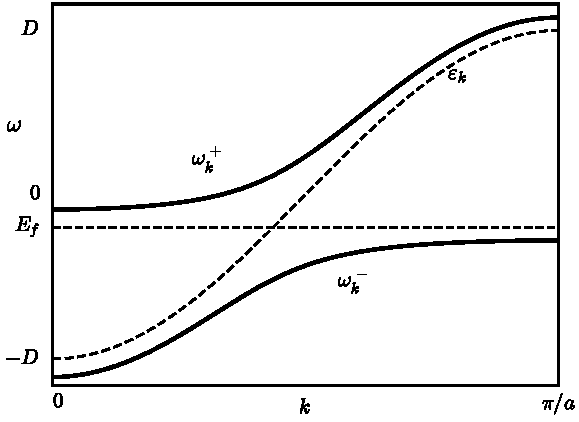
\includegraphics[width=7.5cm]{fig11-15.pdf}\\{\small 图 11.15\quad 重整杂化带的示意图，其中设\\
$\varepsilon_{k}=D\cos(ka)$，$E_{\mathrm{f}}=-0.2D$，$\widetilde{V}^{2}=0.1D$}
\end{minipage}
\end{center}

利用 $B=(\omega-\omega_{k}^{+})(\omega-\omega_{k}^{-})$ 以及 $(\omega-E_{\mathrm{f}})=-(\partial B/\partial\varepsilon_{k})$ 和 $(\omega-\varepsilon_{k})=-(\partial B/\partial E_{\mathrm{f}})$，类似于从式(11.1.50)导出式(11.1.51)的做法，可将c与f电子在k空间的格林函数写成下列标准形式
\begin{equation}
\begin{aligned}
  \langle\langle C_{km}|C_{km}^{+}\rangle\rangle_{\omega}
  &=\frac{A_{k}^{+}}{\omega-\omega_{k}^{-}}+\frac{A_{k}^{-}}{\omega-\omega_{k}^{+}}\\
  \langle\langle f_{km}|f_{km}^{+}\rangle\rangle_{\omega}
  &=\frac{A_{k}^{-}}{\omega-\omega_{k}^{-}}+\frac{A_{k}^{+}}{\omega-\omega_{k}^{+}}
\end{aligned}
\end{equation}
其中
\begin{equation}
  A_{k}^{\pm}=\frac{1}{2}\biggl\{1\pm\frac{(\varepsilon_{k}-E_{\mathrm{f}})}
  {\sqrt{(\varepsilon_{k}-E_{\mathrm{f}})^{2}+4\widetilde{V}^{2}}}\biggr\}
\end{equation}
并有 $A_{k}^{+}+A_{k}^{-}=1$ 关系.

为了便于计算重费密子系统中c电子与f电子的局域态密度(简称c-DOS与f-DOS)，我们将引入下列平均的格点格林函数：
\begin{subequations}
\begin{equation}
  G_{\mathrm{c}}(\omega)\equiv\frac{1}{N}\sum_{l}\langle\langle C_{lm}|C_{lm}^{+}\rangle\rangle_{\omega}
  =\frac{1}{N}\sum_{k}\langle\langle C_{km}|C_{km}^{+}\rangle\rangle_{\omega}
\end{equation}
\begin{equation}
  G_{\mathrm{f}}(\omega)\equiv\frac{1}{N}\sum_{l}\langle\langle f_{lm}|f_{lm}^{+}\rangle\rangle_{\omega}
  =\frac{1}{N}\sum_{k}\langle\langle f_{km}|f_{km}^{+}\rangle\rangle_{\omega}
\end{equation}
\begin{equation}
  G_{\mathrm{cf}}(\omega)\equiv G_{\mathrm{fc}}(\omega)
  =\frac{1}{N}\sum_{k}\langle\langle C_{km}|f_{km}^{+}\rangle\rangle_{\omega}
\end{equation}
\end{subequations}
根据式(11.1.39)，c-DOS 与 f-DOS 可简单地表示为
\begin{subequations}
\begin{equation}
  \rho_{\mathrm{c}}(\omega)=-\frac{1}{\pi}\mathrm{Im}\,G_{\mathrm{c}}(\omega+\mathrm{i}\eta)
\end{equation}
\begin{equation}
  \rho_{\mathrm{f}}(\omega)=-\frac{1}{\pi}\mathrm{Im}\,G_{\mathrm{f}}(\omega+\mathrm{i}\eta)
\end{equation}
\end{subequations}
其中 $\eta=0^{+}$，再利用格林函数解式(11.8.2)，又可将格点的推迟格写成
\begin{subequations}
\begin{equation}
  G_{\mathrm{c}}(\omega+\mathrm{i}\eta)=\frac{1}{N}\sum_{k}
  \biggl[(\omega-\varepsilon_{k})-\frac{\widetilde{V}^{2}}{(\omega-E_{\mathrm{f}})}+\mathrm{i}\eta\biggr]^{-1}
\end{equation}
\begin{equation}
  G_{\mathrm{f}}(\omega+\mathrm{i}\eta)=\frac{\widetilde{V}^{2}}{(\omega-E_{\mathrm{f}}+\mathrm{i}\eta)^{2}}
  G_{\mathrm{c}}(\omega+\mathrm{i}\eta)+\frac{1}{(\omega-E_{\mathrm{f}}+\mathrm{i}\eta)}
\end{equation}
\begin{equation}
  G_{\mathrm{cf}}(\omega+\mathrm{i}\eta)=\frac{\widetilde{V}}{(\omega-E_{\mathrm{f}})}
  G_{\mathrm{c}}(\omega+\mathrm{i}\eta)
\end{equation}
\end{subequations}
将应用于推导 c-DOS 与 f-DOS 的表示式.

\subsection*{2. 局域态密度}

我们将首先介绍重费密子系统中的c-DOS、f-DOS 以及准粒子态密度与未微扰的导带态密度 $\rho_{\mathrm{c}}^{(0)}(\omega)$ 之间的普遍关系式，然后再采用简化的矩形未微扰导带态密度，给出文献中常见的c-DOS 与f-DOS 公式.

在 $G_{\mathrm{c}}(\omega+\mathrm{i}\eta)$ 的表示式(11.8.9a)中取 $\widetilde{V}=0$，再代入 c-DOS 公式(11.8.8)，可求出未微扰的导带电子态密度
\begin{equation}
  \rho_{\mathrm{c}}^{(0)}(\omega)=-\frac{1}{\pi N}\mathrm{Im}\sum_{k}(\omega-\varepsilon_{k}+\mathrm{i}\eta)^{-1}
  =\frac{1}{N}\sum_{k}\delta(\omega-\varepsilon_{k})
\end{equation}
这是独立粒子系统态密度的标准公式，$\rho_{\mathrm{c}}^{(0)}(\omega)$ 的具体表示式由能带 $\varepsilon_{k}$ 决定.计入重整杂化 $(\widetilde{V}=rV)$ 以后的 c-DOS 可将式(11.8.9a)代入式(11.8.8)，得到
\begin{subequations}
\begin{equation}
  \rho_{\mathrm{c}}(\omega)=-\frac{1}{\pi N}\mathrm{Im}\sum_{k}
  \biggl[\biggl(\omega-\frac{\widetilde{V}^{2}}{\omega-E_{\mathrm{f}}}\biggr)-\varepsilon_{k}+\mathrm{i}\eta\biggr]^{-1}
\end{equation}
并与 $\rho_{\mathrm{c}}^{(0)}(\omega)$ 的表示式相比较，求出一般关系式
\begin{equation}
  \rho_{\mathrm{c}}(\omega)=\rho_{\mathrm{c}}^{(0)}\biggl(\omega-\frac{\widetilde{V}^{2}}{\omega-E_{\mathrm{f}}}\biggr)
\end{equation}
\end{subequations}
类似地，计入重整杂化 $\widetilde{V}$ 以后的f-DOS 可根据式(11.8.9b)写为
\begin{subequations}
\begin{equation}
  \rho_{\mathrm{f}}(\omega)=-\frac{1}{\pi}\mathrm{Im}\biggl[
  \frac{\widetilde{V}^{2}}{(\omega-E_{\mathrm{f}}+\mathrm{i}\eta)^{2}}G_{\mathrm{c}}(\omega+\mathrm{i}\eta)
  +\frac{1}{(\omega-E_{\mathrm{f}}+\mathrm{i}\eta)}\biggr]
\end{equation}
经直接复数运算后，可将等式右边写为
\begin{equation*}
\begin{aligned}
  \frac{\widetilde{V}^{2}}{(\omega-E_{\mathrm{f}})^{2}}\biggl[-\frac{1}{\pi}\mathrm{Im}\,G_{\mathrm{c}}(\omega+\mathrm{i}\eta)\biggr]
  &+\frac{1}{N}\sum_{k}\frac{(\omega-\varepsilon_{k})}{[(\omega-\varepsilon_{k})(\omega-E_{\mathrm{f}})-\widetilde{V}^{2}]}\\
  &\times(\omega-E_{\mathrm{f}})\delta(\omega-E_{\mathrm{f}})
\end{aligned}
\end{equation*}
其中的第二项，由于含 $(\omega-E_{\mathrm{f}})\delta(\omega-E_{\mathrm{f}})$ 因子，对求和无贡献.在物理上，这是由于 $(\omega-E_{\mathrm{f}}+\mathrm{i}\eta)^{-1}$ 及 $(\omega-E_{\mathrm{f}}+\mathrm{i}\eta)^{-2}$ 的极点 $\omega=E_{\mathrm{f}}$ 均不在重整杂化带之中(参考图11.15)，其虚部可以略去.因此 f-DOS 的一般表示式为
\begin{equation}
  \rho_{\mathrm{f}}(\omega)=\frac{\widetilde{V}^{2}}{(\omega-E_{\mathrm{f}})^{2}}\rho_{\mathrm{c}}(\omega)
  =\frac{\widetilde{V}^{2}}{(\omega-E_{\mathrm{f}})^{2}}\rho_{\mathrm{c}}^{(0)}
  \biggl(\omega-\frac{\widetilde{V}^{2}}{\omega-E_{\mathrm{f}}}\biggr)
\end{equation}
\end{subequations}
为了简化运算起见，在文献中常取矩形的未微扰导带态密度
\begin{equation}
  \rho_{\mathrm{c}}^{(0)}(\varepsilon)=\frac{1}{2D}\theta(\varepsilon+D)\theta(\varepsilon-D)
  =\begin{cases}
    \dfrac{1}{2D} & (-D<\varepsilon<+D)\\[2mm]
    0 & (|\varepsilon|>D)
  \end{cases}
\end{equation}
其中 $\theta$ 为阶跃函数，导带宽度为2D，$\varepsilon$ 的原点取在未微扰导带的中央.这一简化的矩形态密度相当于将费密面附近朗道费密液体的线性关系 $(\varepsilon_{k}\sim k)$ 拓宽到全导带 $(-D<\varepsilon<+D)$ 范围.这时重整杂化带中的 c-DOS 由
\begin{equation}
  \rho_{\mathrm{c}}(\omega)=\rho_{\mathrm{c}}^{(0)}[\varepsilon(\omega)]
\end{equation}
决定，其中
\begin{equation}
  \varepsilon(\omega)=\omega-\frac{\widetilde{V}^{2}}{(\omega-E_{\mathrm{f}})}
\end{equation}
而 $\varepsilon(\omega)$ 的带边在 $\varepsilon(\omega)=\pm D$ 处，也就是说带边由下列方程
\begin{equation}
  \omega^{2}-(E_{\mathrm{f}}\pm D)\omega-(\widetilde{V}^{2}\mp DE_{\mathrm{f}})=0
\end{equation}
的根决定.由此可求得重整杂化带的带边为
\begin{equation}
\left.\begin{aligned}
  \omega_{\mathrm{a}}&=\frac{1}{2}\bigl\{(E_{\mathrm{f}}-D)-\sqrt{(E_{\mathrm{f}}+D)^{2}+4\widetilde{V}^{2}}\bigr\}\\
  \omega_{\mathrm{b}}&=\frac{1}{2}\bigl\{(E_{\mathrm{f}}+D)-\sqrt{(E_{\mathrm{f}}-D)^{2}+4\widetilde{V}^{2}}\bigr\}\\
  \omega_{\mathrm{c}}&=\frac{1}{2}\bigl\{(E_{\mathrm{f}}-D)+\sqrt{(E_{\mathrm{f}}+D)^{2}+4\widetilde{V}^{2}}\bigr\}\\
  \omega_{\mathrm{d}}&=\frac{1}{2}\bigl\{(E_{\mathrm{f}}+D)+\sqrt{(E_{\mathrm{f}}-D)^{2}+4\widetilde{V}^{2}}\bigr\}
\end{aligned}\right\}
\end{equation}
其中重整杂化带的上、下带 $\omega_{k}^{\pm}$ 分别落在 $\omega_{\mathrm{a}}<\omega_{k}^{-}<\omega_{\mathrm{b}}$ 及 $\omega_{\mathrm{c}}<\omega_{k}^{+}<\omega_{\mathrm{d}}$ 区域中.因此 c-DOS 与f-DOS 均可利用阶跃函数表示为下列解析形式：
\begin{equation}
\left.\begin{aligned}
  \rho_{\mathrm{c}}(\omega)&=\frac{1}{2D}\bigl[\theta(\omega-\omega_{\mathrm{a}})\theta(\omega_{\mathrm{b}}-\omega)
  +\theta(\omega-\omega_{\mathrm{c}})\theta(\omega_{\mathrm{d}}-\omega)\bigr]\\
  \rho_{\mathrm{f}}(\omega)&=\biggl(\frac{1}{2D}\biggr)\frac{\widetilde{V}^{2}}{(\omega-E_{\mathrm{f}})^{2}}
  \bigl[\theta(\omega-\omega_{\mathrm{a}})\theta(\omega_{\mathrm{b}}-\omega)
  +\theta(\omega-\omega_{\mathrm{c}})\theta(\omega_{\mathrm{d}}-\omega)\bigr]
\end{aligned}\right\}
\end{equation}
或者更为明确地写成
\begin{equation}
  \rho_{\mathrm{c}}(\omega)=\begin{cases}
    \dfrac{1}{2D} & (\omega_{\mathrm{a}}<\omega<\omega_{\mathrm{b}}\ \text{及}\ \omega_{\mathrm{c}}<\omega<\omega_{\mathrm{d}}\ \text{或}\ \omega\in\omega_{k}^{\pm})\\[2mm]
    0 & (\text{在杂化带外})
  \end{cases}
\end{equation}
\begin{equation}
  \rho_{\mathrm{f}}(\omega)=\begin{cases}
    \dfrac{1}{2D}\dfrac{\widetilde{V}^{2}}{(\omega-E_{\mathrm{f}})^{2}} & (\omega\in\omega_{k}^{\pm})\\[2.5mm]
    0 & (\text{在杂化带外})
  \end{cases}
\end{equation}
图 11.16 是 $\rho_{\mathrm{c}}(\omega)$ 与 $\rho_{\mathrm{f}}(\omega)$ 的示意图，其中 $\rho_{\mathrm{c}}(\omega)$ 在重整杂化带内仍为常数，但 $\rho_{\mathrm{f}}(\omega)$ 则随 $(\omega-E_{\mathrm{f}})$ 的减小而增大，在靠近能隙处 f-DOS 远远高于c-DOS.当平均每格点的总电子数 $n_{\mathrm{t}}=n_{\mathrm{c}}+n_{\mathrm{f}}<\nu_{\mathrm{f}}$ 时，下带未被填满，化学势$\mu$在下带 $\omega_{k}^{-}$ 之内，系统属于重费密子金属.当 $\mu\in\omega_{k}^{-}$、$n_{\mathrm{t}}=\nu_{\mathrm{f}}$ 时，$n_{\mathrm{t}}N$ 个电子填满下带 $\omega_{k}^{-}$，它与全空的上带 $\omega_{k}^{+}$ 之间还隔着一个杂化所产生的非直接能隙，对应于重费密子半导体或近藤绝缘体.

\begin{center}
\begin{minipage}{6cm}
\centering
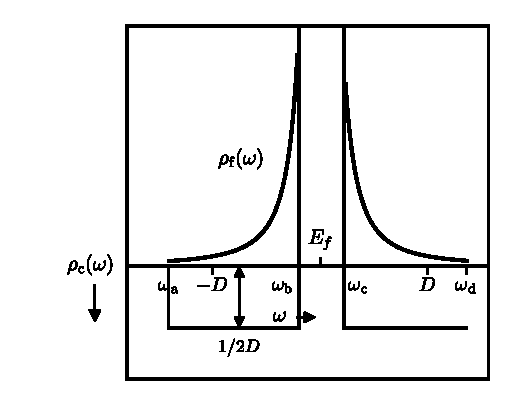
\includegraphics[width=6cm]{fig11-16.pdf}\\{\small 图 11.16\quad f-DOS 和 c-DOS 示意图}
\end{minipage}
\end{center}

重整杂化带的准粒子态密度 $\rho_{\mathrm{QP}}(\omega)$ 与 $\rho_{\mathrm{c}}(\omega)$、$\rho_{\mathrm{f}}(\omega)$ 之间有简单关系.由于 $H_{\mathrm{MF}}$ 可以严格对角化，从格林函数的极点所定出的 $\omega_{k}^{\pm}$ 就是重整杂化能带中的准粒子能量.在平均场近似下，准粒子间无相互作用，它们构成独立电子系统，根据独立粒子系统态密度的基本公式(2.8.7)，任一通道 m的准粒子态密度为
\begin{equation}
  \rho_{\mathrm{QP}}(\omega)=(1/N)\sum_{k}\delta(\omega-\omega_{k}^{-})+(1/N)\sum_{k}\delta(\omega-\omega_{k}^{+})
\end{equation}
另一方面，从c电子与f电子的格林函数表示式(11.8.5)，又可将 c-DOS 与 f-DOS 写成下列形式
\begin{subequations}
\begin{equation}
\begin{aligned}
  \rho_{\mathrm{c}}(\omega)&=-\Bigl(\frac{1}{\pi N}\Bigr)\mathrm{Im}\sum_{k}\biggl\{\frac{A_{k}^{+}}{\omega-\omega_{k}^{-}+\mathrm{i}\eta}
  +\frac{A_{k}^{-}}{\omega-\omega_{k}^{+}+\mathrm{i}\eta}\biggr\}\\
  &=(1/N)\sum_{k}\bigl\{A_{k}^{+}\delta(\omega-\omega_{k}^{-})+A_{k}^{-}\delta(\omega-\omega_{k}^{+})\bigr\}
\end{aligned}
\end{equation}
\begin{equation}
\begin{aligned}
  \rho_{\mathrm{f}}(\omega)&=-\Bigl(\frac{1}{\pi N}\Bigr)\mathrm{Im}\sum_{k}\biggl\{\frac{A_{k}^{-}}{\omega-\omega_{k}^{-}+\mathrm{i}\eta}
  +\frac{A_{k}^{+}}{\omega-\omega_{k}^{+}+\mathrm{i}\eta}\biggr\}\\
  &=\biggl(\frac{1}{N}\biggr)\sum_{k}\bigl\{A_{k}^{-}\delta(\omega-\omega_{k}^{-})+A_{k}^{+}\delta(\omega-\omega_{k}^{+})\bigr\}
\end{aligned}
\end{equation}
\end{subequations}
两式相加，并利用
\begin{equation*}
  A_{k}^{+}+A_{k}^{-}=1
\end{equation*}
立刻得到准粒子态密度式(11.8.21).因此，有关系式
\begin{equation}
  \rho_{\mathrm{QP}}(\omega)=\rho_{\mathrm{c}}(\omega)+\rho_{\mathrm{f}}(\omega)
\end{equation}
说明c与f电子态密度之和即准粒子态密度，用于计算重费密子系统的热力学量.

\subsection*{3. 自洽方程的零温解}

现在讨论自洽方程组式(11.7.29a)与式(11.7.29b)的低温解，目的在于求出隶玻色子平均场参量 $r^{2}(=1-n_{\mathrm{f}})$ 和 $\lambda\ (=E_{\mathrm{f}}-E_{0})$ 的零温解，并讨论系统的属性，用于重费密子金属和近藤绝缘体.

利用格林函数的谱定理
\begin{equation*}
  \langle BA\rangle=\int_{-\infty}^{\infty}\mathrm{d}\omega f(\omega)
  \biggl[-\frac{1}{\pi}\mathrm{Im}\,\langle\langle A|B\rangle\rangle_{\omega+\mathrm{i}\eta}\biggr]
\end{equation*}
和平均的格点格林函数表示式(11.8.9)可将 $r^{2}$ 与λ的自洽方程分别改写为下列表示式.对于 $r^{2}$ 的自洽方程
\begin{equation}
\begin{aligned}
  1-r^{2}=n_{\mathrm{f}}&=\frac{1}{N}\sum_{k,m}\langle f_{km}^{+}f_{km}\rangle_{\mathrm{MF}}\\
  &=\frac{-1}{\pi}\sum_{m}\int_{-\infty}^{\infty}\mathrm{d}\omega f(\omega)\mathrm{Im}
  \biggl\{\frac{1}{N}\sum_{k}\langle\langle f_{km}|f_{km}^{+}\rangle\rangle_{\omega+\mathrm{i}\eta}\biggr\}\\
  &=\nu_{\mathrm{f}}\int_{-\infty}^{\infty}\mathrm{d}\omega f(\omega)
  \biggl\{\biggl(-\frac{1}{\pi}\biggr)\mathrm{Im}\,G_{\mathrm{f}}(\omega+\mathrm{i}\eta)\biggr\}\\
  &=\nu_{\mathrm{f}}\int_{-\infty}^{\infty}\mathrm{d}\omega f(\omega)\rho_{\mathrm{f}}(\omega)
\end{aligned}
\end{equation}
上式表明，任一格点上的平均f电子数 $n_{\mathrm{f}}$ 可直接从 f-DOS 计算.类似的，对于λ的自洽方程
\begin{equation}
\begin{aligned}
  -r\lambda=r(E_{0}-E_{\mathrm{f}})&=\frac{V}{N}\sum_{k,m}\langle f_{km}^{+}C_{km}\rangle_{\mathrm{MF}}\\
  &=\nu_{\mathrm{f}}V\int_{-\infty}^{\infty}\mathrm{d}\omega f(\omega)
  \biggl\{\biggl(-\frac{1}{\pi}\biggr)\mathrm{Im}\,G_{\mathrm{cf}}(\omega+\mathrm{i}\eta)\biggr\}\\
  &=\nu_{\mathrm{f}}V\int_{-\infty}^{\infty}\mathrm{d}\omega f(\omega)\frac{rV}{(\omega-E_{\mathrm{f}})}
  \biggl\{\biggl(-\frac{1}{\pi}\biggr)\mathrm{Im}\,G_{\mathrm{c}}(\omega+\mathrm{i}\eta)\biggr\}\\
  &=\nu_{\mathrm{f}}rV^{2}\int_{-\infty}^{\infty}\mathrm{d}\omega f(\omega)
  \frac{1}{(\omega-E_{\mathrm{f}})}\rho_{\mathrm{c}}(\omega)
\end{aligned}
\end{equation}
再将 $\rho_{\mathrm{c}}$ 与 $\rho_{\mathrm{f}}$ 的具体表示式(11.8.19)与(11.8.20)分别代入上述两式，即可求出 $r^{2}$ 与λ的解.

对于 $n_{\mathrm{t}}<\nu_{\mathrm{f}}$ 的金属情形，化学势 $\boldsymbol{\mu}$ 位于下带 $\omega_{k}^{-}$ 之中，这时 $n_{\mathrm{f}}$ 与 $E_{\mathrm{f}}$（或 $r^{2}$ 与λ)的零温解可以直接求出为
\begin{equation}
  n_{\mathrm{f}}=\frac{\nu_{\mathrm{f}}}{2D}\int_{\omega_{\mathrm{a}}}^{\mu}
  \frac{r^{2}V^{2}}{(\omega-E_{\mathrm{f}})^{2}}\mathrm{d}\omega
  =\frac{\nu_{\mathrm{f}}r^{2}V^{2}}{2D}\biggl\{\frac{1}{(E_{\mathrm{f}}-\mu)}-\frac{1}{(E_{\mathrm{f}}-\omega_{\mathrm{a}})}\biggr\}
\end{equation}
\begin{equation}
  E_{0}-E_{\mathrm{f}}=\frac{\nu_{\mathrm{f}}V^{2}}{2D}\int_{\omega_{\mathrm{a}}}^{\mu}
  \frac{\mathrm{d}\omega}{(\omega-E_{\mathrm{f}})}
  =\frac{\nu_{\mathrm{f}}V^{2}}{2D}\ln\biggl[\frac{(E_{\mathrm{f}}-\mu)}{(E_{\mathrm{f}}-\omega_{\mathrm{a}})}\biggr]
\end{equation}
其中化学势$\mu$由总粒子数 $n_{\mathrm{t}}$ 的守恒条件式(11.7.30)决定，其零温表示式为
\begin{equation}
  n_{\mathrm{t}}=n_{\mathrm{f}}+\nu_{\mathrm{f}}(\mu-\omega_{\mathrm{a}})/2D
\end{equation}
由于强关联将导致f电子局域化，因此在 $U\to\infty$ 时的重整杂化 $\widetilde{V}\ (\widetilde{V}=rV)$ 将比原来的杂化V小得多，再考虑到通常 $V/D<1$，我们有理由认为未微扰的导带半宽度 $D\gg\widetilde{V}$，这时带边值公式(11.8.17)可近似为
\begin{equation}
\left.\begin{aligned}
  \omega_{\mathrm{a}}&\approx-D-r^{2}V^{2}/(D+E_{\mathrm{f}})\\
  \omega_{\mathrm{b}}&\approx E_{\mathrm{f}}-r^{2}V^{2}/(D-E_{\mathrm{f}})\\
  \omega_{\mathrm{c}}&\approx E_{\mathrm{f}}+r^{2}V^{2}/(D+E_{\mathrm{f}})\\
  \omega_{\mathrm{d}}&\approx D+r^{2}V^{2}/(D-E_{\mathrm{f}})
\end{aligned}\right\}
\end{equation}
考虑到 $\omega_{\mathrm{a}}\approx-D$，式(11.8.26)右边的第二项为 $D^{-2}$ 量级可以略去，求得
\begin{equation}
  n_{\mathrm{f}}=1-r^{2}\approx\frac{\nu_{\mathrm{f}}r^{2}V^{2}}{2D(E_{\mathrm{f}}-\mu)}
\end{equation}
上式又可改写为
\begin{equation}
  \frac{E_{\mathrm{f}}-\mu}{D}\approx\biggl(\frac{\nu_{\mathrm{f}}}{2}\biggr)\biggl(\frac{V}{D}\biggr)^{2}\frac{r^{2}}{1-r^{2}}
\end{equation}
显然，$(E_{\mathrm{f}}-\mu)/D$ 是量级为 $r^{2}$ 的小量，在重费密子系统中可以根据 $D\gg\widetilde{V}$ 与 $(E_{\mathrm{f}}-\mu)$ 作近似求出 $n_{\mathrm{f}}$、$E_{\mathrm{f}}$ 及 $\boldsymbol{\mu}$ 的近似表示式.为此，引入下列符号定义
\begin{equation}
  k_{\mathrm{B}}T_{\mathrm{L}}\equiv E_{\mathrm{f}}-\mu,\quad
  \Gamma\equiv\pi V^{2}/2D,\quad
  \widetilde{\Gamma}\equiv\pi r^{2}V^{2}/2D
\end{equation}
其中 $\Gamma$ 代表不计杂化V的重整效应(即取 $r=1$)时安德逊模型中f能级的共振线宽度，与式(11.6.21)中的 $\Gamma$ 是类似的.$T_{\mathrm{L}}$ 是安德逊晶格模型的一个特征温度，$k_{\mathrm{B}}T_{\mathrm{L}}$ 就是从费密面算起的重整f能级.按此，可写出式(11.8.26)—(11.8.28)等3个基本方程的近似表示式
\begin{subequations}
\begin{equation}
  n_{\mathrm{f}}=\nu_{\mathrm{f}}\widetilde{\Gamma}/\pi k_{\mathrm{B}}T_{\mathrm{L}}
  =1-(\widetilde{\Gamma}/\Gamma)=1-r^{2}
\end{equation}
\begin{equation}
  (E_{0}-\mu)-k_{\mathrm{B}}T_{\mathrm{L}}=(\nu_{\mathrm{f}}\Gamma/\pi)\ln[k_{\mathrm{B}}T_{\mathrm{L}}/(D+\mu)]
\end{equation}
\begin{equation}
  n_{\mathrm{t}}=n_{\mathrm{f}}+\nu_{\mathrm{f}}(\mu+D)/2D
\end{equation}
\end{subequations}
从式(11.8.33a)立刻求得 $T=0$ K时
\begin{equation}
  n_{\mathrm{f}}=\frac{1}{1+\pi k_{\mathrm{B}}T_{\mathrm{L}}/\nu_{\mathrm{f}}\Gamma}
\end{equation}
当未微扰的f能级远低于费密能级时，即 $E_{0}-\mu\ll 0$ 并取很大的负值时，可略去式(11.8.33b)左边的 $k_{\mathrm{B}}T_{\mathrm{L}}$ 项，求得特征温度满足
\begin{equation}
  k_{\mathrm{B}}T_{\mathrm{L}}=(D+\mu)\exp\biggl(-\frac{\pi|E_{0}-\mu|}{\nu_{\mathrm{f}}\Gamma}\biggr)
\end{equation}
特别是在近藤极限下，当 $|E_{0}-\mu|\gg\Gamma$ 时，$k_{\mathrm{B}}T_{\mathrm{L}}$ 将比 $(D+\mu)$ 小几个数量级，可以认为式(11.8.34)中的 $(\pi k_{\mathrm{B}}T_{\mathrm{L}}/\nu_{\mathrm{f}}\Gamma)$ 也是一个小参量，展开后求得 $n_{\mathrm{f}}=1-r^{2}\approx 1-(\pi k_{\mathrm{B}}T_{\mathrm{L}}/\nu_{\mathrm{f}}\Gamma)$，其中 $r^{2}\approx(\pi k_{\mathrm{B}}T_{\mathrm{L}}/\nu_{\mathrm{f}}\Gamma)\ll 1$.这时每格点的平均f电子数 $n_{\mathrm{f}}$ 趋近1，但仍然保持为略小于1的近整数，安德逊晶格系统中仍然存在很弱的重整杂化 $\widetilde{V}=rV$（其中 $r^{2}\ll 1$）.因此，人们常将安德逊晶格的近藤极限称为近整数价极限.同时，仍然存在的弱f-c杂化 $\widetilde{V}$，将使f电子成为近局域化的弱巡游电子，导致重费密子特性.

重电子金属中的重费密子特性，在实验上表现为零温比热容系数 $\gamma(0)$ 比普通金属至少高两个量级，在理论上表现为低激发态具有很高的电子有效质量 $(m^{*}/m_{\mathrm{e}})\gg 1$.我们将指出，以上结果均来源于费密面上f电子的态密度 $\rho_{\mathrm{f}}(\mu)$ 远远高于传导电子的态密度 $\rho_{\mathrm{c}}(\mu)$.根据态密度公式(11.8.18)与(11.8.19)可知
\begin{equation}
  \frac{\rho_{\mathrm{f}}(\mu)}{\rho_{\mathrm{c}}(\mu)}=\frac{\widetilde{V}^{2}}{(E_{\mathrm{f}}-\mu)^{2}}
  \approx\biggl(\frac{2}{\nu_{\mathrm{f}}}\biggr)\frac{n_{\mathrm{f}}D}{k_{\mathrm{B}}T_{\mathrm{L}}}\gg 1
\end{equation}
在第二个等式中利用了式(11.8.30)和定义式(11.8.32).显然，在近藤极限可取 $n_{\mathrm{f}}\approx 1$，并设 $\nu_{\mathrm{f}}=2$，则上式右边简化为 $(D/k_{\mathrm{B}}T_{\mathrm{L}})$，因此 $\rho_{\mathrm{f}}(\mu)\gg\rho_{\mathrm{c}}(\mu)$.在固体物理学中已知金属中费密面上任一自旋取向的态密度
\begin{equation}
  \rho(\mu)=\frac{3n}{4E_{\mathrm{F}}}=\frac{m^{*}k_{\mathrm{F}}}{2\pi^{2}h^{2}}
\end{equation}
其中 $m^{*}$ 是电子的有效质量.若取传导电子的有效质量为自由电子质量 $m_{\mathrm{e}}$，并认为重的金属中的高有效质量主要来自f电子，则在近藤极限下取 $\nu_{\mathrm{f}}=2$ 可得
\begin{equation}
  \frac{m^{*}}{m_{\mathrm{e}}}=\frac{\rho_{\mathrm{f}}(\mu)}{\rho_{\mathrm{c}}(\mu)}
  \approx\frac{D}{k_{\mathrm{B}}T_{\mathrm{L}}}\gg 1
\end{equation}
显然，$(E_{\mathrm{f}}-\mu)\equiv k_{\mathrm{B}}T_{\mathrm{L}}$ 取小的正值将导致重费密子效应.从物理角度分析，由于强关联产生的f能级重整化，使f电子从远低于 $\mu$ 的 $E_{0}$ 提升到略高于 $\boldsymbol{\mu}$ 的 $E_{\mathrm{f}}\ (E_{\mathrm{f}}=E_{0}+\lambda)$ 处，并保持 $0<(E_{\mathrm{f}}-\mu)\ll D$，如图11.16所示.从图可知，由于 $E_{\mathrm{f}}$ 位于杂化能隙之中，化学势 $\mu$ 必然落在下带 $\omega_{k}^{-}$ 曲线的平坦变化部分，自然具有很高的准粒子有效质量.

零温时重电子金属的线性比热容系数可从费密面上的准粒子态密度 $\rho_{\mathrm{QP}}(\mu)$ 求出
\begin{equation}
\begin{aligned}
  \gamma(0)&=\nu_{\mathrm{f}}\frac{\pi^{2}k_{\mathrm{B}}^{2}}{3}\rho_{\mathrm{QP}}(\mu)
  =\nu_{\mathrm{f}}\frac{\pi^{2}k_{\mathrm{B}}^{2}}{3}\bigl[\rho_{\mathrm{c}}(\mu)+\rho_{\mathrm{f}}(\mu)\bigr]\\
  &=\nu_{\mathrm{f}}\frac{\pi^{2}k_{\mathrm{B}}^{2}}{3}\biggl[\frac{1}{2D}+\frac{r^{2}V^{2}}{2D(E_{\mathrm{f}}-\mu)^{2}}\biggr]\\
  &=\nu_{\mathrm{f}}\frac{\pi^{2}k_{\mathrm{B}}^{2}}{3}\biggl(\frac{1}{2D}+\frac{n_{f}}{\nu_{\mathrm{f}}k_{\mathrm{B}}T_{\mathrm{L}}}\biggr)
\end{aligned}
\end{equation}
其中利用了式(11.8.30).在普通金属中，由于不存在近局域的f电子，其零温线性比热容系数 $\gamma_{0}(0)$ 可由上式右边第一项表示
\begin{equation}
  \gamma_{0}(0)=\frac{\nu_{\mathrm{f}}\pi^{2}k_{\mathrm{B}}^{2}}{3}\rho_{\mathrm{c}}(\mu)
\end{equation}
当取 $\nu_{\mathrm{f}}=2$ 时，就得到固体物理学中零温比热容系数的标准公式.因此重电子金属与普通金属的零温比热容系数满足下列不等式关系：
\begin{equation}
  \gamma(0)/\gamma_{0}(0)=1+\biggl(\frac{2}{\nu_{\mathrm{f}}}\biggr)\frac{n_{\mathrm{f}}D}{k_{\mathrm{B}}T_{\mathrm{L}}}\gg 1
\end{equation}
与实验观测结果一致.

现在讨论系统的绝缘情形，当 $n_{\mathrm{t}}=\nu_{\mathrm{f}}$ 时准粒子谱的下带从 $\omega_{\mathrm{a}}$ 到 $\omega_{\mathrm{b}}$ 均被填满，上带则是全空的，中间隔着一个杂化能隙 $\Delta=\omega_{\mathrm{c}}-\omega_{\mathrm{b}}$，属于近藤绝缘体.这时可取 $\boldsymbol{\mu}=\boldsymbol{\omega}_{\mathrm{b}}$ 代入化学势方程式(11.8.28)，并利用定义 $(E_{\mathrm{f}}-\mu)\equiv k_{\mathrm{B}}T_{\mathrm{L}}$，可将近藤绝缘体的带边值近似写成下列相对于 $E_{\mathrm{f}}$ 的表示式：
\begin{equation}
\left.\begin{aligned}
  \omega_{\mathrm{a}}&=E_{\mathrm{f}}-2D(1-n_{\mathrm{f}}/\nu_{\mathrm{f}})-k_{\mathrm{B}}T_{\mathrm{L}}\\
  \omega_{\mathrm{b}}&=\mu=E_{\mathrm{f}}-k_{\mathrm{B}}T_{\mathrm{L}}\\
  \omega_{\mathrm{c}}&=E_{\mathrm{f}}+(2n_{\mathrm{f}}/\nu_{\mathrm{f}})k_{\mathrm{B}}T_{\mathrm{L}}\\
  \omega_{\mathrm{d}}&=E_{\mathrm{f}}+(2n_{\mathrm{f}}/\nu_{\mathrm{f}})D+(2n_{\mathrm{f}}/\nu_{\mathrm{f}})k_{\mathrm{B}}T_{\mathrm{L}}
\end{aligned}\right\}
\end{equation}
其中
\begin{equation}
  E_{\mathrm{f}}=D(1-2n_{\mathrm{f}}/\nu_{\mathrm{f}})+(1-2n_{\mathrm{f}}/\nu_{\mathrm{f}})k_{\mathrm{B}}T_{\mathrm{L}}
\end{equation}
在求解式(11.8.27)时，近似取 $E_{\mathrm{f}}-\omega_{\mathrm{a}}=2D(1-n_{\mathrm{f}}/\nu_{\mathrm{f}})$，可将近藤绝缘体的特征温度表示为
\begin{equation}
  k_{\mathrm{B}}T_{\mathrm{L}}=2D(1-n_{\mathrm{f}}/\nu_{\mathrm{f}})
  \exp\biggl(-\frac{\pi|E_{0}-\mu|}{\nu_{\mathrm{f}}\Gamma}\biggr)
\end{equation}
类似于金属情形，近藤绝缘体的特征温度在近藤极限(当 $|E_{0}-\mu|\gg\Gamma$ 时)也是很低的，并满足 $k_{\mathrm{B}}T_{\mathrm{L}}\ll D$ 条件.近藤绝缘体中的能隙 $\Delta$ 可以利用式(11.8.42)写成 $k_{\mathrm{B}}T_{\mathrm{L}}$ 的表示式
\begin{equation}
  \Delta=\omega_{\mathrm{c}}-\omega_{\mathrm{b}}=(1+2n_{\mathrm{f}}/\nu_{\mathrm{f}})k_{\mathrm{B}}T_{\mathrm{L}}
\end{equation}
显然，能隙正比于特征温度，很低的特征温度 $T_{\mathrm{L}}$，将使近藤绝缘体呈现小能隙半导体特征.在 $\mathrm{Ce_{3}Bi_{4}Pt_{3}}$ 等近藤绝缘体材料中，$\Delta$ 只有 meV量级，它很容易因加压、外场和掺杂而改变.此外，从式(11.8.31)还可以看出 $\Delta\approx 2r^{2}V^{2}/D^{2}$，其中 SB 平均场参量 $r^{2}$ 是温度的函数，通过在有限温度解自洽方程式(11.8.24)与(11.8.25)，可求出 $r^{2}(T)$ 随温度升高而减小.因此，近藤绝缘体中的能隙也是温度的函数 $\Delta=\Delta(T)$，并将随升温而消失，使近藤绝缘体过渡为重费密子金属，与实验观测一致.理论上，$\Delta=\Delta(T)$ 来源于多体效应，正是由于费密海中的传导电子与每个元胞中的f电子发生多体杂化效应，使能隙随温度变化，也使近藤绝缘体不同于通常的小能隙半导体，因为后者的能隙不随温度变化.

综上所述，在隶玻色子平均场理论中，存在一个很低的特征温度 $T_{\mathrm{L}}$ 是导致重费密子金属重费密子特性和近藤绝缘体的小能隙半导体特征的共同原因.

\section{t-J模型}

本节主要介绍在强关联极限下如何从单带赫伯德模型导出t-J模型.对适用于描述 $\mathrm{CuO_{2}}$ 平面低激发特征的推广t-J模型及其对铜氧化合物高温超导体的应用也将作定性的讨论.

\subsection*{1. t-J模型的导出}

将单带赫伯德模型写成下列形式
\begin{equation}
  H=-t\sum_{\langle ij\rangle,\sigma}(C_{i\sigma}^{+}C_{j\sigma}+h.c.)
  +U\sum_{i}n_{i\uparrow}n_{i\downarrow}
\end{equation}
相当于在紧束缚近似哈密顿量式(11.1.15)中令 $T_{0}=0$ 和 $|T_{1}|=t$，即取紧束缚近似能带的中央作为能量的原点，$\langle ij\rangle$ 代表最近邻的一对格点 $i$ 与 $j$，并约定对于每个对求和只进行一次，即 $C_{i\sigma}^{+}C_{j\sigma}$ 在约定求和号下仅描述从j向i格点的跃迁.至于从i至j的相反跃迁过程，则由厄米共轭项 $h.c.$ 表示.上式中的 t 又称近邻跃迁能量.当同格点的库仑排斥 $U=0$ 时，系统处于能带极限，所形成的紧束缚近似能带可容纳2N个电子，N为格点数.当每格点的平均电子数 $n=\langle n_{i\uparrow}\rangle+\langle n_{i\downarrow}\rangle=1$ 时，紧束缚近似能带为半满.正因如此，人们将计入库仑关联U项后的 $n=1$ 情形也称为赫伯德模型的半满情形.当 $t=0$ 而 $U\neq 0$ 时，系统处于原子极限.在前面的讨论中已严格证明：这时在任一格点上均有两个非简并的能级，其能级间距为U.当U与t都不为零，且 $(U/t)\gg 1$ 时称为赫伯德模型的强关联极限.在本章的§1“4”中已证明，由于电子在晶格中的跃迁将形成上、下两个子能带，每个子带中只能容纳N个电子，并且两子带中心相距大致为U.

现在讨论 $(U/t)\gg 1$ 和小于半满填充 $(n<1)$ 情形.根据近邻跃迁能量 $t=0$ 时在任一格点i上电子的可能占据情形，将格点i上的占据分为两类：其一是无双占格点态，包括空占据以及自旋朝上和朝下的单占据等3种；其二则是i格点的双占据态，描述同一格点被一对自旋取向相反电子占据的情形.推广到含有N个格点和 $N_{e}$ 个电子 $(N_{e}<N)$ 的晶格系统，设P为将系统投影到不含任何双占格点子空间中的投影算符，而 $Q=1-P$ 将代表另一投影算符，它将系统投影到含有双占格点的子空间.P算符的表示式十分简单
\begin{subequations}
\begin{equation}
  P=\prod_{i=1}^{N}(1-v_{i})\qquad(v_{i}\equiv n_{i\uparrow}n_{i\downarrow})
\end{equation}
显然在P子空间中不存在双占格点态，可简称为无双占子空间.在晶格系统中，Q算符的表示式比较复杂，它可以从下列连乘积的展开求得.设
\begin{equation}
\begin{aligned}
  \prod_{i}(x)&=\prod_{i=1}^{N}\bigl[(1-v_{i})+xv_{i}\bigr]\qquad(0\leqslant x\leqslant 1)\\
  &=P+\sum_{l=1}^{N}x^{l}Q_{l}
\end{aligned}
\end{equation}
其中
\begin{equation}
  Q_{l}=\sum_{(i_{1}\cdots i_{l})}\bigl[v_{i_{1}}\cdots v_{i_{l}}\prod'_{j}(1-v_{j})\bigr]
\end{equation}
代表系统中有l个格点为双占据，$\prod'_{j}$ 则是对 $(i_{1}\cdots i_{l})$ 以外的 $(N-l)$ 个格点的连乘.考虑到 $x=1$ 时的简单关系式 $\prod(1)=1$，可求出满足完备性条件 $P+Q=1$ 的Q表示式
\begin{equation}
  Q=\sum_{l=1}^{N}Q_{l}
\end{equation}
它包括了晶格系统中的所有可能双占情形.投影算符P与Q满足标准运算规律
\begin{equation}
  P^{2}=P,\ Q^{2}=Q,\ PQ=QP=0,\ P+Q=1
\end{equation}
其中还利用了费密子的算符等式
\begin{equation}
  n_{i\sigma}(1-n_{i\sigma})=0\quad\text{或}\quad v_{i}(1-v_{i})=0
\end{equation}
\end{subequations}
在对单带赫伯德模型作正则变换之前，定义
\begin{equation}
  H\equiv T+V,\ T\equiv-t\sum_{\langle ij\rangle,\sigma}(C_{i\sigma}^{+}C_{j\sigma}+h.c.),\
  V\equiv U\sum_{i}n_{i\uparrow}n_{i\downarrow}
\end{equation}
其中 $n_{i\sigma}=C_{i\sigma}^{+}C_{i\sigma}$，利用一个常规恒等式 $C_{i\sigma}=C_{i\sigma}[(1-n_{i\sigma})+n_{i\sigma}]$ 将H中的独立电子运动项 $T$ 直接划分为
\begin{equation}
\begin{aligned}
  T&=-t\sum_{\langle ij\rangle,\sigma}
  \bigl[(1-n_{i\overline{\sigma}})+n_{i\overline{\sigma}}\bigr]C_{i\sigma}^{+}C_{j\sigma}
  \bigl[(1-n_{j\overline{\sigma}})+n_{j\overline{\sigma}}\bigr]\\
  &=T_{\mathrm{h}}+T_{\mathrm{d}}+T_{\mathrm{mix}}
\end{aligned}
\end{equation}
其中
\begin{subequations}
\begin{equation}
  T_{\mathrm{h}}=-t\sum_{\langle ij\rangle,\sigma}(1-n_{i\overline{\sigma}})
  C_{i\sigma}^{+}C_{j\sigma}(1-n_{j\overline{\sigma}})+h.c.
\end{equation}
\begin{equation}
  T_{\mathrm{d}}=-t\sum_{\langle ij\rangle,\sigma}
  n_{i\overline{\sigma}}C_{i\sigma}^{+}C_{j\sigma}n_{j\overline{\sigma}}+h.c.
\end{equation}
\begin{equation}
  T_{\mathrm{mix}}=-t\sum_{\langle ij\rangle,\sigma}\bigl\{(1-n_{i\overline{\sigma}})
  C_{i\sigma}^{+}C_{j\sigma}n_{j\overline{\sigma}}
  +n_{i\overline{\sigma}}C_{i\sigma}^{+}C_{j\sigma}(1-n_{j\overline{\sigma}})+h.c.\bigr\}
\end{equation}
显然，$T_{\mathrm{h}}$代表电子从单占格点j向空占格点i的跃迁，跃迁发生在“下带”之中，描述“下带”中电子通过空占格点的运动项，简称“下带”空穴运动项.$T_{\mathrm{d}}$则是电子从双占格点j向单占格点i的跃迁，它将原来位于“上带”中 $j$ 格点上的第二个电子转移到i格点上，描述“上带”中的双占格点转移.利用式(11.9.2e)—(11.9.2f)易证 $PT_{\mathrm{d}}P=PT_{\mathrm{d}}Q=QT_{\mathrm{d}}P=0$ 和 $T_{\mathrm{d}}=QT_{\mathrm{d}}Q$，表明 $T_{\mathrm{d}}$ 仅出现在含有双占格点的Q子空间中.类似的 $V=U\sum_{i}n_{i\uparrow}n_{i\downarrow}$ 项也是仅仅出现在Q子空间中的项，并有 $V=QVQ$，其它项 $PVP=PVQ=QVP=0$.此外，$T_{\mathrm{mix}}$ 使“上带”与“下带”混合，属于带间跃迁项，正是它联系了“上带”与“下带”的运动.特别是在 $(U/t)\gg 1$ 和 $n<1$ 时，强关联将使“上带”不可能被电子实际占据，但是“上带”作为中间态仍可通过虚激发过程传递强关联效应对“下带”中电子运动的影响.因此 $T_{\mathrm{mix}}$ 项在推导t-J模型时是至关重要的.类似上文的讨论，易证 $PT_{\mathrm{mix}}P=QT_{\mathrm{mix}}Q=0$，再利用 $P+Q=1$ 求出
\begin{equation}
  T_{\mathrm{mix}}=PT_{\mathrm{mix}}Q+QT_{\mathrm{mix}}P=PTQ+QTP
\end{equation}
其中
\begin{equation}
  PT_{\mathrm{mix}}Q=-t\sum_{\langle ij\rangle,\sigma}(1-n_{i\overline{\sigma}})
  C_{i\sigma}^{+}C_{j\sigma}n_{j\overline{\sigma}}+h.c.=PTQ
\end{equation}
\begin{equation}
  QT_{\mathrm{mix}}P=-t\sum_{\langle ij\rangle,\sigma}
  n_{i\overline{\sigma}}C_{i\sigma}^{+}C_{j\sigma}(1-n_{j\overline{\sigma}})+h.c.=QTP
\end{equation}
\end{subequations}
以上结果进一步表明 $T_{\mathrm{mix}}$ 代表电子在两个子空间 P 与 Q之间的跃迁.

为了研究 $T_{\mathrm{mix}}$ 项的影响，再将赫伯德模型改写为
\begin{equation}
\left.\begin{aligned}
  H&=H_{0}+T_{\mathrm{mix}}\\
  H_{0}&=T_{\mathrm{h}}+T_{\mathrm{d}}+V
\end{aligned}\right\}
\end{equation}
注意，现在的 $H_{0}$ 中已包括了库仑关联项 V.利用正则变换式(5.5.8)—(5.5.11)，消去 $T_{\mathrm{mix}}$ 一阶项，求得准至二阶的有效哈密顿量
\begin{equation}
  H_{\mathrm{eff}}=\mathrm{e}^{-S}H\mathrm{e}^{S}=H_{0}+\frac{1}{2}[T_{\mathrm{mix}},S]
\end{equation}
其中变换的母函数 S 必须满足条件
\begin{equation}
  T_{\mathrm{mix}}+[H_{0},S]=0
\end{equation}
对应的矩阵元关系为
\begin{equation}
  (E_{m}-E_{n})\langle m|S|n\rangle=-\langle m|T_{\mathrm{mix}}|n\rangle
\end{equation}
$E_{m}$ 与 $E_{n}$ 分别是 $H_{0}$ 在 $|m\rangle$ 与 $|n\rangle$ 本征态的能量本征值.由此可将 S 写成
\begin{equation}
  S=\sum'_{m,n}|m\rangle\langle m|\frac{T_{\mathrm{mix}}}{(E_{n}-E_{m})}|n\rangle\langle n|
\end{equation}
其中 $|m\rangle\langle m|$ 与 $|n\rangle\langle n|$ 是投影算符的一般记号，它们分别可取 $P\,(Q)$ 与 $Q\ (P)$ 等两种能量本征值不相等的子空间算符，再利用式(11.9.5d)—(11.9.5f)，写出 S 的 P、Q 表示式
\begin{equation}
  S=\frac{PTQ-QTP}{E_{Q}-E_{P}}
\end{equation}
当 $U\gg t$ 时，$H_{0}$ 本征值在上、下子带间的能量差 $E_{Q}-E_{P}\approx U$，其中略去了含t的修正.因此，准至 $T_{\mathrm{mix}}$ 二阶的母函数
\begin{equation}
  S=\frac{PTQ-QTP}{U}
\end{equation}
或者更具体的表示为
\begin{equation}
  S=-(t/U)\sum_{\langle ij\rangle,\sigma}\bigl\{(1-n_{i\overline{\sigma}})C_{i\sigma}^{+}C_{j\sigma}n_{j\overline{\sigma}}
  -n_{i\overline{\sigma}}C_{i\sigma}^{+}C_{j\sigma}(1-n_{j\overline{\sigma}})+h.c.\bigr\}
\end{equation}
这时若将式(11.9.12)和(11.9.5d)代入 $H_{\mathrm{eff}}$ 的表示式(11.9.7)，经简单运算，求出
\begin{equation}
  H_{\mathrm{eff}}=T_{\mathrm{h}}+T_{\mathrm{d}}+V-\frac{1}{U}(PTQ)(QTP)+\frac{1}{U}(QTP)(PTQ)
\end{equation}
但上式仍然代表全希尔伯特空间中的有效哈密顿量，还必须排除双占据将系统限制在P子空间内，因为在强关联 $U\gg t$ 和不超过半满 $(n\leqslant 1)$ 情形，双占据格点实际上不可能出现，系统将被限制在无双占的P子空间中.这时才能求出单带赫伯德模型在强关联极限下描述系统低能激发的等效哈密顿量 $H_{\mathrm{eff}}^{P}$.为此作P投影，并利用 $PQ=QP=0$ 和 $PT_{\mathrm{d}}P=0$ 以及 $PVP=0$ 消去 Q 空间部分
\begin{equation}
  PH_{\mathrm{eff}}P=P\biggl\{T_{\mathrm{h}}-\frac{1}{U}(PTQ)(QTP)\biggr\}P\equiv PH_{\mathrm{eff}}^{P}P
\end{equation}
因此
\begin{equation}
  H_{\mathrm{eff}}^{P}=T_{\mathrm{h}}-\frac{1}{U}(PTQ)(QTP)
\end{equation}
在以后的讨论中略去 $H_{\mathrm{eff}}^{P}$ 的上、下标，简记为H.剩下的工作只是利用式(11.9.5)计算 $(PTQ)(QTP)/U$ 项.运算是直接的，但却较占篇幅，有兴趣的读者可参阅文献[29]，在那里求出了准至两格点求和项的P子空间有效哈密顿量
\begin{equation}
\left.\begin{aligned}
  &H=-t\sum_{\langle ij\rangle,\sigma}(\hat{C}_{i\sigma}^{+}\hat{C}_{j\sigma}+h.c.)
  +J\sum_{\langle i,j\rangle}\biggl(\hat{\boldsymbol{S}}_{i}\cdot\hat{\boldsymbol{S}}_{j}
  -\frac{1}{4}n_{i}n_{j}\biggr)\\
  &\hat{C}_{i\sigma}^{+}=(1-n_{i\overline{\sigma}})C_{i\sigma}^{+},\quad
   \hat{C}_{j\sigma}=C_{j\sigma}(1-n_{j\overline{\sigma}})\\
  &\hat{S}_{i}^{z}=\frac{1}{2}(C_{i\uparrow}^{+}C_{i\uparrow}-C_{i\downarrow}^{+}C_{i\downarrow}),\quad
   \hat{S}_{i}^{+}=C_{i\uparrow}^{+}C_{i\downarrow},\quad
   \hat{S}_{i}^{-}=C_{i\downarrow}^{+}C_{i\uparrow}
\end{aligned}\right\}
\end{equation}
其中 $\boldsymbol{n}_{i}$ 与 $\boldsymbol{n}_{j}$ 分别代表i与j格点的电子数密度算符，$J=(4t^{2}/U)>0$ 描述近邻自旋 $\hat{\boldsymbol{S}}_{i}$ 与 $\hat{\boldsymbol{S}}_{j}$ 之间的反铁磁交换作用.$\hat{C}_{i\sigma}^{+}=(1-n_{i\overline{\sigma}})C_{i\sigma}^{+}$ 与 $\hat{C}_{j\sigma}=C_{j\sigma}(1-n_{j\overline{\sigma}})$ 都是P子空间中的算符，其中要求 $j$ 为单占格点，而i格点应为空占据，H中等式右边第一项就是 $T_{\mathrm{h}}$，它描述电子通过空占格点的跃迁运动.此外，上式中的 $\hat{S}_{i}^{z}$ 与 $\hat{S}_{i}^{\pm}$ 就是人们熟知的自旋1/2算符的费密子表示式(11.6.10).在文献中常利用矢量泡利矩阵 $\hat{\boldsymbol{\sigma}}$，将它们概括为紧凑的矢量表示
\begin{equation}
  \hat{\boldsymbol{S}}_{i}=\frac{1}{2}\sum_{\alpha,\beta}C_{i\alpha}^{+}(\hat{\boldsymbol{\sigma}})_{\alpha\beta}C_{i\beta}
\end{equation}
其中 $\boldsymbol{\alpha}$ 与 $\beta$ 是自旋指标，它们均可取↑或↓，与前面的 $\sigma$ 标相同.式(11.9.7)中的 H 称为t-J模型.因此t-J模型就是单带赫伯德模型的强关联极限.自从高温超导体发现以来，t-J模型一直是研究 $\mathrm{CuO_{2}}$ 平面上二维强关联电子系统的一个重要理论模型.

由于 $T_{\mathrm{h}}$ 是被限制在P子空间中的空穴运动项，其跃迁项中往往涉及4个标准费密算子，将增加具体运算的困难.安德逊认为这一限制的物理机制主要是减小载流子的跃迁概率，可以作近似处理.引入平均每格点上的空穴浓度 $\delta\equiv 1-n$，它描述平均在每个格点上的空穴占据概率.对于 $\hat{C}_{i\sigma}^{+}=(1-n_{i\overline{\sigma}})C_{i\sigma}^{+}$ 可近似用 $\delta C_{i\sigma}^{+}$ 表示，而 $\hat{C}_{j\sigma}=C_{j\sigma}(1-n_{j\overline{\sigma}})$ 则近似用 $nC_{j\sigma}$ 代替，其中 $n=1-\delta$ 代表平均每个格点上电子占据的概率.这样，当系统接近半满$(n\to 1)$时，$\delta$ 很小，在准至 $\delta$ 一阶时可取 $(t\delta)$ 作为有效的跃迁能代替t，并将 $T_{\mathrm{h}}$ 近似用标准费密算子 $C_{i\sigma}^{+}$ 与 $C_{j\sigma}$ 的二次型表示.因此强关联与接近半满填充时t-J模型可写成
\begin{equation}
  H=-(t\delta)\sum_{\langle ij\rangle,\sigma}(C_{i\sigma}^{+}C_{j\sigma}+h.c.)
  +J\sum_{i,j}\biggl(\hat{\boldsymbol{S}}_{i}\cdot\hat{\boldsymbol{S}}_{j}-\frac{1}{4}n_{i}n_{j}\biggr)
\end{equation}
显然，未掺杂时 n = 1 和 $\delta=0$，没有荷电载流子的运动项，H中只剩 $J>0$ 海森伯交换作用项，这时系统的低能激发仅仅以反铁磁自旋波形式出现，即仅有自旋而无电荷自由度的激发.只有经过掺杂，当空穴被引入 $\mathrm{CuO_{2}}$ 平面后，荷电载流子才能在反铁磁背景中运动，这时系统中既有电荷又有自旋自由度，还包括这两种自由度之间的相互竞争.t-J模型以最简洁的形式概括了这一与高温超导体 $\mathrm{CuO_{2}}$ 平面特性密切相关的激发与竞争，使它成为凝聚态物理学中最受关注的模型之一.

\subsection*{2. t-J模型应用于母体化合物}

t-J模型是高温超导研究中的常用理论模型.铜氧化物高温超导体如 $(\mathrm{La}_{1-x}\mathrm{Sr}_{x})_{2}\mathrm{CuO_{4}}$ 系统，用 $\mathrm{Sr}^{2+}$ 离子作为杂质替代 $\mathrm{La}^{3+}$ 离子，将在 $\mathrm{CuO_{2}}$ 平面上引入空穴，当 $\boldsymbol{x}=\boldsymbol{0}$ 时系统是未掺杂的母体化合物La-214(即 $\mathrm{La}_{2}^{3+}\mathrm{Cu}^{2+}\mathrm{O}_{4}^{2-}$).由于 $\mathrm{Cu}^{2+}$ 的电子组态为 $(1\mathrm{s})^{2}\cdots(2\mathrm{p})^{6}\,(3\mathrm{d})^{9}$，其中d壳层是未填满的，因此在 $\mathrm{Cu}^{2+}$ 离子上只有一个自旋未配对的d电子，具有1/2自旋，处于 $3\mathrm{d}_{x^{2}-y^{2}}$ 态.在应用赫伯德模型讨论高温超导体特性时，人们往往不明显地考虑氧离子，而将 $\mathrm{CuO_{2}}$ 平面简单看成是铜离子的二维正方晶格，每个格点上的平均电子数 $n=1$，从理论上讲 $\mathrm{CuO_{2}}$ 平面属于单带赫伯德模型的半满情形.根据赫伯德模型的窄带强关联解，在Cu的二维正方晶格中，N个自旋为1/2的d电子仅填满“下带”，与全空的“上带”之间还被能隙隔开，系统的基态应当是绝缘体，但却不能进一步说明到底是顺磁的，铁磁的，还是反铁磁的绝缘体.铜氧化合物高温超导体的实验结果则进一步证实未掺杂的母体化合物如La-214等都是反铁磁的绝缘体.这一重要实验事实现在可以直接从t-J模型导出.由于此模型的 $H=T_{\mathrm{h}}+$（反铁磁背景项)，其中 $T_{\mathrm{h}}$ 只可能通过最近邻的空占格点跃迁.换句话说，在 $\mathrm{CuO_{2}}$ 平面上必须有空穴才可能出现 $T_{\mathrm{h}}$ 项.在 $U\gg t$ 和严格半满填充 $n=1$ 时，强关联$(U\gg t)$不允许双占格点出现，导致二维晶格中的 N个 d电子必然被N个格点所平分，而在每个格点上总是保持单占据，理论上可以用算符条件 $n_{i}=n_{j}=1$（其中 $n_{i}=n_{i\sigma}+n_{i\overline{\sigma}}$)表示这时 $\hat{C}_{i\sigma}^{+}=(1-n_{i\sigma})C_{i\sigma}^{+}$ 中的 $\sigma$ 自旋态根据泡利原理应为空占据，有 $n_{i\sigma}=0$，但是在取向相反的自旋态 $\overline{\sigma}$ 上，由于又应满足 $n_{i}=1$ 条件，则必须取 $n_{i\overline{\sigma}}=1$ 才能保持i格点在半满时的单占据特征.因此，$T_{\mathrm{h}}$ 中的一般跃迁项 $(1-n_{i\sigma})C_{i\sigma}^{+}C_{j\sigma}(1-n_{j\sigma})$ 在半满情况下必然消失，使 $T_{\mathrm{h}}=0$ 严格成立，其物理原因是由于半满时在 $\mathrm{CuO_{2}}$ 平面中无空穴，将使“下带”中电子无法运动.这样，在半满时t-J模型就直接简化为适用于绝缘磁体的反铁磁海森伯模型
\begin{equation}
  H=J\sum_{\langle ij\rangle}\hat{\boldsymbol{S}}_{i}\cdot\hat{\boldsymbol{S}}_{j}\qquad(J>0)
\end{equation}
其中仅略去了与自旋算符无关的C数项($-J/4$).这个绝缘系统的基态为取向朝上的自旋和取向朝下的自旋在二维正方晶格上交错的排列，朝上自旋的最近邻是朝下的自旋，形成反铁磁长程序，圆满地解释了超导母体化合物是反铁磁绝缘体的实验结果.以上讨论限于未掺杂的 $\boldsymbol{x}=\boldsymbol{0}$ 情形.

当掺杂浓度 $\boldsymbol{x}\neq\boldsymbol{0}$ 时，实验表明，随着x的增加反铁磁奈耳温度 $T_{\mathrm{N}}$ 将迅速下降.\allowbreak 在 $(\mathrm{La}_{1-x}\mathrm{Sr}_{x})_{2}\allowbreak\mathrm{CuO_{4}}$ 中大约 2\%的 Sr掺杂就完全破坏了反铁磁长程序，使 $T_{\mathrm{N}}$ 下降为零.另一方面，实验还证实了掺杂时空穴实际上是进入 $\mathrm{CuO_{2}}$ 平面的氧离子上，表明反铁磁长程序对于在氧离子上出现的空穴十分敏感.基于t-J模型，还可以定性地说明掺杂对于反铁磁序的破坏作用.掺杂后进入 $\mathrm{CuO_{2}}$ 平面中氧位的空穴使氧离子从 $\mathrm{O}^{2-}$ 变为 $\mathrm{O}^{-}$，而且氧空穴 $\mathrm{O}^{-}$ 的自旋与两边的 $\mathrm{Cu}^{2+}$ 自旋也有反铁磁交换作用，其交换作用强度还应当大于 $\mathrm{Cu}^{2+}-\mathrm{Cu}^{2+}$ 之间的反铁磁交换作用强度，因为氧位于两个最近邻铜离子之间，$\mathrm{Cu}^{2+}$ 与 $\mathrm{O}^{-}$ 的间距只是 $\mathrm{Cu}^{2+}-\mathrm{Cu}^{2+}$ 间距的一半.这将使氧空穴 $\mathrm{O}^{-}$ 两边的 $\mathrm{Cu}^{2+}$ 离子自旋取向从原来的反平行变为平行的排列，导致氧空穴周围的 $\mathrm{Cu}^{2+}$ 离子的反铁磁排列失配，从而破坏反铁磁长程序.

根据固体物理学，铜氧平面中的任一格点(或元胞)对应于一个 $\mathrm{CuO_{2}}$ 基元，每个元胞中含有一个Cu原子和两个O原子，共3个离子，构成二维复式晶格.未掺杂时，这些离子分别为 $\mathrm{Cu}^{2+}$ 和 $\mathrm{O}^{2-}$ 状态，其中两个氧离子的最高能级 $2\mathrm{p}_{x}$ 和 $2\mathrm{p}_{y}$ 轨道都已填满，只有 $\mathrm{Cu}^{2+}(3\mathrm{d}^{9}$ 组态)的 $3\mathrm{d}_{x^{2}-y^{2}}$ 轨道为半填满，仅含一个电子并具有自旋1/2.人们似乎可以不明显考虑氧，而把 $\mathrm{CuO_{2}}$ 平面简单看成是 $\mathrm{Cu}^{2+}$ 上电子自旋构成的反铁磁背景.但是，在进一步探索两个 $\mathrm{Cu}^{2+}$ 离子间反铁磁交换作用的成因时，$\mathrm{O}^{2-}$ 离子的中介作用是不可忽略的，下面我们将采用空穴描述对此作定性说明.

在高温超导研究中，人们习惯采用空穴描述，取满壳层的 $3\mathrm{d}^{10}(\mathrm{Cu}^{+})$ 与 $2\mathrm{p}^{6}(\mathrm{O}^{2-})$ 作为系统的真空，这时又可将未掺杂的 $\mathrm{CuO_{2}}$ 平面看成是在每一个格点的 $\mathrm{Cu}^{2+}$ 离子上有一个 $3\mathrm{d}_{x^{2}-y^{2}}$ 空穴并带有自旋，它们构成式(11.9.20)所描述的反铁磁背景，其中 $\hat{\boldsymbol{S}}_{i}$ 现在代表i格点上空穴的自旋算符.相应的在单带赫伯德模型中的 $C_{i\sigma}^{+}(C_{i\sigma})$ 也称作空穴的产生(消灭)算符，而U则是在铜离子上存在一对自旋取向相反的空穴间的库仑排斥.但应注意即使在未掺杂时，$\mathrm{CuO_{2}}$ 平面上的反铁磁交换作用J实际上来源于两个 $\mathrm{Cu}^{2+}$ 离子通过 $\mathrm{O}^{2-}$ 离子的超交换作用.物理上可以用三格点图像定性描述两个 $\mathrm{Cu}^{2+}$（用×表示)的自旋通过与 $\mathrm{O}^{2-}$ 离子（用○表示)之间的多次跃迁，并进行超交换的过程，如图11.17所示\textsuperscript{[30]}.设 $\varepsilon_{\mathrm{d}}$ 与 $\varepsilon_{\mathrm{p}}$ 分别代表Cu（×）与O(○)上空穴的能级，Cu-O 跃迁矩阵元为 $t_{\mathrm{pd}}\ (|t_{\mathrm{pd}}|\equiv t_{0})$，忽略氧上同时出现一对空穴时的库仑作用，只计及铜格点上的库仑关联U.在图11.17中，通道(a)的3个中间态与初态间能量差仅与铜氧间电荷转移能 $\Delta=\varepsilon_{\mathrm{p}}-\varepsilon_{\mathrm{d}}$ 有关.根据四阶微扰，两个 $\mathrm{Cu}^{2+}$ 空穴的自旋交换所降低的能量为 $2(t_{0}^{4}/\Delta^{3})$，出现因子2是由于在(a)通道还有一个等效的过程，其中左边的空穴自旋先向氧转移.类似的，(b)通道也包括两个等价的过程.在(b)中只有一个中间态是铜格点的空穴双占态，它与初态间能量差为U，其它两个中间态仍提供 $\Delta$ 能量差.因此，(b)通道因交换自旋所降低的能量为 $2(t_{0}^{4}/U\Delta^{2})$，这两个通道的贡献之和再乘以2才是在约定求和 $\langle ij\rangle$ 表示中的反铁磁超交换作用

\begin{center}
\begin{minipage}{7cm}
\centering
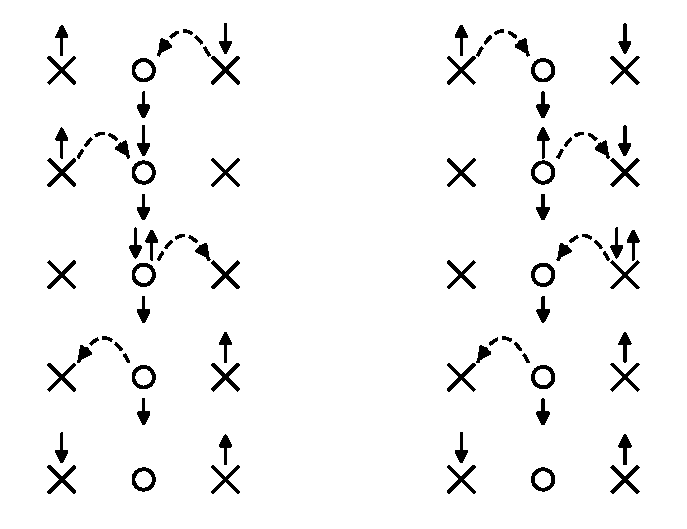
\includegraphics[width=7cm]{fig11-17.pdf}\\{\small (a) 不含U的通道\qquad (b) 含U的通道}\\[3pt]{\small 图 11.17\quad 铜空穴自旋间超交换的两个4阶通道：}
\end{minipage}
\end{center}

\begin{equation}
  J_{\mathrm{eff}}=\frac{4t_{0}^{4}}{\Delta^{2}}\biggl(\frac{1}{\Delta}+\frac{1}{U}\biggr)
  \approx\frac{4(t_{0}^{2}/\Delta)^{2}}{\Delta}
\end{equation}
在后一个等式中采用了近似条件 $U\gg\Delta$，略去(b)通道的贡献.高温超导的实验与理论研究已证明在 $\mathrm{CuO_{2}}$ 层中 $U>\Delta$，称为电荷转移情形，而未掺杂的母体化合物又称电荷转移型的反铁磁绝缘体.以上的定性讨论说明，对于未掺杂的 $\mathrm{CuO_{2}}$ 平面也必须考虑氧离子的作用，只有当超交换作用 $J_{\mathrm{eff}}$ 已求出并用它代替式(11.9.20)中的J以后，才能正确描述铜氧化合物.这时系统等效于半满单带赫伯德模型的强关联极限，其中仍然是 $\mathrm{Cu}^{2+}$ 空穴的自旋所构成的反铁磁背景，氧离子的作用已经包括在 $J_{\mathrm{eff}}$ 之中了.

\subsection*{3. 张-莱斯单态\textsuperscript{[31]}和推广的t-J模型}

在氧化物高温超导体发现的初期安德逊曾假定掺杂后进入 $\mathrm{CuO_{2}}$ 平面的多余空穴主要位于铜上并形成 $\mathrm{Cu}^{3+}$ 离子，物理上相当于多余空穴在 $\mathrm{Cu}^{2+}$ 离子构成的反铁磁背景中运动.正是基于这一假定，他首先提出采用单带赫伯德模型的强关联极限——t-J模型，描述高 $T_{\mathrm{c}}$ 铜氧化合物.但是，实验事实却与安德逊的假定相反，多余的空穴不是位于铜离子上，而是主要位于氧离子上，占据氧的 $2\mathrm{p}_{x}$ 或 $2\mathrm{p}_{y}$ 轨道，并与同一元胞内(或格点i上)的铜 $3\mathrm{d}_{x^{2}-y^{2}}$ 空穴轨道相耦合.单带赫伯德模型，由于未考虑氧离子的作用，已不再是合理的出发模型.人们必须构造一个明显含氧的 $2\mathrm{p}_{x}$、$2\mathrm{p}_{y}$ 和铜的 $3\mathrm{d}_{x^{2}-y^{2}}$ 空穴轨道在内的三带赫伯德模型，并用它描述 $\mathrm{CuO_{2}}$ 平面上的空穴运动才是正确的出发点.当存在多余空穴时，从三带赫伯德模型出发是否仍然可以用一个等效的单带t-J模型描述 $\mathrm{CuO_{2}}$ 平面的低激发特征？这个问题引起了大多数研究者的怀疑.张和莱斯\textsuperscript{[31]}在充分考虑了 Cu-O 杂化和 Cu 离子上强关联效应的情况下，首先证明了在 $\mathrm{CuO_{2}}$ 平面上的一个多余空穴，当它处于 $\mathrm{Cu}^{2+}$ 离子的4个近邻配位氧的对称组合轨道上时，将与此 $\mathrm{Cu}^{2+}$ 离子的 $3\mathrm{d}_{x^{2}-y^{2}}$ 轨道上的空穴之间通过杂化形成局域的单重态，将 $\mathrm{O}^{-}$ 空穴束缚在如图11.18所示的“方块”之中，这个 Cu-O 杂化的单重态被

\begin{center}
\begin{minipage}{6.5cm}
\centering
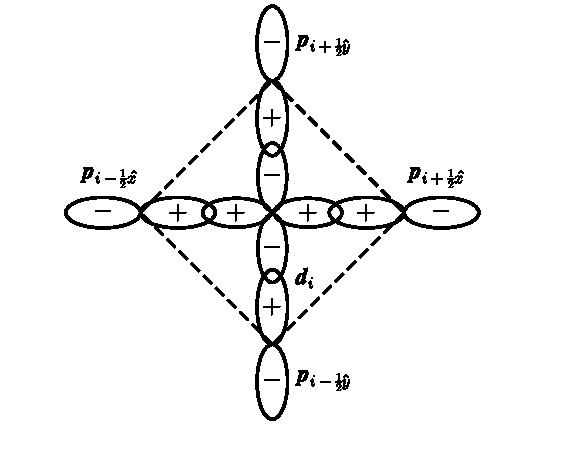
\includegraphics[width=6.5cm]{fig11-18.pdf}\\{\small 图 11.18\quad 氧空穴$(2\mathrm{p}^{5})$与铜空穴$(3\mathrm{d}^{9})$的杂化示意图.图中的“$\pm$”号代表波函数的相位}
\end{minipage}
\end{center}

称作张-莱斯单重态(ZRS).$\mathrm{CuO_{2}}$ 层的低激发态可以用 ZRS 在超交换反铁磁背景中的隧穿运动描述，等效于t-J模型，只是t现在应理解为ZRS在近邻格点间的跃迁能.张-莱斯的工作包括从三带简化为双带，再从双带系统演变为描述 $\mathrm{CuO_{2}}$ 平面低激发特征的等效单带系统.他们从三带模型出发
\begin{equation}
  H=\sum_{i,\sigma}\varepsilon_{\mathrm{d}}d_{i\sigma}^{+}d_{i\sigma}
  +\sum_{l,\sigma}\varepsilon_{\mathrm{p}}p_{l\sigma}^{+}p_{l\sigma}
  +U\sum_{i}n_{i\uparrow}^{d}n_{i\downarrow}^{d}+H'
\end{equation}
其中 $n_{i\sigma}^{d}=d_{i\sigma}^{+}d_{i\sigma}$，$d_{i\sigma}^{+}$ 是i 格点上 Cu 的 $3\mathrm{d}_{x^{2}-y^{2}}$ 空穴的产生算符，U是 Cu 格点的同位库仑排斥，$\varepsilon_{\mathrm{d}}$ 代表 Cu 的 $3\mathrm{d}_{x^{2}-y^{2}}$ 轨道能量.$p_{l\sigma}^{+}$ 表示在l位上O的 $2\mathrm{p}_{x}$ 和 $2\mathrm{p}_{y}$ 空穴的产生算符，可将它们分别写为 $l=i+\frac{1}{2}\hat{x}$ 和 $l=i+\frac{1}{2}\hat{y}$ 代表同一元胞内的两个氧位，$\varepsilon_{\mathrm{p}}$ 是 $2\mathrm{p}_{x}$ 与 $2\mathrm{p}_{y}$ 轨道能量.张和莱斯略去O的同位库仑排斥，O-O和 Cu-Cu 的直接跃迁项，仅考虑距离最近的 Cu-O 跃迁项，如图11.18所示，这时 H'可称作 Cu-O杂化项，并具体写为
\begin{equation}
  H'=t_{0}\sum_{i,\sigma}\biggl\{d_{i\sigma}^{+}\biggl(p_{i-\frac{1}{2}\hat{x},\sigma}
  +p_{i-\frac{1}{2}\hat{y},\sigma}-p_{i+\frac{1}{2}\hat{x},\sigma}
  -p_{i+\frac{1}{2}\hat{y},\sigma}\biggr)+h.c.\biggr\}
\end{equation}
其中 $t_{0}\,(=|t_{\mathrm{pd}}|)$ 代表 Cu-O跃迁矩阵元的数值，它正比于 Cu与O空穴波函数的重叠，此外还应考虑空穴波函数相位的影响.参考图11.18可知，对于 $i-\frac{1}{2}\hat{x}$ 与 $i-\frac{1}{2}\hat{y}$ 是相位一致情形，取$+$号，而 $i+\frac{1}{2}\hat{x}$ 与 $i+\frac{1}{2}\hat{y}$ 则代表相位相反的重叠应取$-$号.这里取 Cu-Cu间距为长度的单位，$\hat{\boldsymbol{x}}$ 与 $\hat{\boldsymbol{y}}$ 分别是x与$y$方向的单位矢量. Cu-O杂化项H'具有重要的对称特征.为了明显看出此特征，定义下列对称化的组合轨道态
\begin{equation}
  P_{i\sigma}=\frac{1}{2}\biggl(p_{i-\frac{1}{2}\hat{x}\sigma}+p_{i-\frac{1}{2}\hat{y}\sigma}
  -p_{i+\frac{1}{2}\hat{x}\sigma}-p_{i+\frac{1}{2}\hat{y}\sigma}\biggr)
\end{equation}
可将Cu-O杂化项，式(11.9.23)，更明确地表示为
\begin{equation}
  H'=2t_{0}\sum_{i,\sigma}(d_{i\sigma}^{+}P_{i\sigma}+h.c.)
\end{equation}
显然，Cu-O杂化仅仅发生在 $\mathrm{Cu}^{2+}$ 的 $3\mathrm{d}_{x^{2}-y^{2}}$ 轨道态与氧的对称组合轨道态 $P_{i\sigma}$ 之间，而且 $P_{i\sigma}$ 态与 $\mathrm{Cu}^{2+}$ 空穴有相同的 $\mathrm{d}_{x^{2}-y^{2}}$ 对称性，如图11.19所示.由于 $P_{i\sigma}$ 只是i元胞内的一种组合态，还应有另一种反对称的组合态 $P_{i\sigma}^{A}=\frac{1}{2}\sum_{l\in i}p_{l\sigma}$，其中l取 $i\pm\frac{1}{2}\hat{x}$ 与 $i\pm\frac{1}{2}\hat{y}$.但是，由于 $P_{i\sigma}^{A}$ 组合与 $\mathrm{Cu}^{2+}$ 离子之间没有杂化，属于O的非成键态，在讨论 $\mathrm{CuO_{2}}$ 面低激发特征时，可以略去无关的非成键态 $P_{i\sigma}^{A}$，而只考虑对称组合态 $P_{i\sigma}$.这样，系统就从原来每个元胞内含有一个

\begin{center}
\begin{minipage}{7cm}
\centering
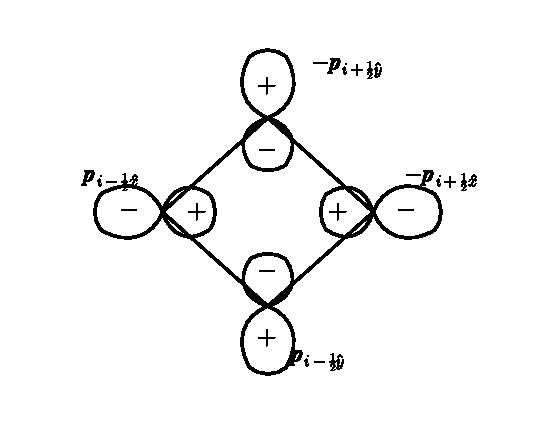
\includegraphics[width=7cm]{fig11-19.pdf}\\{\small 图 11.19\quad 氧空穴的对称组合轨道 $\boldsymbol{P}_{i\sigma}$，其中每个方块内为氧空穴波函数均具有 $\mathrm{d}_{x^{2}-y^{2}}$ 对称性}
\end{minipage}
\end{center}

$\mathrm{Cu}^{2+}$和两个氧 $(2\mathrm{p}_{x}$ 和 $2\mathrm{p}_{y})$ 轨道的三带问题简化为每个元胞中一个 $\mathrm{Cu}^{2+}$ 的 $3\mathrm{d}_{x^{2}-y^{2}}$ 轨道态 $(d_{i\sigma})$ 与一个对称组合轨道态 $(P_{i\sigma})$ 的两带杂化系统.在讨论两带杂化形成张-莱斯单重态之前，还应注意到式(11.9.24)所定义的 $P_{i\sigma}$ 不是标准的费密算子，它满足下列非正交对易关系
\begin{equation}
  \bigl[P_{i\sigma},P_{j\sigma'}^{+}\bigr]_{+}=\delta_{\sigma\sigma'}\biggl(\delta_{ij}-\frac{1}{4}\delta_{\langle ij\rangle>0}\biggr)
\end{equation}
其中仅仅在 $i$ 与j为最近邻格点时，$\delta_{\langle ij\rangle>0}=1$，而在其它情形下都等于零.利用傅里叶变换首先求出在布洛赫表象中满足费密子标准对易式 $[P_{k\sigma},P_{k'\sigma'}^{+}]_{+}=\delta_{\sigma\sigma'}\delta_{kk'}$ 的正则算符
\begin{subequations}
\begin{equation}
  P_{k\sigma}=\frac{1}{\sqrt{N}}\beta_{k}\sum_{i}P_{i\sigma}\exp(-\mathrm{i}\boldsymbol{k}\cdot\boldsymbol{R}_{i})
\end{equation}
\begin{equation}
  \beta_{k}=\biggl[1-\frac{1}{2}(\cos k_{x}+\cos k_{y})\biggr]^{-\frac{1}{2}}
\end{equation}
\end{subequations}
其中 N是 $\mathrm{CuO_{2}}$ 平面上的元胞数，并取晶格常数 $\boldsymbol{a}=\boldsymbol{1}$.再将 $P_{k\sigma}$ 变换到瓦尼尔表象
\begin{subequations}
\begin{equation}
  a_{i\sigma}=\frac{1}{\sqrt{N}}\sum_{k}P_{k\sigma}\exp(\mathrm{i}\boldsymbol{k}\cdot\boldsymbol{R}_{i})
\end{equation}
其中 $\boldsymbol{a}_{i\sigma}$ 满足费密子的标准对易关系
\begin{equation}
  \bigl[a_{i\sigma},a_{j\sigma'}^{+}\bigr]_{+}=\delta_{\sigma\sigma'}\delta_{ij}
\end{equation}
\end{subequations}
上式表明 $a_{i\sigma}$ 是瓦尼尔表象中的标准费密算子，它与非正交的 $P_{i\sigma}$ 算子间的关系可利用逆变换求出为
\begin{subequations}
\begin{equation}
  P_{i\sigma}=\sum_{j}\lambda(\boldsymbol{R}_{i}-\boldsymbol{R}_{j})a_{j\sigma}
\end{equation}
\begin{equation}
  \lambda(\boldsymbol{R}_{i}-\boldsymbol{R}_{j})=\frac{1}{N}\sum_{k}\beta_{k}^{-1}
  \exp[\mathrm{i}\boldsymbol{k}\cdot(\boldsymbol{R}_{i}-\boldsymbol{R}_{j})]
\end{equation}
\end{subequations}
对于二维正方晶格所求得的系数 $\lambda(\boldsymbol{R}_{i}-\boldsymbol{R}_{j})$ 为：当 $\boldsymbol{R}_{i}=\boldsymbol{R}_{j}$ 时取 $\lambda_{0}=0.96$，而当 $\boldsymbol{R}_{j}$ 为 $\boldsymbol{R}_{i}$ 的最近邻 Cu 格点时取 $\lambda_{1}=0.14$，次近邻值 $\lambda_{2}$ 更小，可忽略不计.这时近似用 $a_{i\sigma}+\sum_{j\in(i)}a_{j\sigma}$ 代替 $H'$ 中的 $P_{i\sigma}$ 描述两带杂化系统.在不包括非成键态的子空间中，两带系统的哈密顿量可表示为
\begin{equation}
\begin{aligned}
  H=\sum_{i,\sigma}\varepsilon_{\mathrm{d}}d_{i\sigma}^{+}d_{i\sigma}
  &+U\sum_{i}n_{i\uparrow}^{d}n_{i\downarrow}^{d}
  +\sum_{i,\sigma}\varepsilon_{\mathrm{p}}a_{i\sigma}^{+}a_{i\sigma}\\
  &+2\lambda_{0}t_{0}\sum_{i,\sigma}(d_{i\sigma}^{+}a_{i\sigma}+a_{i\sigma}^{+}d_{i\sigma})
  +2\lambda_{1}t_{0}\sum_{i,\sigma}\sum_{j\in(i)}(d_{i\sigma}^{+}a_{j\sigma}+a_{j\sigma}^{+}d_{i\sigma})
\end{aligned}
\end{equation}
其中 $a_{i\sigma}$ 是描述对称组合氧轨道上多余空穴的标准费密算子，其波函数 $a_{i\sigma}$ 具有与 $\mathrm{Cu}^{2+}$ 空穴波函数相同的 $\mathrm{d}_{x^{2}-y^{2}}$ 对称性.根据量子力学，$\boldsymbol{a}_{i\sigma}$ 上的多余空穴由于与 $\mathrm{Cu}^{2+}$ 空穴的波函数重叠大，而且相位相干(即是两个波函数的相同相位叠加)，必然有利于将此多余空穴束缚在如图11.18所示的方块之中，并与 $\mathrm{Cu}^{2+}$ 的 $3\mathrm{d}_{x^{2}-y^{2}}$ 空穴形成一个局域的自旋单重态
\begin{equation}
  b_{i}^{+}=(a_{i\uparrow}^{+}d_{i\downarrow}^{+}-a_{i\downarrow}^{+}d_{i\uparrow}^{+})/\sqrt{2}
\end{equation}
称为张-莱斯单重态.尽管也可能存在 Cu 与O空穴的自旋三重态，但却不能形成局域束缚态，其能量将比局域的自旋单重态高很多，与氢分子中的情况相似.张和莱斯的微扰估计表明：由于相位相干效应，使能量最低的自旋单重态和自旋三重态之间存在较大的能量间距，它比自旋单重态在反铁磁背景中的近邻跃迁能要高得多.因此，可以忽略单重态与三重态之间的跃迁，将系统限制在只含 Cu-O 杂化单重态的子空间之中.在前面的讨论中已经指出，在强关联情况下单占据的 $\mathrm{Cu}^{2+}$ 空穴构成超交换作用的反铁磁背景，而限制在单重态子空间中的系统在强关联极限也就自然地演变为ZRS在反铁磁背景中的隧穿运动问题，这就是张和莱斯论证系统从双带演变为有效单带的物理内容.ZRS在近邻元胞 i与j之间的隧穿能可利用式(11.9.30)中的两个 Cu-O 杂化项作微扰估计.这是一个包括 $\lambda_{0}t_{0}$（同元胞)和 $\lambda_{1}t_{0}$（近邻元胞)杂化的两步 Cu-O 是跃迁过程，其二阶跃迁矩阵元大致为 $-8\lambda_{0}\lambda_{1}(t_{0}^{2}/\Delta)\approx-(t_{0}^{2}/\Delta)$，其中包括了 Cu 与O空穴之间的自旋交换(即i元胞内的 $\mathrm{Cu}^{2+}$ 空穴通过 $\lambda_{1}t_{0}$ 杂化项跃迁到 j 元胞的氧轨道上，与此同时 i 元胞内的氧空穴因 $\lambda_{0}t_{0}$ 项作用向同元胞内的 Cu 位跃迁等过程).这样才能保证，在反铁磁背景中，跃迁后的近邻 j 元胞中也形成自旋单重态.最后，我们将说明张-莱斯的一个主要论点：在反铁磁背景中的一个局域自旋单重态(即ZRS)等效于在t-J模型中的一个空占格点态.这是因为当在i元胞内存在 ZRS 时，$\mathrm{Cu}^{2+}$ 背景中原有空穴的自旋将被O轨道上的多余空穴所屏蔽，形成总自旋为零的单态，而且是元胞(方块)范围内的局域自旋单态，将导致ZRS不再与其它元胞内的d空穴发生磁互作用.从不明显考虑氧位的观点看，可以认为一个ZRS相当于在 i 元胞内的一个等效的“安德逊 $\mathrm{Cu}^{3+}$ 态.”这时 $\mathrm{CuO_{2}}$ 层的低激发特征可以用一个类似于式(11.9.17)的推广的t-J模型描述
\begin{subequations}
\begin{equation}
\begin{aligned}
  H_{\mathrm{eff}}&=-t_{\mathrm{eff}}\sum_{\langle ij\rangle,\sigma}\bigl\{(1-n_{i\overline{\sigma}})
  C_{i\sigma}^{+}C_{j\sigma}(1-n_{j\overline{\sigma}})+h.c.\bigr\}\\
  &\quad+J_{\mathrm{eff}}\sum_{\langle ij\rangle}\biggl(\hat{\boldsymbol{S}}_{i}\cdot\hat{\boldsymbol{S}}_{j}
  -\frac{1}{4}\boldsymbol{n}_{i}\boldsymbol{n}_{j}\biggr)
\end{aligned}
\end{equation}
其中
\begin{equation}
  t_{\mathrm{eff}}=(t_{0}^{2}/\Delta),\ J_{\mathrm{eff}}=(4t_{\mathrm{eff}}^{2}/\Delta),\ \Delta=\varepsilon_{\mathrm{p}}-\varepsilon_{\mathrm{d}}
\end{equation}
\end{subequations}
为了与前文中t-J模型的符号一致.在上式中已用 $C_{j\sigma}$ 与 $C_{i\sigma}^{+}$ 代替 $d_{j\sigma}$ 与 $d_{i\sigma}^{+}$.从以上介绍可知，张-莱斯的工作主要是物理推论，而不是严格的数学证明.如何从三带赫伯德模型出发，经严格的正则变换，直接导出强关联极限下的等效t-J模型，至今尚无定论.但是ZRS概念已经为多数研究者所接受，并且在掺杂 La-214 中的 X射线吸收谱测量\textsuperscript{[32]}也支持他们关于存在 Cu-O 杂化的单重态和三重态的物理推论.张和莱斯在1988年完成的这篇短文，由于物理内涵丰富，受到超导理论研究者的普遍关注，并具有很高的引用率.

\section{高温超导体的平均场理论}

本节将从推广的t-J模型出发，在平均场近似下讨论高温超导体的d波配对和正常态能隙特征.为简单起见，将式(11.9.32)中的 $t_{\mathrm{eff}}$ 与 $J_{\mathrm{eff}}$ 仍用t 与 J表示
\begin{equation}
  H=T_{\mathrm{h}}+H_{\mathrm{J}}=-t\sum_{\langle ij\rangle,\sigma}(\hat{C}_{i\sigma}^{+}\hat{C}_{j\sigma}+h.c.)
  +J\sum_{\langle ij\rangle}\biggl(\hat{\boldsymbol{S}}_{i}\cdot\hat{\boldsymbol{S}}_{j}
  -\frac{1}{4}n_{i}n_{j}\biggr)
\end{equation}
其中 $\hat{C}_{i\sigma}$ 和 $\hat{C}_{j\sigma}^{+}$ 就是本章§7中的赫伯德投影算符[参见式(11.7.9)的附注]
\begin{subequations}
\begin{equation}
  \hat{C}_{i\sigma}^{+}=(1-n_{i\overline{\sigma}})C_{i\sigma}^{+},\quad
  \hat{C}_{j\sigma}=C_{j\sigma}(1-n_{j\overline{\sigma}})
\end{equation}
利用强关联极限下的无双占格点条件 $n_{i\uparrow}n_{i\downarrow}=0$，我们又可以用 $\hat{C}_{i\sigma}$ 与 $\hat{C}_{i\sigma}^{+}$ 代替式(11.9.18)中的 $C_{i\sigma}$ 与 $C_{i\sigma}^{+}$，将自旋1/2算符的矢量表示式写为
\begin{equation}
  \hat{\boldsymbol{S}}_{i}=\frac{1}{2}\sum_{\alpha,\beta}\hat{C}_{i\alpha}^{+}(\hat{\boldsymbol{\sigma}})_{\alpha\beta}\hat{C}_{i\beta}
\end{equation}
\end{subequations}
再利用等式
\begin{equation}
  (\hat{\boldsymbol{\sigma}})_{\alpha\beta}\bullet(\hat{\boldsymbol{\sigma}})_{\mu\nu}
  =2\delta_{\alpha\nu}\delta_{\beta\mu}-\delta_{\alpha\beta}\delta_{\mu\nu}
\end{equation}
可将反铁磁超交换作用项 $H_{\mathrm{J}}$ 改写成赫伯德投影算符的表示式
\begin{subequations}
\begin{equation}
\begin{aligned}
  H_{\mathrm{J}}&=J\sum_{\langle ij\rangle}\biggl(\hat{\boldsymbol{S}}_{i}\cdot\hat{\boldsymbol{S}}_{j}
  -\frac{1}{4}n_{i}n_{j}\biggr)\\
  &=(-J/2)\sum_{\langle ij\rangle,\sigma}
  (\hat{C}_{i\sigma}^{+}\hat{C}_{j\overline{\sigma}}^{+}\hat{C}_{j\overline{\sigma}}\hat{C}_{i\sigma}
  +\hat{C}_{i\sigma}^{+}\hat{C}_{j\overline{\sigma}}^{+}\hat{C}_{i\overline{\sigma}}\hat{C}_{j\sigma})
\end{aligned}
\end{equation}
而描述“下带”中空穴运动项的 $T_{\mathrm{h}}$ 项则直接写为
\begin{equation}
  T_{\mathrm{h}}=-t\sum_{\langle ij\rangle,\sigma}(\hat{C}_{i\sigma}^{+}\hat{C}_{j\sigma}+h.c.)
\end{equation}
\end{subequations}
这时采用隶玻色子技巧处理赫伯德投影算符 $\hat{C}_{i\sigma}$ 与 $\hat{C}_{i\sigma}^{+}$，将便于在平均场近似下进行解析研究.巴斯卡让(Baskaran)、邹(Zou)和安德逊\textsuperscript{[33]}首先建立了t-J模型的隶玻色子平均场近似理论.类似于式(11.7.13)，将投影算符 $\hat{C}_{i\sigma}^{+}(\hat{C}_{i\sigma})$ 写成标准费密算子 $f_{i\sigma}^{+}(f_{i\sigma})$ 与隶玻色子算子 $b_{i}\ (b_{i}^{+})$ 的双线性乘积：
\begin{subequations}
\begin{equation}
  \hat{C}_{i\sigma}^{+}=b_{i}f_{i\sigma}^{+},\quad \hat{C}_{i\sigma}=f_{i\sigma}b_{i}^{+}
\end{equation}
并满足类似于式(11.7.12)的强关联约束条件
\begin{equation}
  b_{i}^{+}b_{i}+\sum_{\sigma}f_{i\sigma}^{+}f_{i\sigma}=1
\end{equation}
\end{subequations}
根据他们(BZA)的观点，描述 $\mathrm{CuO_{2}}$ 平面上空占格点态的隶玻色子算子 $b_{i}$ 与 $b_{i}^{+}$ 应理解为带有电荷但无自旋的玻色子，称为空穴子，而 $f_{i\sigma}$ 与 $f_{i\sigma}^{+}$ 则描述带有1/2自旋但无电荷的费密子，又称自旋子(spinon).换句话说，是用空穴子与自旋子分别描述物理粒子的电荷与自旋自由度.

隶玻色子表示中的 $T_{\mathrm{h}}$ 与 $H_{\mathrm{J}}$ 分别为
\begin{subequations}
\begin{equation}
  T_{\mathrm{h}}=-t\sum_{\langle ij\rangle,\sigma}(b_{j}^{+}b_{i}f_{i\sigma}^{+}f_{j\sigma}+h.c.)
\end{equation}
\begin{equation}
  H_{\mathrm{J}}=-(J/2)\sum_{\langle ij\rangle,\sigma}
  \bigl(f_{i\sigma}^{+}f_{j\overline{\sigma}}^{+}f_{j\overline{\sigma}}f_{i\sigma}
  +f_{i\sigma}^{+}f_{j\overline{\sigma}}^{+}f_{i\overline{\sigma}}f_{j\sigma}\bigr)
\end{equation}
\end{subequations}
在式(11.10.6b)中本来还应有乘子 $(1+b_{i}^{+}b_{i})(1+b_{j}^{+}b_{j})$ 出现.考虑到 $\boldsymbol{\delta}=1-n$，其中 $n=\sum_{\sigma}\langle f_{i\sigma}^{+}f_{i\sigma}\rangle$，再利用约束条件的平均，有 $\langle b_{i}^{+}b_{i}\rangle=\langle b_{j}^{+}b_{j}\rangle=\delta$.当系统接近半满时，$\delta$ 只是一个小量，这时可以略去 $\boldsymbol{\delta}$ 将上述乘子近似为1.计入约束条件式(11.10.5b)和化学势 $\boldsymbol{\mu}$ 项，将隶玻色子表示中的总哈密顿量写为
\begin{equation}
  \mathscr{H}=T_{\mathrm{h}}+H_{\mathrm{J}}-\mu\sum_{i,\sigma}f_{i\sigma}^{+}f_{i\sigma}
  +\sum_{i}\lambda_{i}\biggl(b_{i}^{+}b_{i}+\sum_{\sigma}f_{i\sigma}^{+}f_{i\sigma}-1\biggr)
\end{equation}
在上式中的 $H_{\mathrm{J}}$ 还可以改写成另一种表示式
\begin{subequations}
\begin{equation}
  H_{\mathrm{J}}=-J\sum_{\langle ij\rangle}b_{ij}^{+}b_{ij}
\end{equation}
其中
\begin{equation}
  b_{ij}^{+}\equiv(f_{i\uparrow}^{+}f_{j\downarrow}^{+}-f_{i\downarrow}^{+}f_{j\uparrow}^{+})/\sqrt{2},\quad
  b_{ij}\equiv(f_{j\downarrow}f_{i\uparrow}-f_{j\uparrow}f_{i\downarrow})/\sqrt{2}
\end{equation}
\end{subequations}
代表近邻格点之间自旋子的单重态配对算符，描述产生或消灭一个价键态，而 $H_{\mathrm{J}}$ 中则包括了所有可能的近邻价键的组态，所对应的状态在量子力学中应由各种价键组态的线性组合描述，被安德逊称之为共振价键状态.根据 $b_{ij}$ 的定义式可知，在价键态中近邻格点i与j上的自旋取向是不固定的，因此共振价键状态不同于反铁磁奈耳态，它是一种没有长程序的自旋液体态.在 $H_{\mathrm{J}}$ 的表示式(11.10.8a)中出现($-$ J)因子也表明形成共振价键状态在能量上是有利的.特别是当 $\mathrm{CuO_{2}}$ 平面上存在掺杂、无序和电子-声子相互作用时，均可能有利于二维正方晶格系统中出现自旋排列的组错，从而导致共振价键状态比反铁磁奈耳态的能量更低，这就是安德逊提出从共振价键状态出发研究高温超导电性机制的主要理由.

\subsection*{1. 平均场近似解和自洽方程}

在作平均场近似时，首先设拉氏乘子 $\lambda_{i}$ 与格点位置无关 $(\lambda_{i}=\lambda)$.在物理上相当于用一个平均约束条件 $\langle b_{i}^{+}b_{i}\rangle+\sum_{\sigma}\langle f_{i\sigma}^{+}f_{i\sigma}\rangle=1$ 代替严格约束条件式(11.10.5b).在对 $T_{\mathrm{h}}$ 与 $H_{\mathrm{J}}$ 项作平均场近似处理时，需定义各类序参量，其中包括描述共振价键态的平均场参量
\begin{subequations}
\begin{equation}
  \Delta_{ij}\equiv\sqrt{2}\,\langle b_{ij}\rangle=
  \begin{cases}
    \Delta_{x} & (j=i\pm\hat{x})\\
    \Delta_{y} & (j=i\pm\hat{y})
  \end{cases}
\end{equation}
其中假定了共振价键序参量与格点i无关，只与近邻格点 i、j 间的取向有关.这里仍取二维正方晶格的元胞边长为长度的单位，$\hat{\boldsymbol{x}}$ 与 $\hat{\boldsymbol{y}}$ 分别代表x与 $y$ 方向的单位矢.再定义
\begin{equation}
  p\equiv\sum_{\sigma}\langle f_{i\sigma}^{+}f_{j\sigma}\rangle=2\langle f_{i\sigma}^{+}f_{j\sigma}\rangle
\end{equation}
\begin{equation}
  q\equiv\langle b_{j}^{+}b_{i}\rangle
\end{equation}
\end{subequations}
并设它们与格点位置、近邻格点间方向以及自旋的取向均无关，由于平均场近似使 $b_{j}^{+}b_{i}f_{i\sigma}^{+}f_{j\sigma}$ 演变为 $qf_{i\sigma}^{+}f_{j\sigma}+(p/2)b_{j}^{+}b_{i}$，可以认为 $\boldsymbol{q}$ 与 $\boldsymbol{p}$ 是描述空穴子与自旋子运动之间相互影响的平均场参量.在完成平均场近似处理后，再作傅里叶变换，最后求得t-J模型的平均场哈密顿量
\begin{equation}
\begin{aligned}
  \mathscr{H}&=\sum_{k,\sigma}\epsilon_{k}f_{k\sigma}^{+}f_{k\sigma}+\sum_{k}\omega_{k}b_{k}^{+}b_{k}
  -\sum_{k}(\Delta_{k}f_{k\uparrow}^{+}f_{-k\downarrow}^{+}+h.c.)\\
  &\quad+N\biggl(4tpq+Jp^{2}+\frac{1}{2}J\Delta_{x}^{2}+\frac{1}{2}J\Delta_{y}^{2}\biggr)
\end{aligned}
\end{equation}
其中
\begin{subequations}
\begin{equation}
  \varepsilon_{k}=-(2tq+Jp)\gamma_{k}-\mu_{f}
\end{equation}
\begin{equation}
  \omega_{k}=-2tp(\gamma_{k}-\gamma_{0})-\mu_{b}
\end{equation}
\begin{equation}
  \Delta_{k}=\sqrt{2}J(\Delta_{x}\cos k_{x}+\Delta_{y}\cos k_{y})
\end{equation}
\end{subequations}
此外，$\mu_{f}=\mu+2J(1-\delta)-\lambda$，$\mu_{b}=-\lambda-2tp\gamma_{0}$ 以及 $\gamma_{k}=\cos k_{x}+\cos k_{y}$.由于哈密顿量式(11.10.10)已简化为二次型，我们可以利用 $u\sim v$ 变换
\begin{equation}
\left.\begin{aligned}
  &f_{k\uparrow}=u_{k}^{*}\alpha_{k}+v_{k}\beta_{-k}^{+},\quad
   f_{-k\downarrow}=u_{k}^{*}\beta_{k}-v_{k}\alpha_{k}^{+}\\
  &|u_{k}|^{2}+|v_{k}|^{2}=1
\end{aligned}\right\}
\end{equation}
将 $\mathscr{H}$ 严格对角化，并得到
\begin{subequations}
\begin{equation}
\begin{aligned}
  \mathscr{H}&=\sum_{k}E_{k}(\alpha_{k}^{+}\alpha_{k}+\beta_{k}^{+}\beta_{k})
  +\sum_{k}\omega_{k}b_{k}^{+}b_{k}+\sum_{k}(\varepsilon_{k}-E_{k})\\
  &\quad+N\biggl(4tp\Delta_{b}+Jp^{2}+\frac{1}{2}J\Delta_{x}^{2}+\frac{1}{2}J\Delta_{y}^{2}\biggr)
\end{aligned}
\end{equation}
\begin{equation}
  E_{k}=\sqrt{\varepsilon_{k}^{2}+\Delta_{k}^{2}}
\end{equation}
\end{subequations}
利用公式 $G(T)=-k_{\mathrm{B}}T\ln\mathrm{Tr}(\mathrm{e}^{-\beta\mathscr{H}})$，不难求出 MFA 的吉布斯自由能
\begin{equation}
\begin{aligned}
  G(T)&=N\biggl(4tp\Delta_{b}+Jp^{2}+\frac{1}{2}J\Delta_{x}^{2}+\frac{1}{2}J\Delta_{y}^{2}\biggr)
  +\sum_{k}\varepsilon_{k}-\\
  &\quad 2k_{\mathrm{B}}T\sum_{k}\ln\bigl[2\cosh(E_{k}/2k_{\mathrm{B}}T)\bigr]
  +k_{\mathrm{B}}T\sum_{k}\ln(1-\mathrm{e}^{-\omega_{k}/k_{\mathrm{B}}T})
  +k_{\mathrm{B}}T\sum_{k}\ln\bigl[2\mathrm{e}^{-\omega_{k}/k_{\mathrm{B}}T}\bigr]
\end{aligned}
\end{equation}
根据吉布斯自由能 $G(T)$ 对 $\Delta_{\alpha}\ (\alpha=x,y)$，$\boldsymbol{q}$ 和 $\boldsymbol{p}$ 的变分极值，不难求得下列自洽方程：
\begin{subequations}
\begin{equation}
  \Delta_{\alpha}=\frac{2J}{N}\sum_{k}\Delta_{k}\cos k_{\alpha}\frac{\tanh(E_{k}/2k_{\mathrm{B}}T)}{E_{k}}
  \qquad(\alpha=x,y)
\end{equation}
\begin{equation}
  q=\frac{1}{2N}\sum_{k}\frac{\gamma_{k}}{\exp(\omega_{k}/k_{\mathrm{B}}T)-1}
\end{equation}
\begin{equation}
  p=\frac{1}{2N}\sum_{k}\gamma_{k}\biggl[1-\frac{\varepsilon_{k}}{E_{k}}\tanh\biggl(\frac{E_{k}}{2k_{\mathrm{B}}T}\biggr)\biggr]
\end{equation}
化学势 $\boldsymbol{\mu}$ 以及λ可利用 $n=(N_{e}/N)=-\dfrac{1}{N}\biggl(\dfrac{\partial G}{\partial\mu}\biggr)$ 和G对λ的变分极值求出
\begin{equation}
  1-\delta=\frac{1}{N}\sum_{k}\biggl[1-\frac{\varepsilon_{k}}{E_{k}}\tanh(E_{k}/2k_{\mathrm{B}}T)\biggr]=n
\end{equation}
\begin{equation}
  \delta=\frac{1}{N}\sum_{k}\ [\exp(\omega_{k}/k_{\mathrm{B}}T)-1]^{-1}
  =\frac{1}{N}\sum_{k}\ \langle b_{k}^{+}b_{k}\rangle
\end{equation}
\end{subequations}
它们是确定 $\boldsymbol{\mu}$ 与λ的自洽方程，实际上就是有限温度时的平均约束条件 $(1/N)\sum_{k}\langle b_{k}^{+}b_{k}\rangle+n=1$，其中 $n=(1/N)\sum_{k,\sigma}\langle f_{k\sigma}^{+}f_{k\sigma}\rangle=(1/N)\sum_{i,\sigma}\langle f_{i\sigma}^{+}f_{i\sigma}\rangle$.

\subsection*{2. d波配对与正常态存在能隙特征}

现在进一步讨论自旋子单重态配对序参量 $\Delta_{\alpha}\ (\alpha=x,y)$ 的自洽方程，在这里仅讨论下列两种情形.

\subsection*{(i) 推广的 s 波情形}

当 $\Delta_{x}=\Delta_{y}=\Delta_{\mathrm{es}}$ 时，式(11.10.15a)可表示为
\begin{subequations}
\begin{equation}
  1=(J/N)\sum_{k}(\gamma_{k}^{2}/E_{k})\tanh(E_{k}/2k_{\mathrm{B}}T)
\end{equation}
其零温自洽方程满足
\begin{equation}
\left.\begin{aligned}
  &1=\frac{J}{N}\sum_{k<k_{\mathrm{F}}}\frac{\gamma_{k}^{2}}{\sqrt{\varepsilon_{k}^{2}+(\sqrt{2}J\gamma_{k}\Delta_{\mathrm{es}})^{2}}}\\
  &\gamma_{k}=\cos k_{x}+\cos k_{y}
\end{aligned}\right\}
\end{equation}
\end{subequations}

\subsection*{(ii) d 波情形}

当 $\Delta_{x}=-\Delta_{y}\equiv\Delta_{\mathrm{d}}$ 时，从式(11.10.15a)将得到
\begin{subequations}
\begin{equation}
  1=(J/N)\sum_{k}(\eta_{k}^{2}/E_{k})\tanh(E_{k}/2k_{\mathrm{B}}T)
\end{equation}
而 $T=0$ K 时的 d 波自洽方程为
\begin{equation}
\left.\begin{aligned}
  &1=\frac{J}{N}\sum_{k<k_{\mathrm{F}}}\frac{\eta_{k}^{2}}{\sqrt{\varepsilon_{k}^{2}+(\sqrt{2}J\eta_{k}\Delta_{\mathrm{d}})^{2}}}\\
  &\eta_{k}=\cos k_{x}-\cos k_{y}
\end{aligned}\right\}
\end{equation}
\end{subequations}
比较推广s波和 d波的零温自洽方程式(11.10.16b)与式(11.10.17b)，不难看出d波配对比推广的s波配对更有利.因为对于这两个方程等式右边积分的主要贡献均来自费密面，可以近似认为 $\Delta_{\mathrm{es}}$ 与 $\Delta_{\mathrm{d}}$ 分别正比于 $\gamma_{k}$ 与 $\eta_{k}$ 在费密面上的平均值，再考虑到 $\gamma_{k}$ 的零线沿 $k_{x}+k_{y}=\pm\pi$ 和 $k_{x}-k_{y}=\pm\pi$，它们正好就是二维正方晶格在半满时的费密面.因此，在近半满时的费密面必然与 $\gamma_{k}$ 的零线比较接近，导致满足方程式(11.10.16b)的 $\Delta_{\mathrm{es}}$ 值甚小.另一方面，$\boldsymbol{\eta_{k}}$ 的零线则是沿 $k_{x}=\pm k_{y}$ 方向，即使在近半满时费密面上绝大多数点上的 $\eta_{k}$ 值与其零线相去甚远，将使满足 d 波自洽方程式(11.10.17b)的 $\Delta_{\mathrm{d}}$ 值较大，并导致 $\Delta_{\mathrm{d}}\gg\Delta_{\mathrm{es}}$.这个结果说自旋子之间的d波配对比推广的s波配对更稳定.科特里亚(Kotliar)等人\textsuperscript{[34]}的计算也证实 d 波比推广的 s 波配对具有更低的自由能.在高温超导研究中d波配对的共振价键序参量
\begin{equation}
  \Delta_{k}(T)=\sqrt{2}J\Delta_{\mathrm{d}}(T)(\cos k_{x}-\cos k_{y})
\end{equation}
又称为自旋能隙(spin gap)，它的温度依赖关系由式(11.10.17a)决定.若将 $\Delta_{k}(T_{\mathrm{RVB}})=0$ 条件代入该式，可以定出自旋子形成单重态配对的特征温度 $T_{\mathrm{RVB}}$.但这还不是超导转变温度 $T_{\mathrm{c}}$，而超导参量应当由物理上的空穴算符 $\hat{C}_{i\sigma}^{+}$ 与 $\hat{C}_{j\sigma}^{+}$ 组成单重态
\begin{equation}
  \langle\hat{C}_{i\uparrow}^{+}\hat{C}_{j\downarrow}^{+}-\hat{C}_{i\downarrow}^{+}\hat{C}_{j\uparrow}^{+}\rangle
  =\langle b_{i}b_{j}\rangle\ \langle f_{i\uparrow}^{+}f_{j\downarrow}^{+}-f_{i\downarrow}^{+}f_{j\uparrow}^{+}\rangle
\end{equation}
显然，等式右边第二个因子就是自旋子配对形成共振价键态的序参量 $\Delta_{ij}$，而第一个因子则是带电空穴子的某种凝聚，只有当 $\langle b_{i}b_{j}\rangle\neq 0$ 和 $\Delta_{ij}\neq 0$ 同时成立时系统才能进入超导状态.现已得知，存在非零的共振价键序参量的条件是 $T<T_{\mathrm{RVB}}$.至于非零的 $\langle b_{i}b_{j}\rangle$ 可能来源于单个玻色子的凝聚 $\langle b_{i}\rangle\neq 0$，也可能是由于一对近邻玻色子的凝聚.科特里亚\textsuperscript{[34]}和福山（Fukuyama)\textsuperscript{[35]}等研究均采用前一个作法，将 $\langle b_{i}b_{j}\rangle\approx\langle b_{i}\rangle\langle b_{j}\rangle\neq 0$ 简单地归结为单个空穴子的玻色凝聚，并由式(11.10.15e)决定玻色凝聚的特征温度 $T_{\mathrm{B}}$.在决定 $T_{\mathrm{B}}$ 时，首先取 $\mu_{\mathrm{b}}=0$ 条件，然后将该式改写为
\begin{equation}
  \delta=\frac{N_{0}}{N}+\frac{1}{N}{\sum_{k}}'\frac{1}{\mathrm{e}^{\beta\bar{\omega}_{k}}-1}
\end{equation}
其中 $\bar{\omega}_{k}\equiv-2tp\ (\gamma_{k}-\gamma_{0})$，$\sum'$符号表示求和不包括 $\boldsymbol{k}=\boldsymbol{0}$ 态，$N_{0}$ 则代表在零动量态上的凝聚玻色子数.众所周知，对于二维系统不存在玻色凝聚.为求出非零的 $\boldsymbol{T_{\mathrm{B}}}$，人们至少应考虑相邻的 $\mathrm{CuO_{2}}$ 面间有较小的层间跃迁 $(t_{z}\ll t)$ 的三维系统，并设
\begin{equation}
  \gamma_{k}=\cos k_{x}+\cos k_{y}+r_{z}\cos k_{z}
\end{equation}
其中 $r_{z}\equiv(t_{z}/t)$ 为小量.由此定出的玻色凝聚温度 $T_{\mathrm{B}}$ 是掺杂浓度 $\delta$ 的增长函数.图11.20是福山研究组所给出的相图曲线\textsuperscript{[35]}.由于超导电性必须在自旋子配对和玻色凝聚都出现时才可能发生.因此，当 $T_{\mathrm{B}}<T_{\mathrm{RVB}}$ 时，应取 $T_{\mathrm{c}}=T_{\mathrm{B}}$.反之，当 $T_{\mathrm{RVB}}<T_{\mathrm{B}}$ 时必须取 $T_{\mathrm{c}}=T_{\mathrm{RVB}}$.这一结果定性的说明了在超导转变温度 $T_{\mathrm{c}}$ 随 $\delta$ 变化曲线中存在一个 $T_{\mathrm{c}}$ 的最高点，与实验观测一致.更为重要的是，在欠掺杂区，当 $T_{\mathrm{RVB}}>T>T_{\mathrm{B}}$ 时，系统尚未进入超导态，但自旋子之间

\begin{center}
\begin{minipage}{6.5cm}
\centering
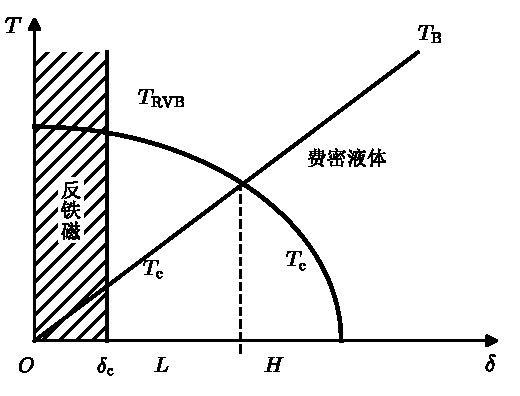
\includegraphics[width=6.5cm]{fig11-20.pdf}\\{\small 图 11.20\quad 推广 t-J模型的示意相图(其中：L——欠掺杂区，H——过掺杂区)}
\end{minipage}
\end{center}

已形成了d波配对，并存在自旋能隙，此即实验上在欠掺杂区所观测到的正常态能隙.这个具有d波对称性的能隙，在发生空穴子的玻色凝聚后，将变成超导能隙，并且有相同的 $\mathrm{d}_{x^{2}-y^{2}}$ 对称性.此外，在过掺杂区，当 $T_{\mathrm{B}}>T>T_{\mathrm{RVB}}$ 时，由于系统尚未进入共振价键状态，载流子仍然是既带电荷又有自旋的费密子，属于费密液体.福山等人还将t-J模型推广为可计入第二近邻跃迁 $t'$ 和第三近邻跃迁 $t''$ 的一个实用模型，用于计算掺杂La-214 与Y-123 等不同结构的高温超导体特性，包括计算这些化合物的非弹性中子衍射和核磁共振特性等，并且也取得了与实验测量定性一致的良好结果.有兴趣的读者可查阅文献\textsuperscript{[35]}中所列出的相关文献.

尽管基于安德逊共振价键态的超导理论能够说明大多数高温超导态与正常态特征，但是共振价键理论的基本假定(电荷与自旋分离)在两维情况下尚无严格的理论支持.仅仅在一维强关联系统中，根据赫伯德模型的严格解，理论研究已证明\textsuperscript{[36]}，低能激发可以用自旋与电荷分离的形式描写，此即一维拉亭格液体的特征.正因如此，当前强关联电子系统的一个理论研究热点是发展二维拉亭格液体理论.

在本节结束时，我们还将指出：在理论表述中描述角动量具有d波对称性时常采用 $(\cos k_{x}-\cos k_{y})$，而在实验研究中则习惯于用 $(\hat{k}_{x}^{2}-\hat{k}_{y}^{2})=\cos 2\phi$，其中 $\phi=\arctan(\hat{k}_{y}/\hat{k}_{x})$，$\hat{k}_{x}$ 与 $\hat{k}_{y}$ 是k空间单位矢 $\hat{\boldsymbol{k}}\ (|\hat{\boldsymbol{k}}|=1)$ 沿 x 与 y 方向的分量.其实只需对 $\cos k_{\alpha}\ (\alpha=x,y)$ 作形式上的级数展开，立刻可以看出 $(\cos k_{x}-\cos k_{y})$ 展开式的每一项均含有共同因子 $(k_{x}^{2}-k_{y}^{2})$，它是随k取向的快变函数，剩下的只是取向的缓变函数.再将k归一化为 $\hat{\boldsymbol{k}}$，可得到 $(\cos k_{x}-\cos k_{y})$ 正比于 $(\hat{k}_{x}^{2}-\hat{k}_{y}^{2})=\cos 2\phi$.换句话说，超导态的能隙和正常态的能隙都具有 $\mathrm{d}_{x^{2}-y^{2}}$ 对称性，与实验观测结果一致.

\section{巡游电子的磁性理论}

在第三章中我们已经证明，对于绝缘磁性材料产生磁性的局域电子在各原子周围形成局域自旋矩，它们之间的交换作用由海森伯模型描述.但是，在过渡金属中产生磁性的d电子不是局域电子，它们依次在各原子的 d轨道上游移，布洛赫称之为巡游电子(itinerant electron)，实际上就是公有化的能带电子.显然，对于巡游电子海森伯模型不成立，人们必须考虑能带电子的关联效应，从赫伯德模型入手建立巡游电子的磁性理论.根据式(11.1.13)，有外磁场 h 时的赫伯德哈密顿量为
\begin{equation}
\begin{aligned}
  &H=\sum_{k,\sigma}E_{k\sigma}n_{k\sigma}+U\sum_{l}n_{l\uparrow}n_{l\downarrow}\\
  &E_{k\sigma}=E_{k}+\sigma\mu_{\mathrm{B}}h\\
  &n_{k\sigma}=C_{k\sigma}^{+}C_{k\sigma},\quad n_{l\sigma}=C_{l\sigma}^{+}C_{l\sigma}
\end{aligned}
\end{equation}
我们将证明赫伯德哈密顿量的平均场近似(或哈特利-福克近似)就是斯通纳(Stoner)的能带磁性模型.若作无规相近似，则求得金属中的自旋波激发.

\subsection*{1. 斯通纳理论}

对H中的库仑项作哈特利-福克近似
\begin{equation}
  n_{l\uparrow}n_{l\downarrow}\approx\langle n_{l\uparrow}\rangle n_{l\downarrow}
  +\langle n_{l\downarrow}\rangle n_{l\uparrow}-\langle n_{l\uparrow}\rangle\langle n_{l\downarrow}\rangle
\end{equation}
略去等式右边的常数项并代入(11.11.1)，求得哈特利-福克近似的赫伯德哈密顿量
\begin{equation}
  H\approx\sum_{k,\sigma}E_{k\sigma}C_{k\sigma}^{+}C_{k\sigma}
  +U\sum_{l,\sigma}\langle n_{l\overline{\sigma}}\rangle C_{l\sigma}^{+}C_{l\sigma}
\end{equation}
在均匀情况下 $\langle n_{l\overline{\sigma}}\rangle$ 应与格点位置无关，这时可设
\begin{equation}
  \langle n_{\overline{\sigma}}\rangle=\langle n_{l\overline{\sigma}}\rangle
\end{equation}
再利用表象变换关系
\begin{equation}
  \sum_{l}C_{l\sigma}^{+}C_{l\sigma}=\sum_{k}C_{k\sigma}^{+}C_{k\sigma}
\end{equation}
将式(11.11.3)写成对角形式
\begin{equation}
  H\approx\sum_{k,\sigma}\widetilde{E}_{k\sigma}C_{k\sigma}^{+}C_{k\sigma}
\end{equation}
其中
\begin{equation}
  \widetilde{E}_{k\sigma}=E_{k\sigma}+U\langle n_{\overline{\sigma}}\rangle
  =E_{k}+\sigma\mu_{\mathrm{B}}h+U\langle n_{\overline{\sigma}}\rangle
\end{equation}
代表巡游电子的能量.即使在外磁场 $h=0$ 时，由于 $U\langle n_{\overline{\sigma}}\rangle$ 项的存在，$\widetilde{E}_{k\sigma}$ 仍与自旋取向有关.这时能带按自旋取向分裂，导致能带分裂的原因是由于反平行自旋电子之间的库仑排斥作用.不难证明，$U\langle n_{\overline{\sigma}}\rangle$ 项将给出一个与磁化强度M成正比的分子场.

\subsection*{(i) 分子场}

令
\begin{equation}
\left.\begin{aligned}
  &n=\langle n_{\uparrow}\rangle+\langle n_{\downarrow}\rangle\\
  &m=\langle n_{\downarrow}\rangle-\langle n_{\uparrow}\rangle
\end{aligned}\right\}
\end{equation}
其中n为平均每个元胞中的巡游电子数，$\boldsymbol{m}$ 代表相对磁化.当元胞数为N、样品取单位体积时，磁化强度
\begin{equation}
  \boldsymbol{M}=N\boldsymbol{\mu}_{\mathrm{B}}\boldsymbol{m}
\end{equation}
利用式(11.11.8)，求得
\begin{equation}
  \langle n_{\sigma}\rangle=\frac{1}{2}(n-\sigma m)=\frac{1}{2}\biggl(n-\sigma\frac{M}{N\mu_{\mathrm{B}}}\biggr)
  \qquad(\sigma=\pm 1)
\end{equation}
因此，式(11.11.7)写为
\begin{equation}
  \widetilde{E}_{k\sigma}=\biggl(E_{k}+\frac{1}{2}nU\biggr)
  +\sigma\mu_{\mathrm{B}}\biggl(h+\frac{U}{2N\mu_{\mathrm{B}}^{2}}M\biggr)
\end{equation}
上式表明，对赫伯德模型作HF近似可求出一个与M成正比的分子场
\begin{equation}
  h_{M}=\frac{U}{2N\mu_{\mathrm{B}}^{2}}M
\end{equation}
这就是斯通纳能带模型的出发点.当 $\boldsymbol{h}=\boldsymbol{0}$ 时若求得 $\langle n_{\uparrow}\rangle\neq\langle n_{\downarrow}\rangle$，则系统具有自发磁化，代表铁磁相.这时巡游电子在同一格点上的库仑作用使能带按自旋取向分裂，产生自旋朝上与向下电子数的不平衡，从而形成铁磁相，如图11.21所示，其↑、↓自旋的能带劈裂为
\begin{equation*}
  (\widetilde{E}_{k\uparrow}-\widetilde{E}_{k\downarrow})
  =U(\langle n_{\downarrow}\rangle-\langle n_{\uparrow}\rangle)\equiv 2\Delta
\end{equation*}
这里 $\langle n_{\sigma}\rangle$ 应自洽决定，而 $\Delta=\mu_{\mathrm{B}}h_{M}$.

\begin{center}
\begin{minipage}{6cm}
\centering
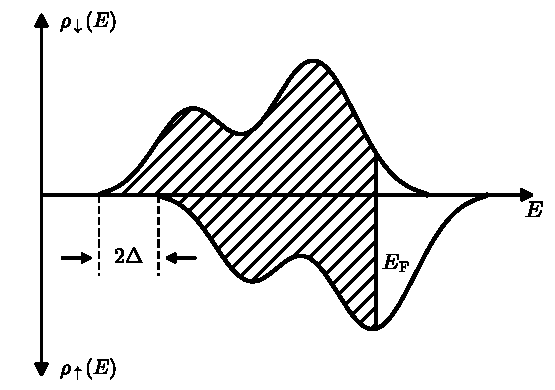
\includegraphics[width=6cm]{fig11-21.pdf}\\{\small 图 11.21\quad 过渡金属的 FM 相示意图\\
$\rho_{\uparrow}(E)$ 为自旋朝上的能带态密度，$\rho_{\downarrow}(E)$ 为自旋同下的能带态密度}
\end{minipage}
\end{center}

由于在哈特利-福克近似下哈密顿量已写成独立电子系统的标准对角化形式，根据式(11.11.6)，巡游电子在布洛赫态 $(\boldsymbol{k},\boldsymbol{\sigma})$ 上的占据数为
\begin{equation}
  \langle n_{k\sigma}\rangle=\langle C_{k\sigma}^{+}C_{k\sigma}\rangle=f(\widetilde{E}_{k\sigma})
\end{equation}
其中f是费密分布函数，适当选取能量的原点可消去式(11.11.11)中常数项 $\frac{1}{2}nU$，将 $\widetilde{E}_{k\sigma}$ 写成
\begin{equation}
\begin{aligned}
  \widetilde{E}_{k\sigma}&=E_{k}+\sigma\mu_{\mathrm{B}}\biggl(h+\frac{U}{2N\mu_{\mathrm{B}}^{2}}M\biggr)\\
  &=E_{k}+\sigma\mu_{\mathrm{B}}h+\sigma\Delta
\end{aligned}
\end{equation}
利用平移对称性，从式(11.11.4)可得
\begin{equation}
\begin{aligned}
  \langle n_{\sigma}\rangle&=\langle n_{l\sigma}\rangle=\frac{1}{N}\sum_{l}\langle n_{l\sigma}\rangle
  =\frac{1}{N}\sum_{k}\langle n_{k\sigma}\rangle\\
  &=\frac{1}{N}\sum_{k}f(\widetilde{E}_{k\sigma})
\end{aligned}
\end{equation}
代入式(11.11.9)，求得磁化强度为
\begin{equation}
\begin{aligned}
  M(T)&=N\mu_{\mathrm{B}}(\langle n_{\downarrow}\rangle-\langle n_{\uparrow}\rangle)\\
  &=\mu_{\mathrm{B}}\sum_{k}\{f(\widetilde{E}_{k\downarrow})-f(\widetilde{E}_{k\uparrow})\}
\end{aligned}
\end{equation}
当 $\boldsymbol{h}=\boldsymbol{0}$ 时，由上式可确定自发磁化与温度的关系.当 $h\neq 0$ 时，由此可以导出巡游电子系统形成铁磁相的条件.

\subsection*{(ii) 斯通纳判据}

讨论巡游电子系统中顺磁(PM)相的失稳条件，可以确定形成铁磁相的判据.设 $h=0$ 时系统处于顺磁相，有 $\langle n_{\uparrow}\rangle=\langle n_{\downarrow}\rangle$ 解.由于 $M\sim h$，当弱磁场 h作用时可以在式(11.11.16)中将 $f(\widetilde{E}_{k\sigma})$ 按h展开，求得
\begin{equation}
  M(T)\approx\mu_{\mathrm{B}}\biggl(2\mu_{\mathrm{B}}h+\frac{U}{N\mu_{\mathrm{B}}}M\biggr)
  \int_{0}^{\infty}\biggl[-\frac{\partial f(E)}{\partial E}\biggr]\rho(E)\mathrm{d}E
\end{equation}
其中 $\rho(E)$ 为能带的态密度.对于自由电子气体，取 $U=0$，得到
\begin{equation*}
  M(T)=\chi_{\mathrm{P}}(T)h
\end{equation*}
其中
\begin{equation}
  \chi_{\mathrm{P}}(T)=2\mu_{\mathrm{B}}^{2}\int_{0}^{\infty}
  \biggl(-\frac{\partial f}{\partial E}\biggr)\rho(E)\mathrm{d}E
\end{equation}
代表自由电子气体的泡利磁化率.当 $U\neq 0$ 时，对于巡游电子
\begin{equation}
  M(T)=\frac{\chi_{\mathrm{p}}(T)}{1-2\frac{U}{N}[\chi_{\mathrm{p}}(T)/4\mu_{\mathrm{B}}^{2}]}h
  \equiv\chi_{0}(T)h
\end{equation}
由此得到顺磁相的静态磁化率为
\begin{equation}
  \chi_{0}^{-1}(T)=\chi_{\mathrm{p}}^{-1}(T)-2\frac{U}{N}
\end{equation}
这里取 $4\mu_{\mathrm{B}}^{2}$ 为磁化率的单位.

当 $\chi_{0}^{-1}(T)<0$ 时顺磁相失稳，形成铁磁相.因此，根据式(11.11.20)，铁磁磁序的稳定条件为
\begin{equation}
  2\biggl(\frac{U}{N}\biggr)\chi_{\mathrm{p}}(T)>1
\end{equation}
当 $T=0$ K 时，由于 $-\dfrac{\partial f}{\partial E}=\delta(E-E_{\mathrm{F}})$，因此以 $4\mu_{\mathrm{B}}^{2}$ 为单位的泡利磁化率：
\begin{equation*}
\begin{aligned}
  \chi_{\mathrm{p}}(T=0)&=\frac{1}{2}\int\delta(E-E_{\mathrm{F}})\rho(E)\mathrm{d}E\\
  &=\frac{1}{2}\rho(E_{\mathrm{F}})
\end{aligned}
\end{equation*}
由式(11.11.21)，求得零温度时形成铁磁序的条件为
\begin{equation}
  (U/N)\rho(E_{\mathrm{F}})>1
\end{equation}
这就是铁磁相的斯通纳判据，铁磁相与顺磁相转变的相界由条件
\begin{equation}
  \chi_{0}^{-1}=0
\end{equation}
决定.例如从 $\chi_{0}^{-1}(T_{\mathrm{C}})=0$，可确定转变的居里温度 $T_{\mathrm{C}}$.

\subsection*{(iii) $T>T_{\mathrm{C}}$ 的磁化率}

对于铁磁金属，当 $T>T_{\mathrm{C}}$ 时实验上观察到磁化率满足居里-外斯（Curie-Weiss)定律
\begin{equation}
  \chi_{0}(T)=\frac{C}{T-T_{\mathrm{C}}}
\end{equation}
我们将证明斯通纳的巡游电子理论不能解释这个简单规律.根据式(11.11.20)，温度T时以 $4\mu_{\mathrm{B}}^{2}$ 为单位的磁化率为
\begin{equation}
  \chi_{0}(T)=\frac{\chi_{\mathrm{p}}(T)}{1-2I\chi_{\mathrm{p}}(T)}
\end{equation}
其中
\begin{equation*}
  I\equiv\frac{U}{N}
\end{equation*}
而泡利磁化率
\begin{equation*}
  \chi_{\mathrm{p}}(T)=\frac{1}{2}\int_{0}^{\infty}\biggl(-\frac{\partial f}{\partial E}\biggr)\rho(E)\mathrm{d}E
\end{equation*}
由于金属磁体的居里温度 $T_{\mathrm{c}}\sim 10^{2}\sim 10^{3}\ \mathrm{K}$，而费密温度 $T_{\mathrm{F}}=E_{\mathrm{F}}/k_{\mathrm{B}}\sim 10^{4}\sim 10^{5}\ \mathrm{K}$，$T_{\mathrm{F}}$ 高于金属熔点.因此，即使在 $T>T_{\mathrm{C}}$ 温区仍然有 $T\ll T_{\mathrm{F}}$ 关系，这时可算出上述费密积分
\begin{equation}
  \chi_{\mathrm{p}}(T)=\frac{1}{2}\rho_{\mathrm{F}}\biggl[1-\frac{\pi^{2}}{12}\biggl(\frac{T}{T_{\mathrm{F}}}\biggr)^{2}\biggr]
\end{equation}
它只是温度的缓变函数.代入式(11.11.25)，求得 $T>T_{\mathrm{C}}$ 时顺磁相的静态磁化率
\begin{equation}
  \chi_{0}(T)=\frac{\dfrac{1}{2}\rho_{\mathrm{F}}\biggl[1-\dfrac{\pi^{2}}{12}\biggl(\dfrac{T}{T_{\mathrm{F}}}\biggr)^{2}\biggr]}
  {[1-I\rho_{\mathrm{F}}]+I\rho_{\mathrm{F}}\dfrac{\pi^{2}}{12}\biggl(\dfrac{T}{T_{\mathrm{F}}}\biggr)^{2}}
\end{equation}
其中 $\rho_{\mathrm{F}}\equiv\rho(E_{\mathrm{F}})$ 代表费密面上的态密度.顺磁与铁磁相的转变温度 $\boldsymbol{T}_{\mathrm{C}}$ 由条件
\begin{equation}
  \chi_{0}^{-1}(T_{\mathrm{c}})=0
\end{equation}
决定.从式(11.11.28)可定出
\begin{equation}
  T_{\mathrm{C}}=T_{\mathrm{F}}\sqrt{\frac{12}{\pi^{2}}\biggl(\frac{I\rho_{\mathrm{F}}-1}{I\rho_{\mathrm{F}}}\biggr)}
\end{equation}
将此结果代入式(11.11.27)，经整理后得到磁化率与温度T的定性关系
\begin{equation}
  \chi_{0}(T)\sim\frac{T_{\mathrm{F}}^{2}}{T^{2}-T_{\mathrm{C}}^{2}}
\end{equation}
显然，这个结果与居里-外斯定律不同.因此，斯通纳的巡游电子理论不能说明 $T>T_{\mathrm{C}}$ 时磁化率的居里-外斯定律.这是理论应用于有限温区所遇到的一个重要困难.

\subsection*{(iv) 自发磁化}

令 $\widetilde{E}_{k\sigma}$ 中外磁场 $\boldsymbol{h}=\boldsymbol{0}$，从式(11.11.8)可得自发磁化方程为
\begin{equation}
\begin{aligned}
  m=\frac{M(T)}{N\mu_{\mathrm{B}}}&=\frac{1}{N}\sum_{k}(\langle n_{k\downarrow}\rangle-\langle n_{k\uparrow}\rangle)\\
  &=\frac{1}{N}\sum_{k}\{f(\widetilde{E}_{k\downarrow})-f(\widetilde{E}_{k\uparrow})\}\\
  &=\frac{1}{N}\sum_{k}\biggl\{\frac{1}{\mathrm{e}^{\beta(E_{k}-\Delta-\mu)}+1}
  -\frac{1}{\mathrm{e}^{\beta(E_{k}+\Delta-\mu)}+1}\biggr\}
\end{aligned}
\end{equation}
其中 $\beta=(k_{\mathrm{B}}T)^{-1}$，$\boldsymbol{\mu}$ 为化学势，而
\begin{equation*}
  \Delta\equiv\mu_{\mathrm{B}}h_{M}=\frac{1}{2}U(\langle n_{\downarrow}\rangle-\langle n_{\uparrow}\rangle)
\end{equation*}
$\boldsymbol{2\Delta}$ 代表↑与↓自旋能带的劈裂.当材料的能带态密度为已知时，原则上从式(11.11.31)可直接求出磁化强度与温度的关系.详细的计算见文献\textsuperscript{[37]}，在这里仅作定性介绍.从式(11.11.31)可知，磁化强度由↑、↓自旋带中电子数之差决定.因此其零温饱和磁化M(0)并不要求所有电子的自旋取向一致，这是斯通纳模型不同于海森伯模型的特点.例如当 $\mu\gg\Delta$ 时，从式(11.11.31)可求出
\begin{equation}
  \frac{M(0)}{N\mu_{\mathrm{B}}}\approx 2\Delta\int\biggl(-\frac{\partial f}{\partial E}\biggr)_{T=0}\rho(E)\mathrm{d}E
  =(2\Delta)\rho(E_{\mathrm{F}})
\end{equation}
这时平均每个元胞内的有效玻尔磁子数由能带劈裂和费密面上态密度之乘积决定，它是一个任意数，未必等于1.由此可知，在金属磁体中平均每个元胞内的零温饱和磁化强度不一定是玻尔磁子的整倍数，与实验结果一致.这是能带模型的成功之处.

当 $T\neq 0$ K 时，将产生从↓自旋带向↑自旋带的热激发.于是在↑自旋带中产生电子，而在↓自旋带中留下空穴.这种改变自旋的电子-空穴对激发称为斯通纳激发.随着温度升高斯通纳激发将使↑、↓自旋带的分裂减小，并造成 $M(T)$ 随T升高而下降，利用费密积分的索末菲展开式
\begin{equation*}
  \int_{0}^{\infty}\frac{\rho(E)}{\mathrm{e}^{\beta(E-\mu\pm\Delta)}+1}\mathrm{d}E
  =\int_{0}^{\mu\mp\Delta}\rho(E)\mathrm{d}E
  +\frac{\pi^{2}}{6}(k_{\mathrm{B}}T)^{2}\biggl(\frac{\mathrm{d}\rho}{\mathrm{d}E}\biggr)_{\mu\mp\Delta}+\cdots
\end{equation*}
从式(11.11.31)可求出在低温范围内
\begin{equation}
  \Delta M\equiv M(0)-M(T)\sim T^{2}
\end{equation}
此结果与实验测量的 $\Delta M\sim T^{3/2}$ 规律不符.这是因为斯通纳理论仍是独立电子模型，其中热激发的电子和空穴是分别独立地在平均场中运动的.在斯通纳理论中只考虑了自旋的个别激发，而忽略了自旋的集体激发.根据第三章的讨论，$\Delta M\sim T^{3/2}$ 是著名的布洛赫规律，它代表色散曲线为 $\omega=Dq^{2}$ 的自旋波激发所产生的磁化强度下降规律，这是自旋的集体激发效应.人们必须超出哈特利-福克近似，计及电子-空穴对的互作用，才能求得金属中的自旋波.我们将在“2”中用无规相近似法讨论这个问题.

\subsection*{(v) 斯通纳表述}

{\emergencystretch=2em
为了便于读者阅读有关金属磁性的文献，我们将介绍斯通纳关于铁磁性的表述.\allowbreak 根据公式(11.11.16)，以 $2\mu_{\mathrm{B}}$ 为单位的磁化强度
\begin{equation}
  M=\frac{1}{2}(N_{\downarrow}-N_{\uparrow})=\frac{1}{2}Nm
\end{equation}\par}
其中 $N_{\sigma}$ 代表自旋取向为 $\boldsymbol{\sigma}$ 的电子数，N为格点数，而m仍代表相对磁化，在这里 $N_{\sigma}=\langle n_{\sigma}\rangle N$.考虑到总电子数 $N_{e}=N_{\uparrow}+N_{\downarrow}$，平均每格点的电子浓度为 $\boldsymbol{n}=(N_{\mathrm{e}}/N)$.斯通纳引入下列量纲为1的磁序参量：
\begin{equation}
  \zeta\equiv(N_{\downarrow}-N_{\uparrow})/N_{\mathrm{e}}\qquad(0\leqslant\zeta\leqslant 1)
\end{equation}
对于铁磁相 $(\zeta\neq 0)$ 有关系式
\begin{equation}
  N_{\downarrow}=\frac{1}{2}N_{\mathrm{e}}(1+\zeta),\quad
  N_{\uparrow}=\frac{1}{2}N_{\mathrm{e}}(1-\zeta)
\end{equation}
说明↑与↓自旋的电子在k空间所占的相体积不同.对于球形等能面有 $k_{\sigma}^{\mathrm{max}}=(6\pi^{2}N_{\sigma})^{1/3}$，若再取顺磁相 $(\zeta=0)$ 的 $k_{\mathrm{F}}=(3\pi^{2}N_{e})^{1/3}$ 为波数的单位，构成的量纲为1的波数为 $k_{\sigma}\equiv(k_{\sigma}^{\mathrm{max}}/k_{\mathrm{F}})=(2N_{\sigma}/N_{\mathrm{e}})^{1/3}$，由此求得↑，↓电子的费密球半径为
\begin{equation}
  k_{\downarrow}=(1+\zeta)^{1/3},\quad k_{\uparrow}=(1-\zeta)^{1/3}
\end{equation}
当存在铁磁序 $(\zeta>0)$ 时，量纲为1的半径 $k_{\downarrow}>k_{\uparrow}$，如图11.22所示.

\begin{center}
\begin{minipage}{5.5cm}
\centering
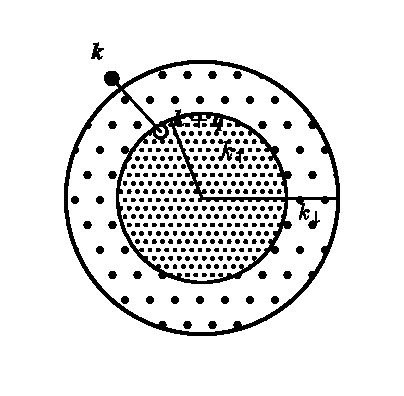
\includegraphics[width=5.5cm]{fig11-22.pdf}\\{\small 图 11.22\quad 铁磁相中↑、↓电子的费密球}
\end{minipage}
\end{center}

在无外磁场时，自旋↓与↑电子间的能带劈裂
\begin{equation}
\begin{aligned}
  2\Delta&=U(\langle n_{\downarrow}\rangle-\langle n_{\uparrow}\rangle)\\
  &=U(N_{\downarrow}-N_{\uparrow})/N\\
  &=Un\zeta
\end{aligned}
\end{equation}
利用式(11.11.14)并在球形等能面情况下取 $E_{k}=(k^{2}/2m_{\mathrm{e}}^{*})$，可将 $N_{\sigma}$ 表示为
\begin{equation*}
  N_{\sigma}=\sum_{k}f(E_{k\sigma})=\int_{0}^{\infty}\mathrm{d}E\,\rho(E)f(E+\sigma\Delta)
\end{equation*}
其中 $\rho(E)=(2m_{\mathrm{e}}^{*})^{3/2}\sqrt{E}/4\pi^{2}$，再利用索末菲展开式，即可求出 $\boldsymbol{T}=\boldsymbol{0}$ K时
\begin{equation*}
  N_{\sigma}=\frac{(2m_{\mathrm{e}}^{*})^{3/2}}{6\pi^{2}}(\mu-\sigma\Delta)^{3/2}
\end{equation*}
或更明确地写成下列表示式：
\begin{subequations}
\begin{equation}
  N_{\mathrm{e}}=\frac{N_{\mathrm{e}}}{2E_{\mathrm{F}}^{3/2}}\{(\mu+\Delta)^{3/2}+(\mu-\Delta)^{3/2}\}
\end{equation}
\begin{equation}
  2\Delta=\frac{nU}{2E_{\mathrm{F}}^{3/2}}\{(\mu+\Delta)^{3/2}-(\mu-\Delta)^{3/2}\}
\end{equation}
\end{subequations}
其中 $\boldsymbol{\mu}$ 为零温化学势，若再将 $\boldsymbol{\Delta}$ 与 $\boldsymbol{\mu}$ 均取 $E_{\mathrm{F}}$ 为能量的单位，则量纲为1的 $\boldsymbol{\mu}$ 和 $\varDelta$ 满足
\begin{subequations}
\begin{equation}
  1=\frac{1}{2}\{(\mu+\Delta)^{3/2}+(\mu-\Delta)^{3/2}\}
\end{equation}
\begin{equation}
  \zeta=\frac{1}{2}\{(\mu+\Delta)^{3/2}-(\mu-\Delta)^{3/2}\}
\end{equation}
\end{subequations}
最后求得
\begin{equation}
\begin{aligned}
  \genfrac{}{}{0pt}{}{\mu}{\Delta}\biggr\}&=\frac{1}{2}\bigl[(1+\zeta)^{2/3}\pm(1-\zeta)^{2/3}\bigr]\\
  &=\frac{1}{2}(k_{\downarrow}^{2}\pm k_{\uparrow}^{2})
\end{aligned}
\end{equation}
以上表示将对自旋波频谱的计算带来方便.若再将式(11.11.38)也写成量纲为1的表示式 $\Delta=(nU\zeta/2E_{\mathrm{F}})$，又可求得下列决定零温铁磁序参量 $\boldsymbol{\zeta}$ 的自洽方程：
\begin{equation}
\begin{aligned}
  (nU/2E_{\mathrm{F}})\zeta&=\frac{1}{2}\bigl[(1+\zeta)^{2/3}-(1-\zeta)^{2/3}\bigr]\\
  &\equiv R(\zeta)
\end{aligned}
\end{equation}
其中 $\boldsymbol{\zeta}$ 由等式左边的 $R=(nU/2E_{\mathrm{F}})\zeta$ 直线与等式右边的 $R(\zeta)$ 曲线之交点决定，如图11.23所示，由于 $R(\zeta)$ 曲线之斜率在 $\zeta=0$ 点与 $\zeta=1$ 点分别为 $(2/3)$ 与 $\infty$，可以求得3种不同的解：①顺磁解 $(\zeta=0)$：当 $(nU/2E_{\mathrm{F}})<2/3$ 时；②不完全的铁磁解 $(0<\zeta<1)$：当 $2^{-1/3}>(nU/2E_{\mathrm{F}})>2/3$ 时；③完全(饱和)铁磁解 $(\boldsymbol{\zeta}=1)$：当 $(nU/2E_{\mathrm{F}})>2^{-1/3}$ 时.换句话说，存在非零铁磁序参量 $(\zeta>0)$ 的条件为 $(nU/2E_{\mathrm{F}})>2/3$.再考虑到费密面上任一自旋取向的态密度 $\rho(E_{\mathrm{F}})=(3n/4E_{\mathrm{F}})N$，最后求得的形成铁磁序条件为
\begin{equation*}
  U(3n/4E_{\mathrm{F}})=(U/N)\rho(E_{\mathrm{F}})>1
\end{equation*}
与铁磁相的斯通纳判据式(11.11.22)一致.

\begin{center}
\begin{minipage}{5cm}
\centering
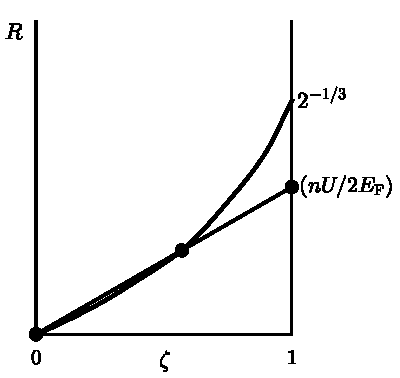
\includegraphics[width=5cm]{fig11-23.pdf}\\{\small 图 11.23\quad 确定磁序参量 $\zeta$ 的图示}
\end{minipage}
\end{center}

\subsection*{2. 金属中的自旋波}

如果超出哈特利-福克近似，用无规相近似方法讨论电子-空穴对的相互作用，可求出系统的集体激发——自旋波.在这里我们将用格林函数方法作无规相近似，其实质与第四章中讨论等离激元时所用运动方程线性化方法一致.

\subsection*{(i) 动态磁化率}

首先证明，以 $4\mu_{\mathrm{B}}^{2}$ 为单位的横向动态磁化率为
\begin{equation}
  \chi^{-+}(\boldsymbol{q},\omega)=-\langle\langle\hat{S}^{-}(\boldsymbol{q})|\hat{S}^{+}(-\boldsymbol{q})\rangle\rangle_{\omega+\mathrm{i}\eta}
\end{equation}
其中 $\hat{\boldsymbol{S}}^{\pm}(\boldsymbol{q},\omega)$ 代表自旋密度横向起伏的傅里叶分量，而格林函数 $\langle\langle\hat{S}^{-}(\boldsymbol{q})|\hat{S}^{+}(-\boldsymbol{q})\rangle\rangle_{\omega+\mathrm{i}\eta}$ 则描述金属中的自旋波.

设外磁场沿 $\nu$ 方向的分量为
\begin{equation}
  h_{\nu}(\boldsymbol{r},t)=h_{\nu}\mathrm{e}^{\mathrm{i}(\boldsymbol{q}\cdot\boldsymbol{r}-\omega t)}
\end{equation}
\begin{equation}
\begin{aligned}
  H_{\mathrm{e}}(t)&=-\sum_{\nu}\int\hat{M}_{\nu}(\boldsymbol{r})h_{\nu}\mathrm{e}^{\mathrm{i}\boldsymbol{q}\cdot\boldsymbol{r}}
  \mathrm{e}^{-\mathrm{i}(\omega+\mathrm{i}\eta)t}\mathrm{d}\boldsymbol{r}\\
  &=-\sum_{\nu}\hat{M}_{\nu}(-\boldsymbol{q})h_{\nu}\mathrm{e}^{-\mathrm{i}(\omega+\mathrm{i}\eta)t}\\
  &\equiv B\mathrm{e}^{-\mathrm{i}(\omega+\mathrm{i}\eta)t}
\end{aligned}
\end{equation}
其中 $\nu$ 方向磁化强度算符的傅里叶分量
\begin{equation}
  \hat{M}_{\nu}(\boldsymbol{q})=\int\hat{M}_{\nu}(\boldsymbol{r})\mathrm{e}^{-\mathrm{i}\boldsymbol{q}\cdot\boldsymbol{r}}\mathrm{d}\boldsymbol{r}
\end{equation}
而算符
\begin{equation}
  B=-\sum_{\nu}\hat{M}_{\nu}(-\boldsymbol{q})h_{\nu}
\end{equation}
根据久保公式
\begin{equation}
  \langle A(t)\rangle=\lim_{\eta\to+0}\mathrm{e}^{-\mathrm{i}(\omega+\mathrm{i}\eta)t}
  \langle\langle A|B\rangle\rangle_{\omega+\mathrm{i}\eta}
\end{equation}
取
\begin{equation}
  \boldsymbol{A}=\hat{\boldsymbol{M}}_{\nu}(\boldsymbol{q})
\end{equation}
可求得 $\mu$ 方向磁化强度的傅里叶分量为
\begin{equation}
\begin{aligned}
  \langle\hat{M}_{\mu}(\boldsymbol{q},\omega)\rangle&=-\sum_{\nu}
  \langle\langle\hat{M}_{\mu}(\boldsymbol{q})|\hat{M}_{\nu}(-\boldsymbol{q})\rangle\rangle_{\omega+\mathrm{i}\eta}h_{\nu}\\
  &\equiv\sum_{\nu}\chi_{\mu\nu}(\boldsymbol{q},\omega)h_{\nu}
\end{aligned}
\end{equation}
由于
\begin{equation}
  \hat{\boldsymbol{M}}=g\mu_{\mathrm{B}}\hat{\boldsymbol{S}}(\boldsymbol{r})
\end{equation}
其中 $S(\boldsymbol{r})$ 为自旋密度算符.因此，动态磁化率可以用自旋密度算符表示为
\begin{equation}
  \chi_{\mu\nu}(\boldsymbol{q},\omega)=-(g\mu_{\mathrm{B}})^{2}
  \langle\langle\hat{S}_{\mu}(\boldsymbol{q})|\hat{S}_{\nu}(-\boldsymbol{q})\rangle\rangle_{\omega+\mathrm{i}\eta}
\end{equation}
设电子的 $g=2$，并取 $4\mu_{\mathrm{B}}^{2}$ 为磁化率的单位，则求得横向动态磁化率为
\begin{equation}
  \chi^{-+}(\boldsymbol{q},\omega)=-\langle\langle\hat{S}^{-}(\boldsymbol{q})|\hat{S}^{+}(-\boldsymbol{q})\rangle\rangle_{\omega+\mathrm{i}\eta}
\end{equation}
其中 $\hat{\boldsymbol{S}}^{\pm}(\boldsymbol{q})$ 是自旋密度算符的傅里叶分量.根据附录中式(H.9)和(H.10)，$\hat{\boldsymbol{S}}^{\pm}(\boldsymbol{q})$ 可用电子算符表示成
\begin{equation}
\left.\begin{aligned}
  \hat{S}^{-}(\boldsymbol{q})&=\sum_{k}C_{k+q\downarrow}^{+}C_{k\uparrow}\\
  \hat{S}^{+}(-\boldsymbol{q})&=\sum_{k}C_{k-q\uparrow}^{+}C_{k\downarrow}
\end{aligned}\right\}
\end{equation}

\subsection*{(ii) 格林函数的无规相近似解}

从严格的赫伯德哈密顿量出发
\begin{equation*}
  H=\sum_{k,\sigma}E_{k}C_{k\sigma}^{+}C_{k\sigma}+U\sum_{l}n_{l\uparrow}n_{l\downarrow}
\end{equation*}
首先对上式作表象变换
\begin{equation*}
  C_{l\sigma}=\frac{1}{\sqrt{N}}\sum_{k}\mathrm{e}^{\mathrm{i}\boldsymbol{k}\cdot\boldsymbol{l}}C_{k\sigma}
\end{equation*}
写出布洛赫表象中的赫伯德哈密顿量
\begin{equation}
  H=H_{0}+H_{1}
\end{equation}
其中
\begin{equation}
  H_{0}=\sum_{k,\sigma}E_{k}C_{k\sigma}^{+}C_{k\sigma}
\end{equation}
\begin{equation}
  H_{1}=\frac{U}{N}\sum_{k,k',q}C_{k+q\uparrow}^{+}C_{k'-q\downarrow}^{+}C_{k'\downarrow}C_{k\uparrow}
\end{equation}
然后，利用格林函数运动方程求解.在格林函数的通式
\begin{equation}
  \omega\langle\langle A|B\rangle\rangle_{\omega}
  =\langle[A,B]\rangle-\langle\langle[H,A]|B\rangle\rangle_{\omega}
\end{equation}
中取
\begin{equation}
  B=\hat{S}^{+}(-\boldsymbol{q})=\sum_{k}C_{k-q\uparrow}^{+}C_{k\downarrow}
\end{equation}
\begin{equation}
  A=C_{k+q\downarrow}^{+}C_{k\uparrow}
\end{equation}
容易算出下列对易式
\begin{equation}
\begin{aligned}
  \langle[A,B]\rangle&=\sum_{k'}\langle[C_{k+q\downarrow}^{+}C_{k\uparrow},C_{k'-q\uparrow}^{+}C_{k'\downarrow}]\rangle\\
  &=\langle n_{k+q\downarrow}\rangle-\langle n_{k\uparrow}\rangle
\end{aligned}
\end{equation}
\begin{equation}
\begin{aligned}
  {}[H_{0},A]&=\sum_{k\sigma}E_{k}[C_{k\sigma}^{+}C_{k\sigma},C_{k+q\downarrow}^{+}C_{k\uparrow}]\\
  &=(E_{k+q}-E_{k})C_{k+q\downarrow}^{+}C_{k\uparrow}\\
  &=\omega_{kq}C_{k+q\downarrow}^{+}C_{k\uparrow}
\end{aligned}
\end{equation}
其中 $\omega_{kq}\equiv E_{k+q}-E_{k}$，库仑排斥项的对易式为
\begin{equation}
\begin{aligned}
  {}[H_{1},A]&=-\frac{U}{N}\sum_{k',q'}\bigl\{C_{k'+q'\uparrow}^{+}C_{k+q-q'\downarrow}^{+}C_{k'\uparrow}C_{k\uparrow}\\
  &\quad+C_{k+q\downarrow}^{+}C_{k'-q'\downarrow}^{+}C_{k'\downarrow}C_{k-q'\downarrow}\bigr\}
\end{aligned}
\end{equation}
由于上式右边含算符的四次项，代入格林函数方程的通式(11.11.58)将得到更高阶的格林函数.为了使格林函数方程封闭，我们将对式(11.11.63)的右边作平均场近似
\begin{equation}
\begin{aligned}
  {}[H_{1},A]&\approx U(\langle n_{\uparrow}\rangle-\langle n_{\downarrow}\rangle)C_{k+q\downarrow}^{+}C_{k\uparrow}\\
  &\quad+\frac{U}{N}(\langle n_{k+q\downarrow}\rangle-\langle n_{k\uparrow}\rangle)\sum_{k'}C_{k'+q\downarrow}^{+}C_{k'\uparrow}
\end{aligned}
\end{equation}
其中
\begin{equation*}
  \langle n_{\sigma}\rangle=\frac{1}{N}\sum_{k}\ \langle n_{k\sigma}\rangle
\end{equation*}
代入式(11.11.58)，得到线性化方程
\begin{equation}
\begin{aligned}
  &(\omega+\omega_{kq}-Um)\langle\langle C_{k+q\downarrow}^{+}C_{k\uparrow}|\hat{S}^{+}(-\boldsymbol{q})\rangle\rangle_{\omega}\\
  &=(\langle n_{k+q\downarrow}\rangle-\langle n_{k\uparrow}\rangle)
  \biggl\{1-\frac{U}{N}\sum_{k'}\langle\langle C_{k'+q\downarrow}^{+}C_{k'\uparrow}|\hat{S}^{+}(-\boldsymbol{q})\rangle\rangle_{\omega}\biggr\}\\
  &=(\langle n_{k+q\downarrow}\rangle-\langle n_{k\uparrow}\rangle)
  \biggl\{1-\frac{U}{N}\langle\langle\hat{S}^{-}(\boldsymbol{q})|\hat{S}^{+}(-\boldsymbol{q})\rangle\rangle_{\omega}\biggr\}
\end{aligned}
\end{equation}
其中
\begin{equation*}
  m=\langle n_{\downarrow}\rangle-\langle n_{\uparrow}\rangle
\end{equation*}
由此求得近似解
\begin{equation}
\begin{aligned}
  &\langle\langle C_{k+q\downarrow}^{+}C_{k\uparrow}|\hat{S}^{+}(-\boldsymbol{q})\rangle\rangle_{\omega}
  =\frac{f(E_{k+q\downarrow})-f(E_{k\uparrow})}{\omega+\omega_{kq}-Um}\times\\
  &\quad\biggl\{1-\frac{U}{N}\langle\langle\hat{S}^{-}(\boldsymbol{q})|\hat{S}^{+}(-\boldsymbol{q})\rangle\rangle_{\omega}\biggr\}
\end{aligned}
\end{equation}
这里取哈特利-福克近似的
\begin{equation}
\begin{aligned}
  &\langle n_{k\sigma}\rangle=f(E_{k\sigma})\\
  &E_{k\sigma}=E_{k}+U\langle n_{\overline{\sigma}}\rangle
\end{aligned}
\end{equation}
$\boldsymbol{f}$ 为费密分布函数，这种运动方程的线性化近似就是无规相近似，有时也称为动态平均场近似.根据式(11.11.54)，将式(11.11.66)对 k 求和后得到 $\langle\langle\hat{S}^{-}(\boldsymbol{q})|\hat{S}^{+}(-\boldsymbol{q})\rangle\rangle_{\omega}$.因此，铁磁相的无规相近似动态磁化率为
\begin{equation}
  \chi^{-+}(\boldsymbol{q},\omega)=-\langle\langle\hat{S}^{-}(\boldsymbol{q})|\hat{S}^{+}(-\boldsymbol{q})\rangle\rangle_{\omega+\mathrm{i}\eta}
  =\frac{\Gamma^{-+}(\boldsymbol{q},\omega)}{1-\dfrac{U}{N}\Gamma^{-+}(\boldsymbol{q},\omega)}
\end{equation}
其中
\begin{equation}
\begin{aligned}
  \Gamma^{-+}(\boldsymbol{q},\omega)&=-\sum_{k}\frac{f(E_{k+q\downarrow})-f(E_{k\uparrow})}
  {\omega+(E_{k+q\downarrow}-E_{k\uparrow})+\mathrm{i}\eta}\\
  &=\sum_{k}\frac{f(E_{k+q\uparrow})-f(E_{k\downarrow})}
  {\omega-(E_{k+q\uparrow}-E_{k\downarrow})+\mathrm{i}\eta}
\end{aligned}
\end{equation}
在后一等式中，作了变量代换 $\boldsymbol{k}\to-\boldsymbol{k}-\boldsymbol{q}\ (-\boldsymbol{k}\to\boldsymbol{k}+\boldsymbol{q})$ 并利用了 $\boldsymbol{E}_{-\boldsymbol{k}}=\boldsymbol{E}_{\boldsymbol{k}}$ 对称性.这时 $\Gamma^{-+}(\boldsymbol{q},\omega)$ 的极点为
\begin{equation}
  E_{k+q\uparrow}-E_{k\downarrow}=\omega_{kq}+Um
  =(E_{k+q}-E_{k})+U(\langle n_{\downarrow}\rangle-\langle n_{\uparrow}\rangle)
\end{equation}
对于顺磁相，$\langle n_{\uparrow}\rangle=\langle n_{\downarrow}\rangle$，$(E_{k+q\uparrow}-E_{k\downarrow})=(E_{k+q}-E_{k})$，这时
\begin{equation}
  \mathrm{Re}\,\Gamma^{-+}(q=0,\omega=0)=\sum_{k}\biggl(-\frac{\partial f}{\partial E_{k}}\biggr)=2\chi_{\mathrm{p}}(T)
\end{equation}
在这里 $\chi_{\mathrm{p}}(T)$ 就是自由电子气的泡利顺磁磁化率.由此可知，对于顺磁相，$\Gamma^{-+}(\boldsymbol{q},\omega)$ 代表无相互作用系统的横向动态磁化率.

\subsection*{(iii) 元激发谱}

互作用系统的元激发由格林函数 $\langle\langle\hat{S}^{-}|\hat{S}^{+}\rangle\rangle_{\omega}$（或 $\chi^{-+}$）的极点决定.根据式(11.11.68)，决定这些极点的本征方程为
\begin{equation}
  F(\omega)\equiv\frac{U}{N}\sum_{k}\frac{f(E_{k+q\uparrow})-f(E_{k\downarrow})}
  {\omega-(E_{k+q\uparrow}-E_{k\downarrow})}=1
\end{equation}
与等离激元问题相似，在 $\boldsymbol{T}=\boldsymbol{0}$ K 时作 $F(\omega)$ 曲线，它与直线 $F(\omega)=1$ 之交点代表系统的元激发.如图11.24所示.其中有一组准连续的交点落在 $F(\omega)$ 的发散点附近，可近似取为
\begin{equation}
  \omega=E_{k+q\uparrow}-E_{k\downarrow}=(E_{k+q}-E_{k})+U(\langle n_{\downarrow}\rangle-\langle n_{\uparrow}\rangle)
\end{equation}
此即 $\Gamma^{-+}(\boldsymbol{q},\omega)$ 的极点，它代表↑、↓自旋带之间的电子-空穴对激发，称为斯通纳激发或个别激发.当 $T=0$ K 时由于费密球的限制，斯通纳激发有上界 $\omega_{\mathrm{max}}$ 和下界 $\omega_{\mathrm{min}}$.从式(11.11.69)不难看出，在斯通纳区 $\omega_{\mathrm{min}}<\omega<\omega_{\mathrm{max}}$ 内 $\mathrm{Im}\,\Gamma^{-+}(\boldsymbol{q},\omega)\neq 0$，而在此区域之外 $\mathrm{Im}\,\Gamma^{-+}(\boldsymbol{q},\omega)=0$.这说明↑、↓自旋带之间的电子-空穴对个别激发(斯通纳激发)是有阻尼的.此外，在图11.24的低频端还存在一个交点，由于此交点落在斯通纳区之外 $(\omega<\omega_{\mathrm{min}})$，在零温时这个解是无阻尼的，它代表互作用系统的自旋集体振荡，即金属中的自旋波的色散曲线，可以讨论方程式(11.11.72)在长波和低频范围内的近似解.首先，对式(11.11.72)作变量代换，得到

\begin{center}
\begin{minipage}{7cm}
\centering
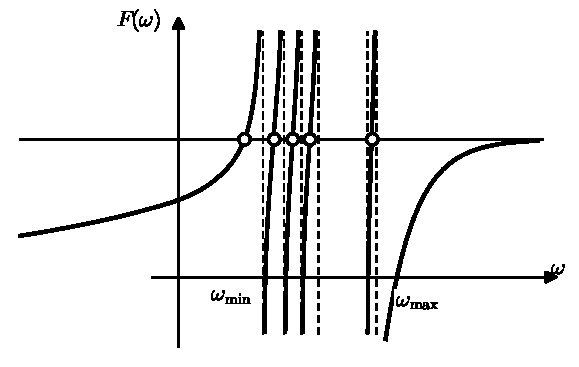
\includegraphics[width=7cm]{fig11-24.pdf}\\{\small 图 11.24\quad 方程式(11.11.72)的根}
\end{minipage}
\end{center}

\begin{equation}
  1=F(\omega)=\frac{U}{N}\sum_{k}\biggl\{\frac{f_{k\downarrow}}{mU-\omega+(E_{k+q}-E_{k})}
  -\frac{f_{k\uparrow}}{mU-\omega-(E_{k-q}-E_{k})}\biggr\}
\end{equation}
其中
\begin{equation}
  f_{k\sigma}\equiv f(E_{k\sigma})
\end{equation}
在长波范围内可作下列展开：
\begin{equation}
  E_{k\pm q}-E_{k}=\pm(\boldsymbol{q},\nabla)E_{k}+\frac{1}{2}(\boldsymbol{q}\cdot\nabla)^{2}E_{k}
\end{equation}
由于在铁磁相 $mU$ 取有限值，因此当 $q\to 0,\ \omega\to 0$ 时可取 $\omega/mU$ 和 $(E_{k\pm q}-E_{k})/mU$ 作为展开的小参量.将式(11.11.74)中分母展开到 $q^{2}$ 项，得到
\begin{equation*}
\begin{aligned}
  1=F(\omega)&=\biggl(1+\frac{\omega}{mU}\biggr)\frac{1}{mN}\sum_{k}(f_{k\downarrow}-f_{k\uparrow})
  -\frac{1}{2m^{2}UN}\sum_{k}(f_{k\uparrow}+f_{k\downarrow})(\boldsymbol{q}\cdot\nabla)^{2}E_{k}\\
  &\quad+\frac{1}{2m^{3}U^{2}N}\sum_{k}(f_{k\downarrow}-f_{k\uparrow})(\boldsymbol{q}\cdot\nabla E_{k})^{2}
\end{aligned}
\end{equation*}
考虑到
\begin{equation*}
  m=\langle n_{\downarrow}\rangle-\langle n_{\uparrow}\rangle=\frac{1}{N}\sum_{k}(f_{k\downarrow}-f_{k\uparrow})
\end{equation*}
并设 $E_{k}$ 为球形等能面.这时将有近似式
\begin{equation}
\begin{aligned}
  1=F(\omega)&=\biggl(1+\frac{\omega}{mU}\biggr)-\frac{q^{2}}{2m^{2}UN}\sum_{k}(f_{k\uparrow}+f_{k\downarrow})\nabla^{2}E_{k}\\
  &\quad+\frac{q^{2}}{3m^{2}U^{2}N}\sum_{k}(f_{k\downarrow}-f_{k\uparrow})(\nabla E_{k})^{2}
\end{aligned}
\end{equation}
由此求得自旋波的色散曲线
\begin{equation}
  \omega=Dq^{2}
\end{equation}
其中
\begin{equation}
  D=\frac{1}{2mN}\biggl\{\sum_{k}(f_{k\uparrow}+f_{k\downarrow})\nabla^{2}E_{k}
  -\frac{2}{3mU}\sum_{k}(f_{k\downarrow}-f_{k\uparrow})(\nabla E_{k})^{2}\biggr\}
\end{equation}
称为自旋波的劲度系数.我们将举例证明在球形等能面情况下 $\boldsymbol{D}>\boldsymbol{0}$.

例如 $\boldsymbol{T}=\boldsymbol{0}$ K时自旋波劲度系数D的计算.

在球形等能面情况，设 $E_{k}=(k^{2}/2m_{\mathrm{e}}^{*})$，这时 $\nabla^{2}E_{k}=(1/m_{\mathrm{e}}^{*})$，而 $(\nabla E_{k})^{2}=\nabla E_{k}\cdot\nabla E_{k}=(k/m_{\mathrm{e}}^{*})^{2}$，式(11.11.79)在取 $k_{\mathrm{F}}$ 为波数的单位时可改写为
\begin{equation*}
  D=\frac{1}{2m}\cdot\frac{k_{\mathrm{F}}^{2}}{2m_{\mathrm{e}}^{*}}\cdot\frac{1}{N}\sum_{k}(f_{k\uparrow}+f_{k\downarrow})
  -\frac{1}{3m^{2}NU}\cdot\frac{k_{\mathrm{F}}^{5}}{(m_{\mathrm{e}}^{*})^{2}}\sum_{k}(f_{k\downarrow}-f_{k\uparrow})k^{2}
\end{equation*}
其中相对磁化 $m=n\zeta$，而 $\boldsymbol{n}=(N_{\mathrm{e}}/N)$.当 $\boldsymbol{T}=\boldsymbol{0}$ K 时，考虑到
\begin{equation*}
  \frac{1}{N}\sum_{k}(f_{k\uparrow}+f_{k\downarrow})=N_{\mathrm{e}}/N=n
\end{equation*}
\begin{equation*}
\begin{aligned}
  \frac{1}{N}\sum_{k}(f_{k\downarrow}-f_{k\uparrow})k^{2}
  &=\frac{1}{2\pi^{2}}\biggl\{\int_{0}^{k_{\downarrow}}k^{4}\mathrm{d}k-\int_{0}^{k_{\uparrow}}k^{4}\mathrm{d}k\biggr\}\\
  &=\frac{1}{10\pi^{2}}(k_{\downarrow}^{5}-k_{\uparrow}^{5})
\end{aligned}
\end{equation*}
可将D写成
\begin{equation*}
  D=\frac{E_{\mathrm{F}}}{\zeta}\biggl\{1-\biggl(\frac{2E_{\mathrm{F}}}{mU}\biggr)\cdot\frac{1}{5}\cdot(k_{\downarrow}^{5}-k_{\uparrow}^{5})/\zeta\biggr\}
\end{equation*}
其中利用了 $k_{\mathrm{F}}^{3}=3\pi^{2}N_{\mathrm{e}}$ 和 $E_{\mathrm{F}}=(k_{\mathrm{F}}^{2}/2m_{\mathrm{e}}^{*})$.从式(11.11.38)可知 $\frac{1}{2}nU\zeta=\Delta$，再利用式(11.11.41)求得 $(nU\zeta/2E_{\mathrm{F}})=(k_{\downarrow}^{2}-k_{\uparrow}^{2})/2$.因此，在取 $\boldsymbol{E}_{\mathrm{F}}$ 为能量的单位时，所求出的自旋波劲度系数D为
\begin{equation*}
\begin{aligned}
  D&=\frac{1}{\zeta}\biggl\{1-\frac{2}{5}\frac{(k_{\downarrow}^{5}-k_{\uparrow}^{5})}{(k_{\downarrow}^{2}-k_{\uparrow}^{2})}\biggr\}\\
  &=\frac{1}{\zeta}\biggl\{1-\frac{2}{5}\frac{(1+\zeta)^{5/3}-(1-\zeta)^{5/3}}{(1+\zeta)^{2/3}-(1-\zeta)^{2/3}}\biggr\}>0
  \quad(0<\zeta\leqslant 1\ \text{时})
\end{aligned}
\end{equation*}
这就是 $\boldsymbol{D}>\boldsymbol{0}$ 的证明.显然，当 $\zeta\ll 1$ 时，经展开可得 $D\approx\zeta/9>0$，而当 $\boldsymbol{\zeta}\to 1$ 时(完全铁磁情形)，$D=1/5>0$.图 11.25 中绘出了自旋波的色散曲线，和斯通纳电子-空穴对激发区，其中集体激发位于个别激发区之下.显然，在低温区自旋波激发将起主要作用.利用自旋波色散关系 $\omega\sim q^{2}$，容易证明：由于激发自旋波量子所引起低温磁化的降低 $\Delta M\sim T^{3/2}$，与实验结果一致，改进了斯通纳(哈特利-福克近似)理论.

\begin{center}
\begin{minipage}{7cm}
\centering
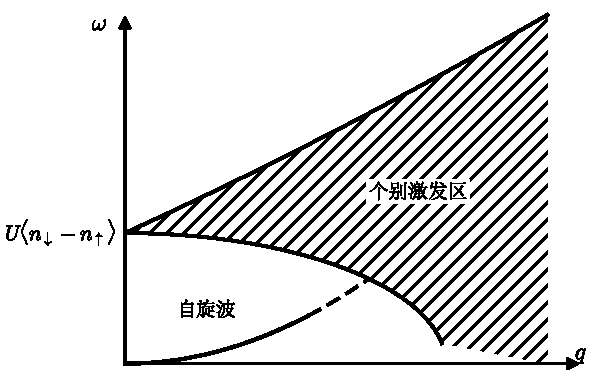
\includegraphics[width=7cm]{fig11-25.pdf}\\{\small 图 11.25\quad 铁磁金属的元激发谱}
\end{minipage}
\end{center}

\subsection*{3. HFA 和 RPA 理论的困难}

前面已经说明，从哈特利-福克近似理论不能推导出 $T>T_{\mathrm{C}}$ 时磁化率的居里-外斯定律，这是斯通纳理论应用于有限温度的主要困难.试问从无规相近似理论是否能得到居里-外斯定律？为此，我们讨论无规相近似的横向动态磁化率的长波 $(\boldsymbol{q}=0)$ 静态 $(\omega=0)$ 极限.根据式(11.11.68)—(11.11.71)，当 $T>T_{\mathrm{C}}$ 时顺磁相的长波静态磁化率为
\begin{equation}
  \chi^{-+}=\frac{\Gamma^{-+}(0,0)}{1-I\Gamma^{-+}(0,0)}
  =2\frac{\chi_{\mathrm{p}}(T)}{1-2I\chi_{\mathrm{p}}(T)}\qquad(q=0,\omega=0)
\end{equation}
其中 $I=U/N$.对于各向同性磁体，横向静态磁化率应为纵向之二倍.因此，从式(11.11.80)所求得的纵向静态顺磁磁化率
\begin{equation*}
  \chi_{0}(T)=\frac{\chi_{\mathrm{p}}(T)}{1-2I\chi_{\mathrm{p}}(T)}
\end{equation*}
它与哈特利-福克近似的磁化率公式(11.11.25)一样.在这里哈特利-福克近似和无规相近似理论碰到了相同的困难：$\chi_{0}(T)$ 的温度关系完全由泡利磁化率 $\chi_{\mathrm{p}}(T)$ 决定，而后者在 $T\ll T_{\mathrm{F}}$ 时只是温度的缓慢变化函数，它们都不能解释 $\boldsymbol{T}>\boldsymbol{T}_{\mathrm{C}}$ 时铁磁金属中所观察到的磁化率的居里-外斯定律.此外，从 $\chi_{0}^{-1}(T_{\mathrm{c}})=0$ 所求得居里温度 $T_{\mathrm{C}}$ 的理论值也比实测值高很多.

斯通纳理论在有限温度失败的原因是由于所采用的哈特利-福克近似对热激发效应估计不充分.它用↑，↓自旋带间电子与空穴的个别激发来说明金属磁的有限温度特性，认为电子和空穴是分别、独立的在平均场中运动，忽略了热激发的准粒子之间的关联作用.因此，斯通纳理论只是一种建立在单电子近似基础上的平均场理论，它所建立的热平衡图像是：$T=0$ K 时产生铁磁磁序的↑、↓自旋带分裂，将因温度升高和电子-空穴对激发加骤而逐渐减小.在 $T_{\mathrm{C}}$ 以上，就成为没有能带分裂的顺磁相，而具有泡利顺磁性.这就是斯通纳的热平衡态.从多体理论的角度，这样的描述是不完善的.实际上，在互作用系统中，热激发的电子和空穴之间的关联作用十分重要.首先，它将在铁磁金属中产生电子自旋密度的涨落，并以集体激发的形式传播，表现为各种 $\boldsymbol{q}$ 模式的自旋涨落波.当 $T<T_{\mathrm{C}}$ 时，相对于铁磁基态的自旋涨落可以近似用自旋波图像描述.其次，这些自旋涨落模还将通过模-模耦合作用对铁磁金属的热平衡态($\boldsymbol{q}=\boldsymbol{0}$模)产生重要的影响.无规相近似理论近似计算了相对于斯通纳热平衡态的自旋涨落，求得了金属中的自旋波激发等正确结果.但是，另一方面由于无规相近似略去了不同自旋模式之间的相互作用.因此，从无规相近似理论所求得的顺磁相磁化率仍然与斯通纳理论一样，也不能说明居里-外斯定律.在这个意义上人们常说无规相近似没有自洽的计入自旋涨落效应.现已明白，在铁磁金属中真正的顺磁态，不是斯通纳理论所描述的泡利顺磁性状态，它还应当包括各种可能激发的自旋涨落模，并且这些自旋涨落模式通过模-模耦合作用还将对斯通纳平衡态产生重要修正.因此，为了克服 $T>0$ K 时斯通纳理论的缺点，必须超出无规相近似范围，建立自洽计入自旋涨落效应的理论.在这方面日本物理学家守谷亨(Moriya)作出了重要贡献.他建立了弱铁磁金属自旋涨落的自洽重正化理论(self consistent renormalization theory，简称 SCR理论)\textsuperscript{[38]}，并在巡游电子模型中导出了磁化率的居里-外斯定律，其理论与弱铁磁金属如 $\mathrm{ZrZn_{2}}\,[T_{\mathrm{C}}=25\,\mathrm{K},\ M(0)/N\mu_{\mathrm{B}}=0.12]$ 和 $\mathrm{Sc_{3}In}\,[T_{\mathrm{C}}=6\,\mathrm{K},\ M(0)/N\mu_{\mathrm{B}}=0.04]$ 中的实验测量结果符合良好.SCR理论指出：在弱铁磁金属中由于长波自旋涨落压制磁化，将使 $T>T_{\mathrm{C}}$ 时静态磁化率服从居里-外斯定律，这是居里-外斯定律的新解释.

在20世纪80年代 SCR理论曾有较大的进展，并已超出弱铁磁金属范围成为巡游电子的自旋涨落理论.守谷亨曾寄希望于能够在自旋涨落理论的基础上建立金属磁性的统一图像\textsuperscript{[39]}.近年来自旋涨落的 SCR理论用于解释铜氧化合物高温超导体的正常态能隙也取得了成功\textsuperscript{[40]}.

\begin{canKao}
\begin{enumerate}[label={[\arabic*]}, leftmargin=2.2em, itemsep=0pt]
\item Hubbard J. Proc Roy Soc (London), 1963, A276: 238
\item Zubarev D N. Soviet Phys Usp (English Trasl), 1960, 3: 320
\item Hubbard J. Proc Roy Soc (London), 1964, A281: 401
\item Anderson P W. Phys Rev, 1961, 124: 41
\item Appelbaum J A. Lectures in Theoret Phys, 1971, XII-A: 41
\item Blandin A. J Appl Phys, 1967, 38: 1143
\item Leder H J, Mühlshlegel B. Z Phys, 1978, B29: 341
\item Kasuya T. Prog Theoret Phys (Kyoto), 1956, 16: 45
\item Ruberman M A, Kittle C. Phys Rev, 1954, 96: 99
\item Yosida K. Phys Rev, 1969, 106: 893
\item Nagamiya T. Solid State Physics, 1967, 20: 306
\item Darby M I. Am J Phys, 1969, 37: 354
\item Kittle C. Quantum Theory of Solids. New York: John Wiley and Sons Inc, 1963. Chap 18
\item Merzbacher E. Quantum Mechanics (2nd ed). New York: John Wiley and Sons Inc, 1970. Chap 12
\item van Vleck J H. Rev Mod Phys, 1962, 34: 681
\item Hathaway K B. Ultrathin Magnetic Structures. In: Heinrich B et al, ed. Berlin: Spinger--Verley, 1994. Chap 2
\item 李正中. 物理，1982，11：101
\item Kondo J. Solid State Physics, 1969, 23: 183
\item Yosida K. Phys Rev, 1966, 147: 223
\item Wilson K G. Rev Mod Phys, 1975, 47: 773
\item Andrei N. Phys Rev Lett, 1980, 45: 379
\item Wiegmann P B. Pis'ma Zh Eksep Teor Fiz, 1980, 31: 392
\item Schrieffer J R, Wolff P A. Phys Rev, 1966, 149: 491
\item Hewson A C. The Kondo Problem to Heavy Fermions. New York: Cambridge Univ Press, 1993
\item Degiorgi L. Rev Mod Phys, 1999, 71: 687
\item Coleman P S. Phys Rev, 1984, B29: 3035; 1987, B35: 5072
\item Read N, Newsn D M. Solid State Commun, 1984, 52: 993
\item Newsn D M, Read N. Adv Phys, 1987, 36: 799
\item Balacandran A P et al. Int J Mod Phys, 1990, 4: 2057
\item Zaanen J et al. Phys Rev, 1988, B37: 9423
\item Zhang F C, Rice T M. Phys Rev, 1988, B37: 3759; 1990, 41: 7243
\item Romberg H et al. Phys Rev, 1990, B42: 8768
\item Baskaram G, Zou Z, Anderson P W. Solid State Commun, 1987, 63: 973
\item Kotliar G, Liu J. Phys Rev, 1988, B38; 5142
\item Fukuyama H et al. Physica, 1997, 282--287: 124
\item Lieb E H, Wu F Y. Phys Rev Lett, 1968, 20: 1445
\item Wohlfarth E P. Rev Mod Phys, 1953, 25: 211
\item Moriya T. JMMM, 1979, 14: 1
\item Moriya T. Spin Fluctuations in Itinerant Electron Magmetisin. Berlin: Springer--Verlag, 1985
\item Imada M et al. Rev Mod Phys, 1998, 70: 1039
\end{enumerate}
\end{canKao}